\chapter{Quasar Emission Lines as Probes of Orientation and Unification}



{\em This chapter is based on a paper in preparation:

Matthews J. H., Knigge C., 
`Quasar Emission Lines as Probes of Orientation and Unification',
to be submitted to MNRAS.}


%%%%%%%%%%%%%%%%%%%%%%%%%%%%%%%%%%%%%%
%
%          ABSTRACT
%
%%%%%%%%%%%%%%%%%%%%%%%%%%%%%%%%%%%%%%%
\maketitle

\section{Introduction}

In the previous chapter, I presented tests of geometric unification
models using MCRT and photoionization simulations. 
One of the key results from that analysis is that trends with
inclination prohibit models with equatorial outflows matching
observations, as the EWs of the broad emission lines tend
to increase with inclination. This conclusion is strongly dependent 
on the outflow geometry and suggests that understanding the orientations
of BALQSOs, or, equivalently, the opening angles of their winds, is crucially
important if we are to establish the validity of geometric unification
models. The motivation to measure orientations is not limited to disc wind models; the
AM85 and UP95 unification schemes described in section~\ref{agn_unification}
both attempt to explain the diverse behaviour of AGN merely as a function of viewing 
angle. Orientation indicators therefore also allow us to explore if these models
adequately explain the type 1/type 2 dichotomy in AGN.
Furthermore, constraining outflow geometries is not only important 
for unification. The covering factor and opening angle of the outflow
are important quantities for estimating the
feedback efficiency \citep[e.g.][]{borguet2012}, measuring
the BAL fraction \citep[e.g.][]{krolikvoit1998}
and understanding the outflow physics \citep[e.g.][]{proga2005}. 

Unlike in galactic accretion disc systems, measuring inclinations
for quasars and AGN is notoriously difficult. Obtaining 
reliable orientation indicators is thus an important observational
goal for the community \citep[see e.g.][]{marin2016}. 
Perhaps as a result of this problem, 
directly opposing geometries have been proposed for 
BAL outflows (see section~\ref{sec:balqsos}). 
Attempts to constrain the inclinations
of BALQSOs have been made previously with
different diagnostics; for example, by considering 
radio measurements \citep{zhou2006,dipompeo2012a}, 
polarisation \citep{brotherton2006}
and emission line properties \citep{dipompeo2012b}.  

One potential way to estimate quasar inclination is by comparing
the emergent flux of a roughly isotropic emission line to the continuum, which is
expected to be strongly anisotropic if it is emitted from a geometrically thin, 
optically thick accretion disc. 
It follows that, if we can estimate the angular distribution of line and continuum emission,
the EW of an emission line can act as an orientation indicator. Conversely, if the orientations
of quasars were well-known then the emission line EW distribution could be used to test models
for the origin of the UV and optical continuum.
The variation of EW with inclination is demonstrated neatly by the behaviour 
of emission lines in high-state CVs, where inclinations are fairly well constrained.
High-state CVs show a clear trend of increasing line EW with inclination 
\citep[][see also sections~\ref{sec:NLs} and \ref{sec:modela_spectra}]{hessman1984,patterson1984,echevarria1988,noebauer},
a trend that is attributed to foreshortening and lib darkening of the disc continuum.

The ideal emission line to use for this method would be one that is completely isotropic,
i.e. {\em optically thin}. The \oiiifull\ narrow emission line is a strong, forbidden line
formed in the narrow-line region (NLR) of AGN, and should thus be completely isotropic.
Any dispersion in the distribution of \oiiifull\ EW (\ewo) must therefore be driven by some combination of
the intrinsic luminosity \citep{borosongreen} 
the covering factor/geometry of the NLR \citep{baskin2005} and the 
inclination of the disc. In a recent study, \citet{risaliti2011} showed that 
the \ewo\ distribution could be well-fitted by a simple model driven purely by disc inclination.
In this chapter, I apply a similar method in order to provide a fundamental test of
BAL and non-BAL quasar unification models in which the continuum source is a geomtrically
thin, optically thick disc. This is motivated by the remarkably similar
emission line properties of BAL and non-BAL quasars -- a similarity that would not
be expected from the simplest models in which BALQSOs are viewed from equatorial angles.

This chapter is structured as follows. First, I describe
the data sample and selection criteria being used. I begin by
simply examining the distributions of the EW of the \oiiifull\ emission line,
\ewo, and comparing the BAL and non-BAL quasar distributions. 
In section~\ref{sec:disc_agn}, I review the angular distribution of 
continuum emission one would expect from simple $\alpha$-disc models, 
as well as exploring more advanced disc models computed
with \agn. I then use these theoretical 
angular distributions applied to a simple toy model in 
section~\ref{sec:mc_angular}, and conduct MC simulations in an attempt to fit 
the observed LoBAL and non-BAL quasar distributions of \ewo, using a similar approach to 
\cite{risaliti2011}. In section~\ref{sec:discuss_ew}, I discuss the results
in the context of radio and polarisation measurements of AGN,
and explore the location of BAL quasars in `Eigenvector 1' parameter space.
I also consider the broad emission line distribution in HiBAL quasars in more detail. 
Finally, in section~\ref{sec:ew_conclusions}, I summarise the results.


\section{Data Sample}

% \begin{figure*} %fullpage
% \centering
% 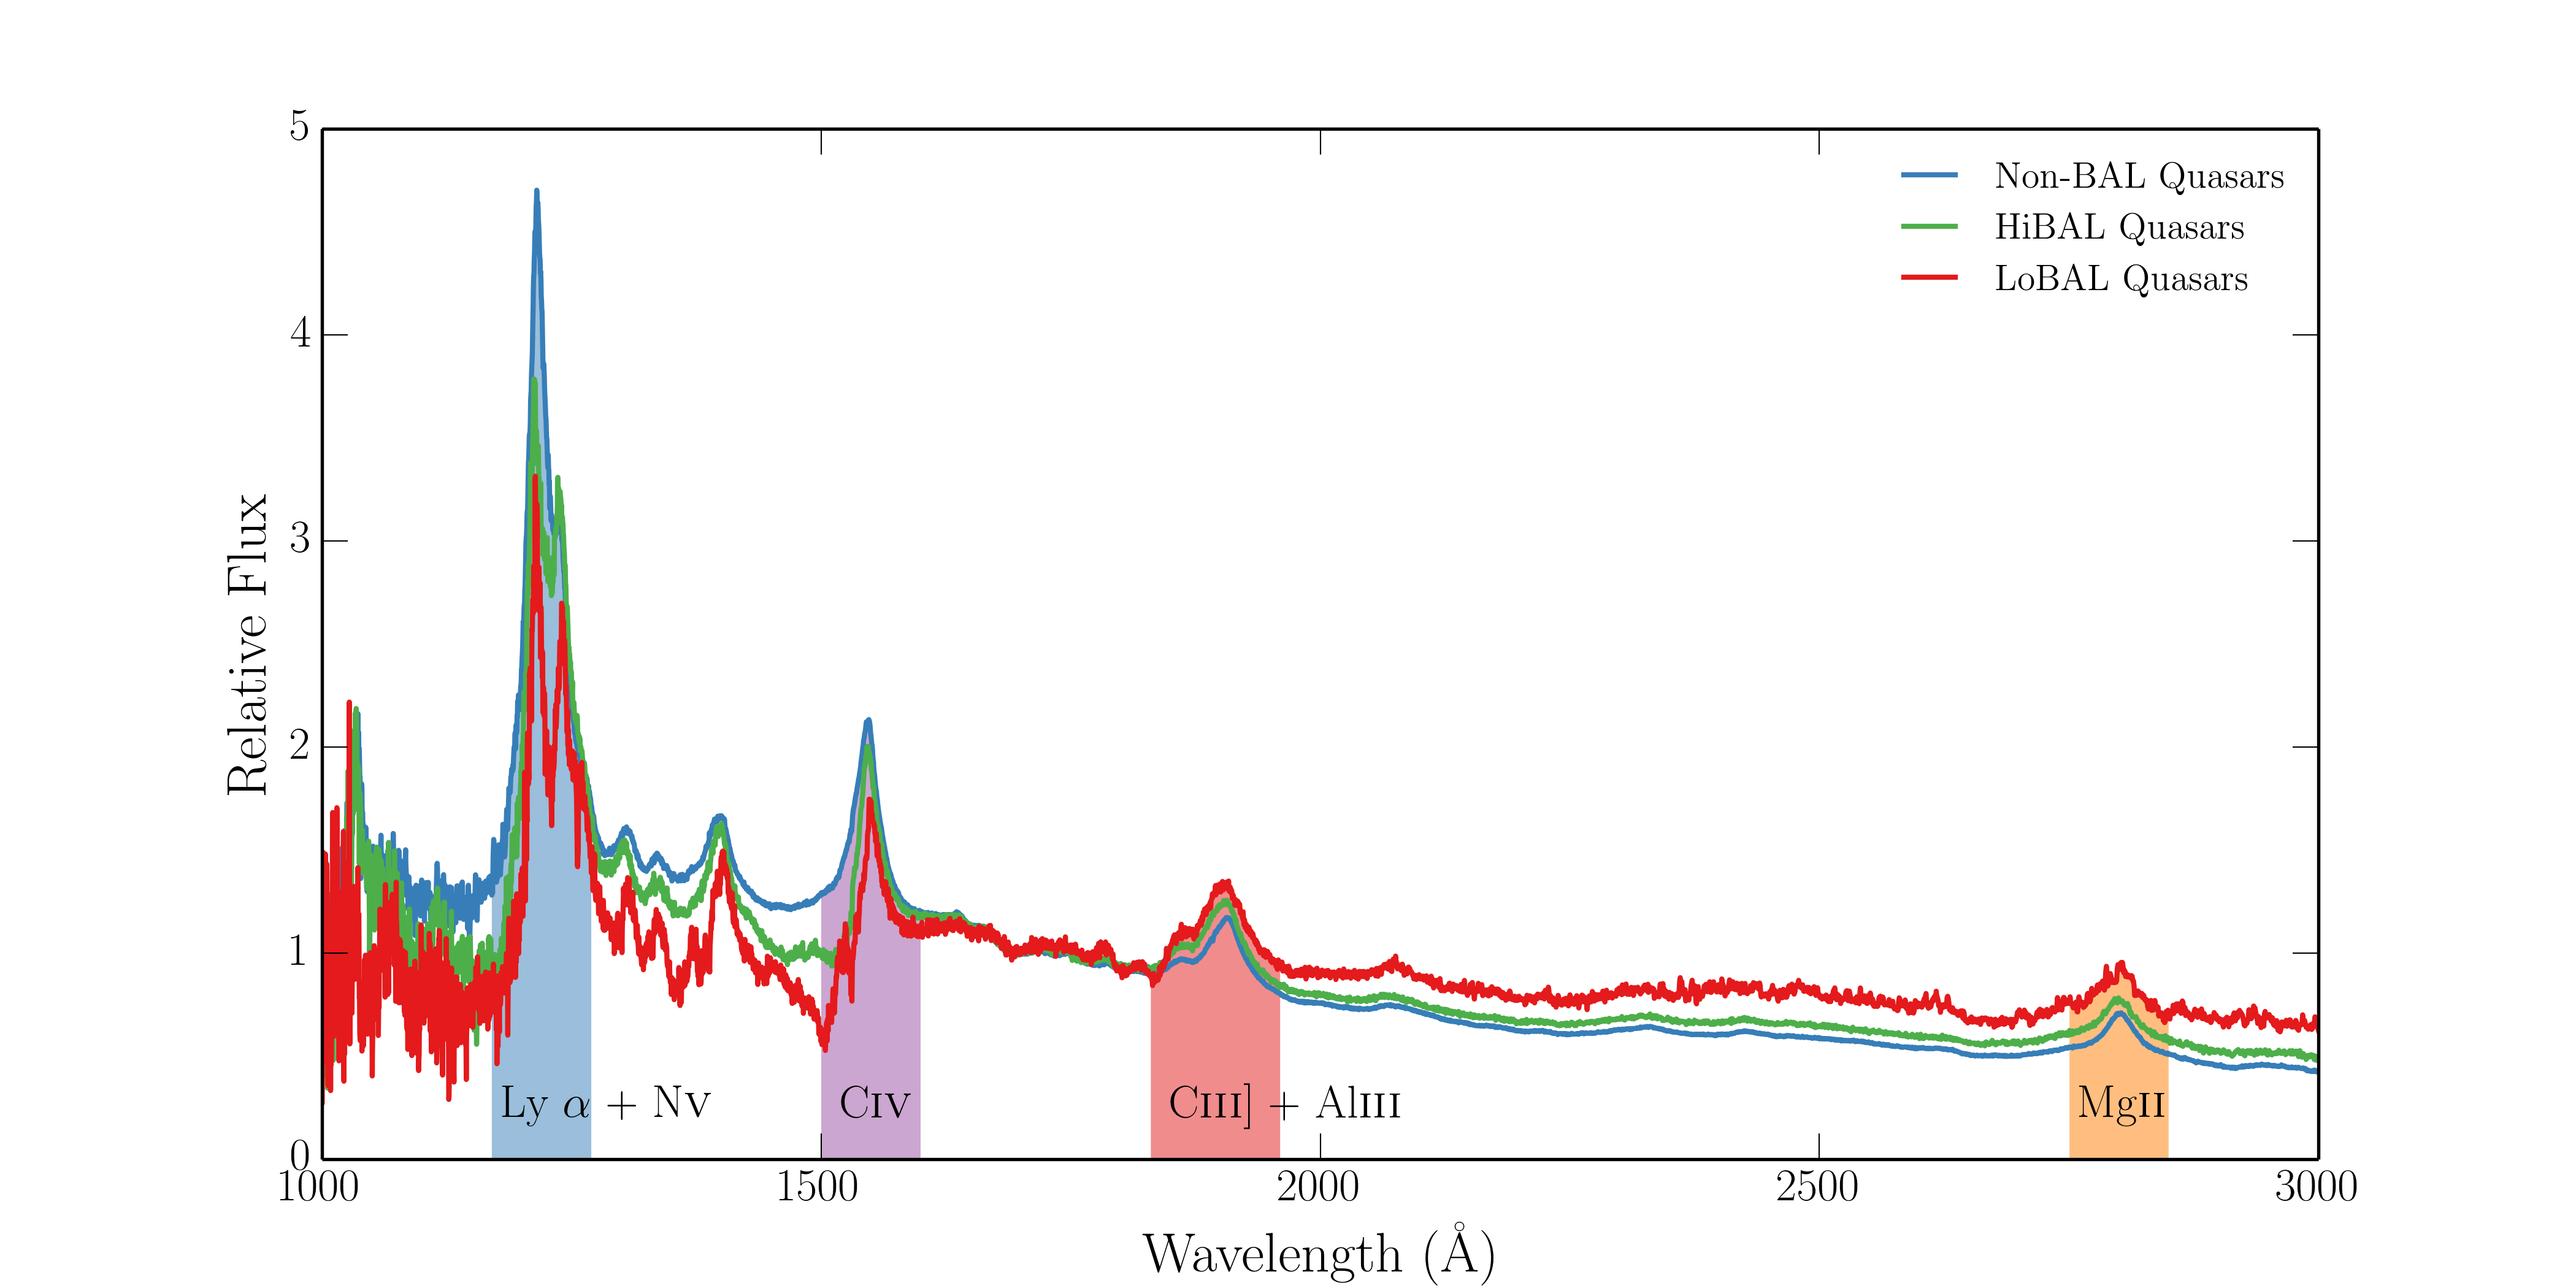
\includegraphics[width=1.0\textwidth]{figures/ewpaper/composites.png}
% \caption
% {
% SDSS Composite spectra
% }
% \label{fig:composite}
% \end{figure*} %fullpage
% The Sloan Digital Sky Survey DR7 contains ~10,000 objects in its quasar
% catalog. Many of these have been fitted with quasar templates, allowing 
% easy comparison of the equivalent width properties between the BAL and 
% non-BAL subsamples. Figure 2 shows histograms of a number of different 
% emission line properties. As found by previous authors, we find that BAL
% and non-BAL quasars really do seem to possess very similar emission line 
% properties.

% \begin{table}
% \begin{tabular}{p{2cm}p{1cm}p{1cm}p{1cm}p{1cm}}
% Sample & Redshift Range & Number of non-BAL Objects & Number of BAL objects & Number of LoBAL objects \\
% \hline \hline 
% A & $?<z<?$ & 
% \hline 
% \end{tabular}
% \caption{
% The properties of our subsamples, built from the SDSS DR7
% quasar catalog.
% }
% \label{tab:samples}
% \end{table}

\begin{figure*} %fullpage
\centering
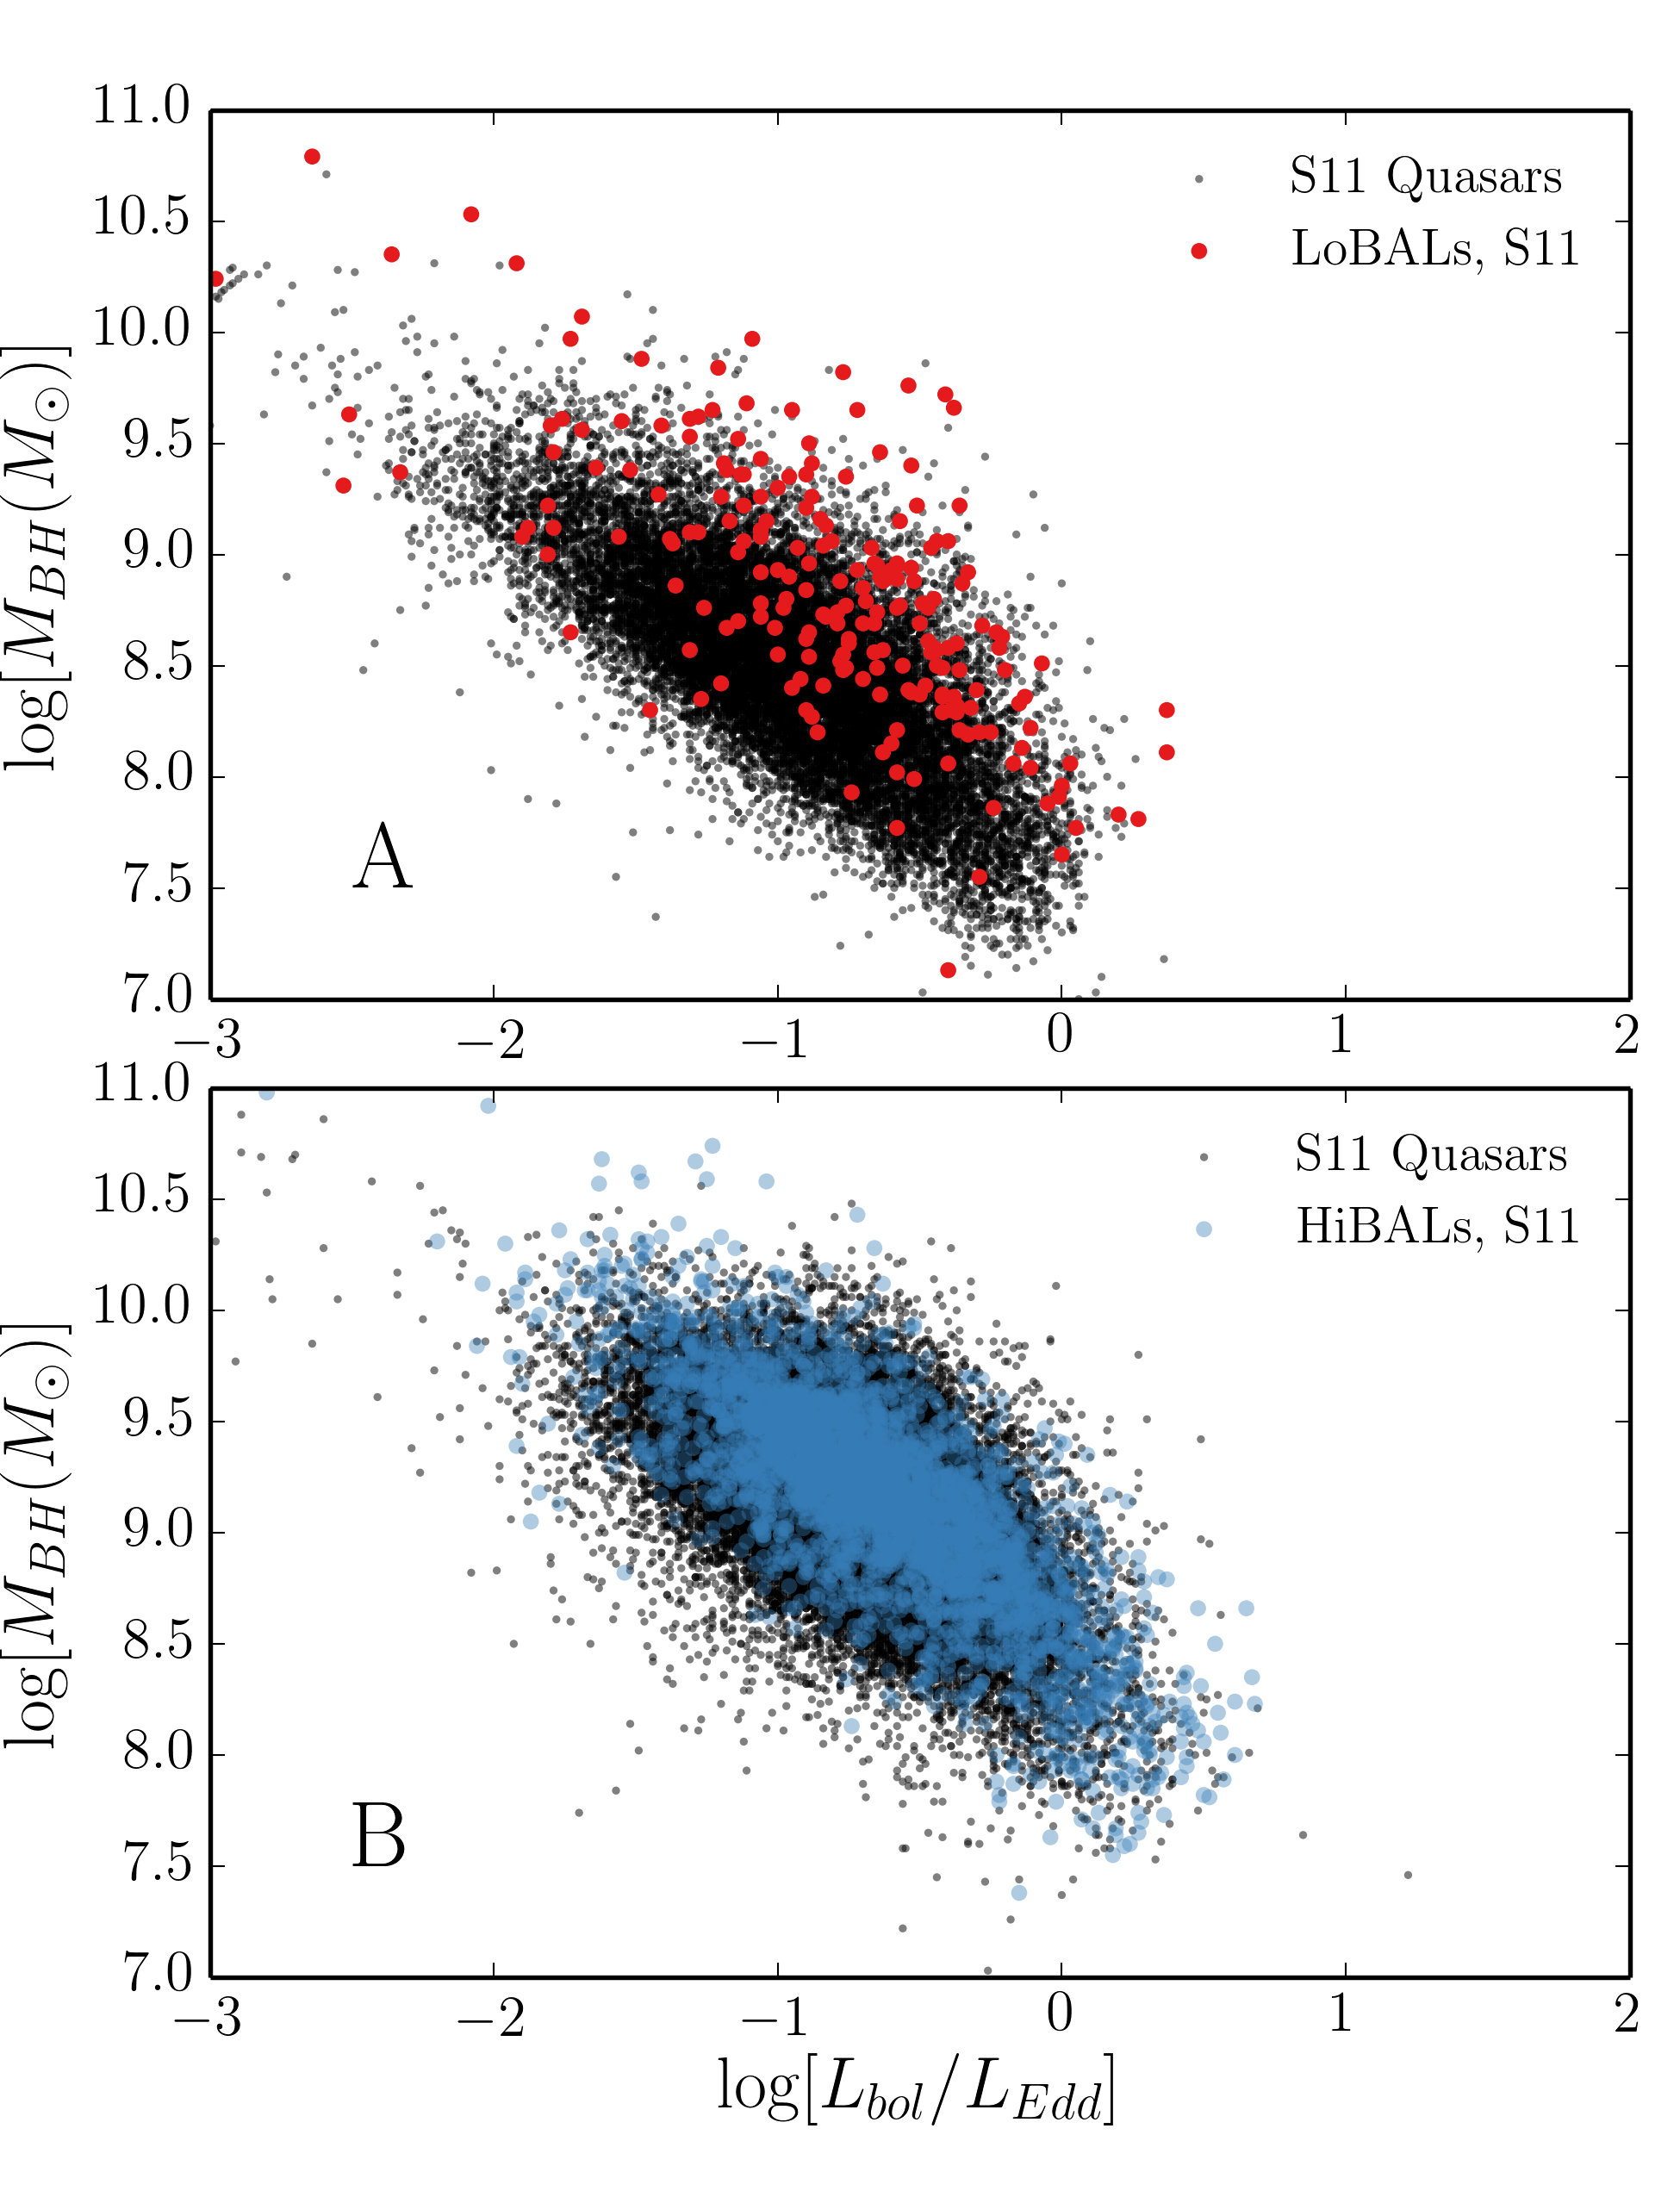
\includegraphics[width=1.0\textwidth]{figures/ewpaper/bals_2x2_scatter.png}
\caption
[BH mass and Eddington fraction measurements for samples A and B.]
{
BH mass and Eddington fraction measurements from S11 for Sample A (top)
and Sample B (bottom). The LoBALs in sample A and BALs in Sample B are
also plotted in each case.
}
\label{fig:bal_scatter}
\end{figure*} %fullpage

\begin{figure*} %fullpage
\centering
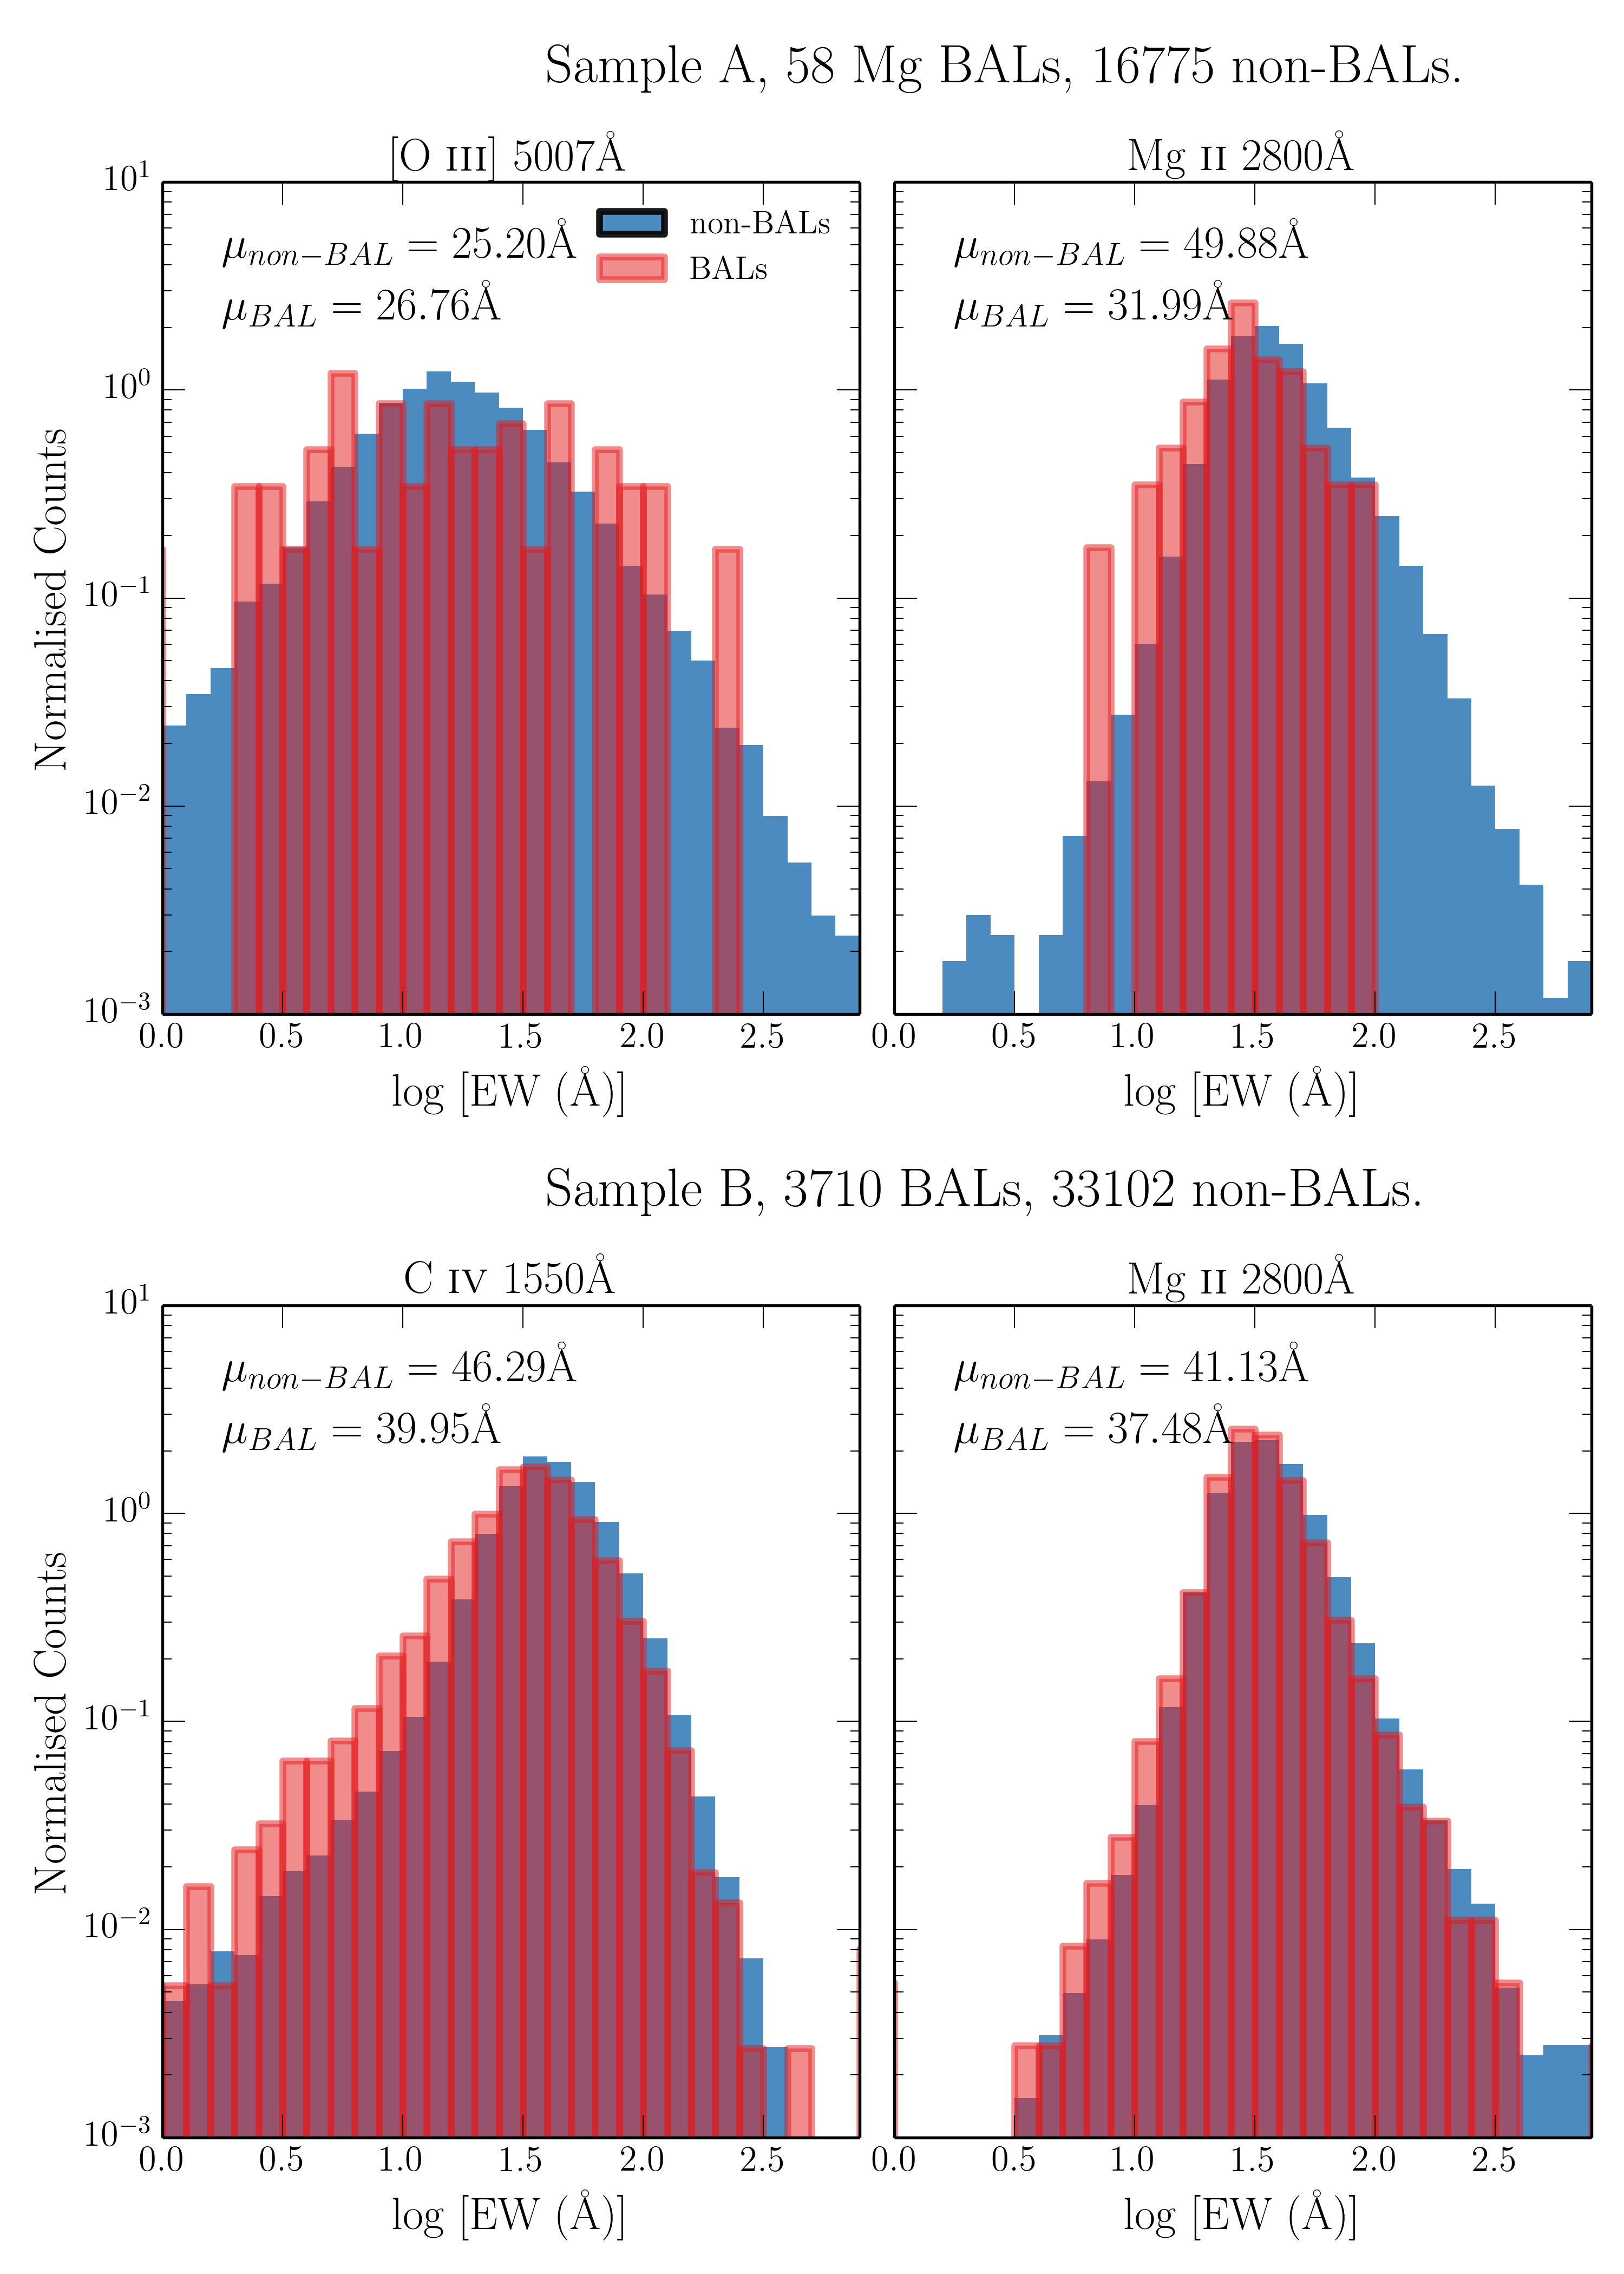
\includegraphics[width=1.0\textwidth]{figures/ewpaper/ew_hist_qsos.png}
\caption
[Histograms of equivalent widths for three emission lines from the two different samples.]
{
Histograms of equivalent widths for three emission lines from the two different samples.
The mean of the BAL and non-BAL quasar distributons are labeled in each case, and
the histograms are normalised so that they integrate to 1.
}
\label{fig:ew_hists}
\end{figure*} %fullpage

The data sample is based upon the
\citet[][hereafter S11]{shen2011} catalog of
105,783 quasars from the The Sloan Digital Sky Survey (SDSS) 
Data Release 7 (DR7). 
As I will use emission line diagnostics in this study,
this sample must be further divided according to which 
emission lines are present in 
the SDSS wavelength range at a given redshift. 
Sample A contains all quasars within the redshift range $0.35<z<0.83$, 
such that the \mgline\ and \oiiifull\ line EWs are both measured, 
and \mg\ BAL identification
is possible.  Sample B contains all quasars within the redshift 
range $1.45<z<2.28$, such that 
the EWs and presence of BAL in \mgline\ and \civline\ are both measurable.
The BH mass estimates and Eddington fraction measurements from S11 of the two samples,
are shown in Fig.~\ref{fig:bal_scatter}
against the background distribution of all S11 quasars.

S11 are careful to take into account traditional problems with quasar line fitting,
such as narrow line or Fe pseudocontinuum contamination, in their fits to 
emission line profiles and resultant EW measurements. For \mgline\
this includes careful subtraction of the Fe emission using the \cite{vestergaard2001}
templates. This subtraction is not included for \civfull,
as the Fe emission is less prominent and harder to model. This may lead to
a systematic overestimate by $\sim0.05$ dex in the \civ\ line EW. 
The \oiiifull\ line is fitted with a Gaussian. The flux ratio of this line 
with the sister component of the doublet, \oiiidoublet, is found to agree well 
with the theoretical expectation of around 3, implying a reliable subtraction of broad \hb.
In order to mask out the effects of e.g., absorption, on the \civ\ and \mg\ lines, 
S11 ignore $3\sigma$ outliers in the fit to the profile. Based on these
considerations, the S11 catalog makes for a reliable set of EW 
measurements. This is especially true when making inferences from 
multiple emission lines, as systematics inherent to individual lines 
or spectral windows are less likely to affect the analysis as a whole.

In attempting to draw broad conclusions about unification models as a whole,
I would ideally also construct a large, homogenous dataset of 
HiBAL and non-BAL quasars, both with \oiiifull\ EWs. Unfortunately,
the wavelength limits of SDSS do not allow this; only LoBAL quasars have 
both BAL and \ewo\ measurements. One of the problems with
using just LoBALQSOs in tests of unification is that there is evidence 
that they are drawn from a different population than normal quasars. 
Examples include anomalously 
high LoBAL fractions in dust-reddened quasar samples \citep{urrutia2009} 
and infra-red selected samples \citep{dai2012}; 
although see also \cite{lazarova2012}.

Fig. 2 shows histograms of a number of different 
emission line properties for samples A and B. 
As discussed by previous authors \cite[e.g.][]{weymann1991}, I find that BAL
and non-BAL quasars seem to possess very similar emission line 
properties. The EW is related to the intrinsic, `face-on' equivalent width,
$\ew_*$ by the equation
\begin{equation}
\ew = \ew_* /\epsilon(\theta)
\end{equation}
where $\theta$ is the viewing angle with respect to the symmetry axis 
and $\epsilon(\theta)$ is the `angular emissivity function', which describes 
how the continuum luminosity from the disc varies as a function of viewing angle.
For a foreshortened disc this is simply $\epsilon(\theta) = \cos \theta$. 
Note that this assumes isotropic line emission, which may not be accurate for optically thick
permitted dipole transitions; the effect of line anisotropy is discussed further 
in section~\ref{sec:line_aniso}.

If BALQSOs are preferentially viewed from larger-than-average viewing angles,
we would expect them to possess higher EWs. 
It is already apparent from Fig.~\ref{fig:ew_hists} that the BALQSO distribution means 
are not significantly higher than the non-BAL quasar
means -- in fact, in many cases they are lower. 
This is not expected from a model
in which the continuum comes from a foreshortened disc, and BAL outflows are at all equatorial.
This problem is examined further in section~\ref{sec:mc_angular}. 
First, I will examine the motivations for different forms of \ept\ 
in AGN and quasars.

\section{The Angular Distribution of Emission from an Accretion Disc}
\label{sec:disc_agn}

\noindent 
As introduced in chapter 1, the most widely-used theoretical model for accretion discs
is the so-called `$\alpha$-disc' model of SS73. 
There are a number of well-documented problems when fitting 
AGN SEDs with SS73 accretion disc models (see section~\ref{sec:disc_continuum}), 
Despite these problems, \cite{capellupo2015} succeeded
fitting $\alpha$-disc models to AGN specta when the effects of
GR, mass-loss and comptonisation were included.
In this section, I start by discussing the angular distribution of
emission from a classic SS73 disc, before exploring opacity and GR 
effects. In order to do so, I use \agn\
\citep{hubeny2000,davishubeny2006,davis2007}. I stress that the 
discussion here is not limited to $\alpha$-discs; the only real condition
for the angular distributions derived here is that the 
disc is geometrically thin and optically thick.

\subsection{Standard Thin Disc Models}

\noindent
Any geometrically thin, optically thick disc will appear
foreshortened and limb darkened (if temperature decreases
with height from the central disc plane). 
Foreshortening is a simple $\cos \theta$ geometric effect, 
where $\theta$ is the inclination with respect to the vertical z axis, which
is perpendicular to the disc plane.
Limb darkening, $\eta(\theta)$, is usually approximated by a linear dependence
of the emergent flux on $\cos \theta$, i.e. 
\begin{equation}
\eta(\theta) = a \left( 1 + b \cos \theta \right),
\end{equation}
where $a$ is a normalisation constant, and $b$ governs the strength
of the limb darkening. Setting $b=3/2$, known as the Eddington approximation,
tends to give good agreement with solar observations 
\citep[e.g.][]{mihalas}. The two effects can be 
combined to give a net angular emissivity function of
\begin{equation}
\epsilon(\theta) = a \cos \theta \left( 1 + \frac{3}{2} \cos \theta \right).
\end{equation}

\subsection{Including GR and Opacity Effects}

\begin{figure}
\centering
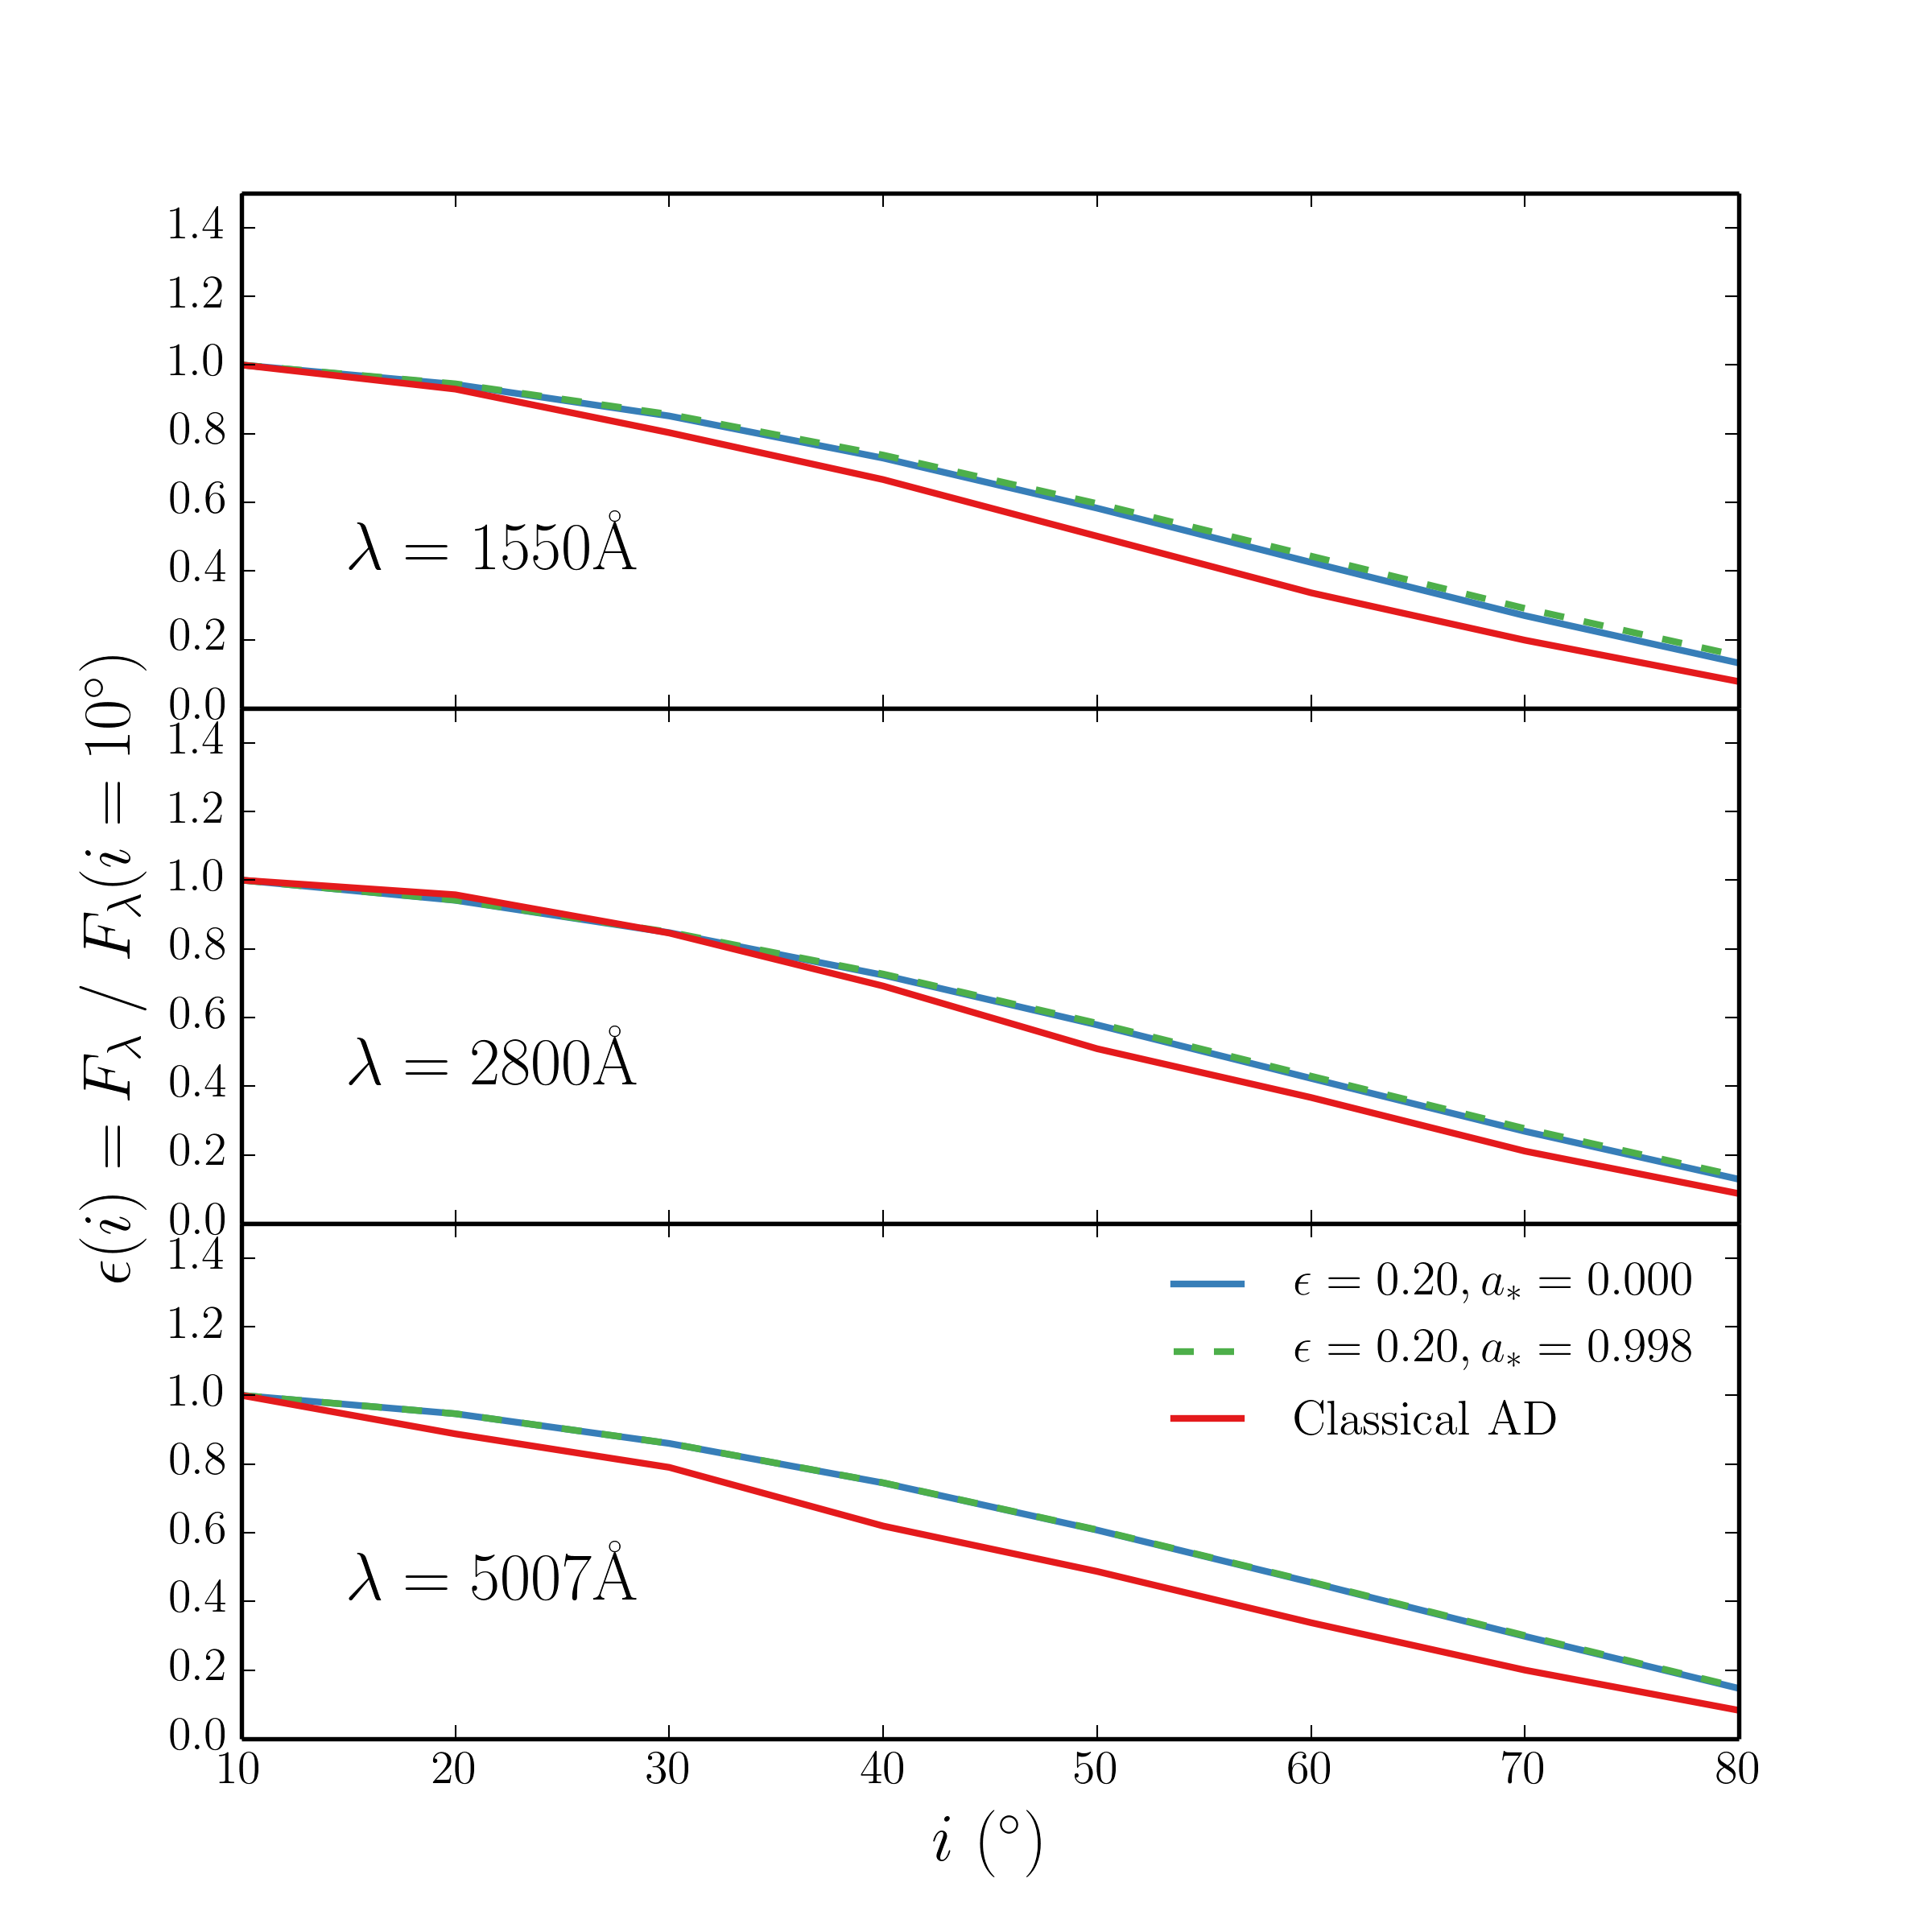
\includegraphics[width=1.0\textwidth]{figures/ewpaper/agnspec.png}
\caption
[Angular variation of continuum luminosity from \agn\ and classical thin disc models.]
{
Angular variation of continuum luminosity from \agn\ and classical thin disc models.
The monochromatic continuum luminosities is divided by the monochromatic continuum luminosity
at $10^\circ$, from \agn\ and classical thin disc models, at three different wavelengths.
The models are computed for an Eddington fraction of $0.2$ and $M_{BH}=10^9~M_\odot$. 
In each panel I show both Kerr and Schwarzschild \agn\ models, and the classical models are
for both pure foreshortened discs and foreshortened and limb darkened (LD) discs.
}
\label{fig:agnspec_disc}
\end{figure} 


\noindent
In reality, limb darkening is not frequency independent and 
depends on the bound-free and bound-bound opacities in the disc.
In addition, it has been shown that GR light bending can `isotropise' the radiation
field in XRBs \citep{zhang1997,munozdarias2013}, in some cases overcoming
foreshortening effects. In order to assess the impact of GR and disc opacities
on \ept, I use \agn\ models, which conducts a stellar atmosphere calculation
to obtain the SED from a series of annuli, before using the \kerrtrans\ code \citep{agol1997}
to calculate the emergent SED by ray-tracing along Kerr geodesics.
Fig.~\ref{fig:agnspec_disc} shows \ept\ as a function of 
$\theta$ for two \agn\ models for minimally and maximally spinning BHs. 
The models are characterised by $M_{BH}=10^9~M_\odot$ and an Eddington fraction of $0.2$.
The angular distribution is fairly insensitive to these choices.
For comparison, I also show foreshortened and limb-darkened predictions for SS73 models.
Although the \agn\ continua are significantly more isotropic at $500$~\AA,
there is very little effect redward of around $1000$~\AA, which is the relevant
region of \ept\ for \oiiifull, \civline\ and \mgline . 
In fact, using the foreshortened estimate is the conservative (least anisotropic) prescription 
in these regimes. I will thus adopt \ept$=\cos \theta$ for the remainder of this work.










\section{Predicted EW Distributions Compared to Observations}
\label{sec:mc_angular}

\subsection{Fitting the Quasar Distribution}
\label{sec:fitting}

\citet[][hereafter R11]{risaliti2011} analysed the \ewo\ 
distribution of 6029 quasars in SDSS DR5. They demonstrated
that a foreshortened disc and isotropic \oiiifull\ line produces
a high EW tail in the EW distribution, with a characteristic 
slope of $\Gamma_{EW}=-3.5$. In order to first reproduce their
result and discuss its implications, I have 
created a sample according to their selection
criteria. The criteria are that the object in question lies in the redshift
range 0.01 to 0.8, have an absolute magnitude $M_i>22$, an 
apparent magnitude $m_i>19.1$, and signal to noise per pixel of greater
than 5. Using the updated SDSS quasar sample of S11, this defines
a sample of 14,424 quasars.

To fit the distribution, I conduct the following procedure,
which is similar to the method R11 use to demonstrate that the power
law tail is expected.
\begin{enumerate}
	\setlength\itemsep{1em}
	\item A set of isotropic angles is chosen such that 
	$P(\theta)\propto d\Omega(\theta)$. 
	If $\theta<\theta_{1}$ then the fake object is designated as unobscured, 
	and otherwise the object is ignored. 
	\item To be included in the sample, the object also has to 
	survive a selection test
	to simulate the distribution of angles in a flux-limited sample.
	This is done by drawing a random sample from the real quasar sample, 
	and calculating a `doubly observed continuum flux', $F_O$ at $5100$~\AA\ 
	(rest frame), such that $F_O = F_{5100}~\epsilon(\theta)$. The flux limit
	is set at $5\times10^{-13}$~erg~s$^{-1}$~cm$^{-1}$~\AA$^{-1}$, but the results
	are fairly insensitive to the limit chosen.
	\item For each mock sample, an EW$_*$ is drawn from an intrinsic 
	(i.e. `face-on') EW distribution for quasars. This is assumed to be a
	Gaussian distribution. The mean, $\mu_*$, and width, $\sigma_*$, of this Gaussian
	can either be set arbitrarily -- for example, to demonstrate trends
	in mock data -- or obtained from a $\chi^2$ fit to the observed EW
	distribution.
	\item A mock EW is estimated such that $\ew = \ew_* / \epsilon(\theta)$,
	and this process is repeated to build up a mock sample of $10^6$ objects.
\end{enumerate}
The result of this numerical experiment is, as found by R11, a distribution
with a high EW tail of slope $-3.5$. I can now vary the maximum angle, $\theta_1$,
and examine how this tail changes. Mock data for a series
of maximum angles is shown in Fig.~\ref{fig:cutoff}, for two different intrinsic 
Gaussians. The power law behaviour is only seen when the maximum angle is
sufficiently large, and a rapid decay in the distribution is observed
at a characteristic EW related to both the width and mean of the
intrinsic distribution as well as the cosine of the maximum angle.
The top panel has $\mu_*$ and $\sigma_*$ of the R11 Model 1, 
whereas the bottom panel shows a narrower distribution to illustrate the 
earlier onset of the high EW cutoff. 

\begin{figure}
\centering
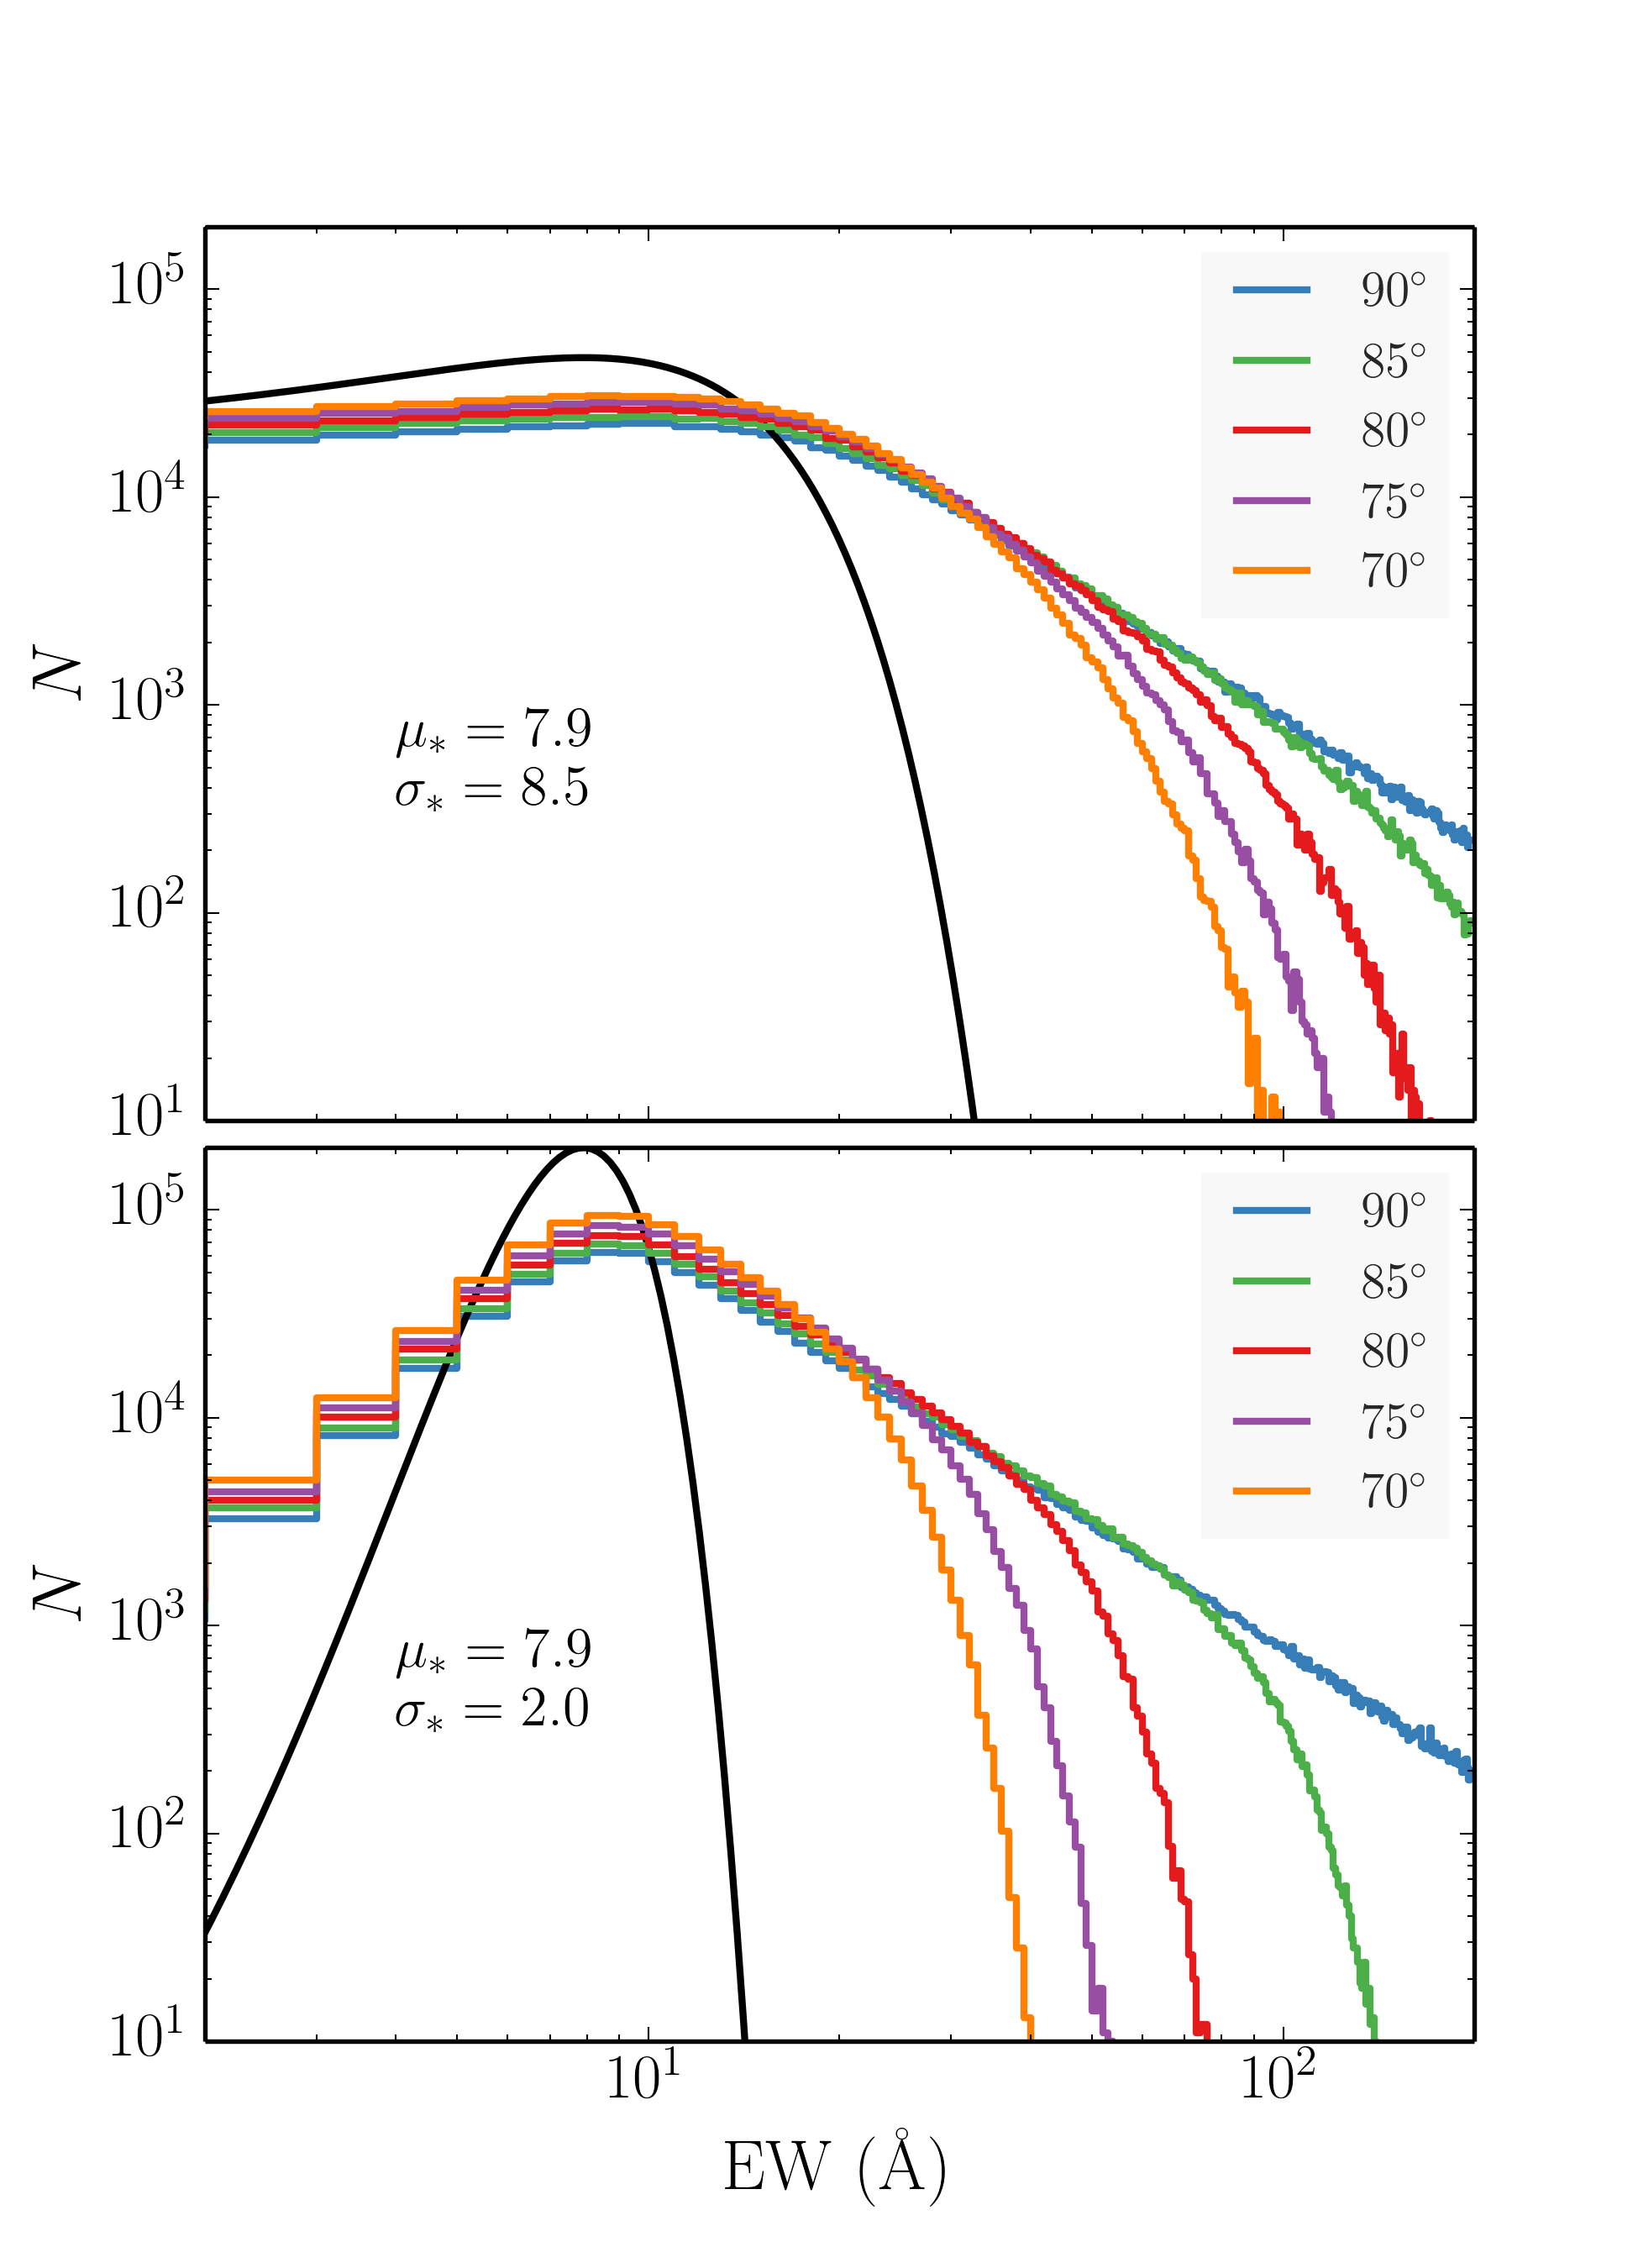
\includegraphics[width=1.0\textwidth]{figures/ewpaper/cutoff.png}
\caption
[Theoretical EW distributions from the numerical experiment 
described in section~\ref{sec:fitting}.]
{
Theoretical EW distributions from the numerical experiment 
described in section~\ref{sec:fitting} for a few different 
maximum angles. The results in the top panel use the same intrinsic
distribution as Model 1 from R11 (shown in black), 
whereas the bottom panel shows the distributions 
obtained from a narrower intrinsic Gaussian. By the time the maximum
angle is limited to around $70^\circ$ the cutoff is
clear even at moderate values of EW.
}
\label{fig:cutoff}
\end{figure}

Fig.~\ref{fig:chi2} shows the result of a $\chi^2$ minimization fit 
to the R11 sample. The best fit is achieved with a maximum angle of 
$\theta_{1}=83.5^\circ(^{+0.7}_{-0.2}, 3\sigma)$ and a narrower intrinsic distribution
than model 1 of R11. The run of $\chi^2$ with maximum angle
is shown in Fig.~\ref{fig:chi2_curve}, where the choice for $\mu_*$
and $\sigma_*$ is left free in each case. 
Maximum angles below $\sim80^\circ$ are strongly disfavoured
by this model. I adopt linear binning to facilitate easy comparison 
with R11, and only fit up $\ew=100$~\AA\
due to poor statistics above that limit. This 
makes inferring any information about a potential high EW cutoff 
difficult as a more complete sample at high EW is required. 

\begin{figure}
\centering
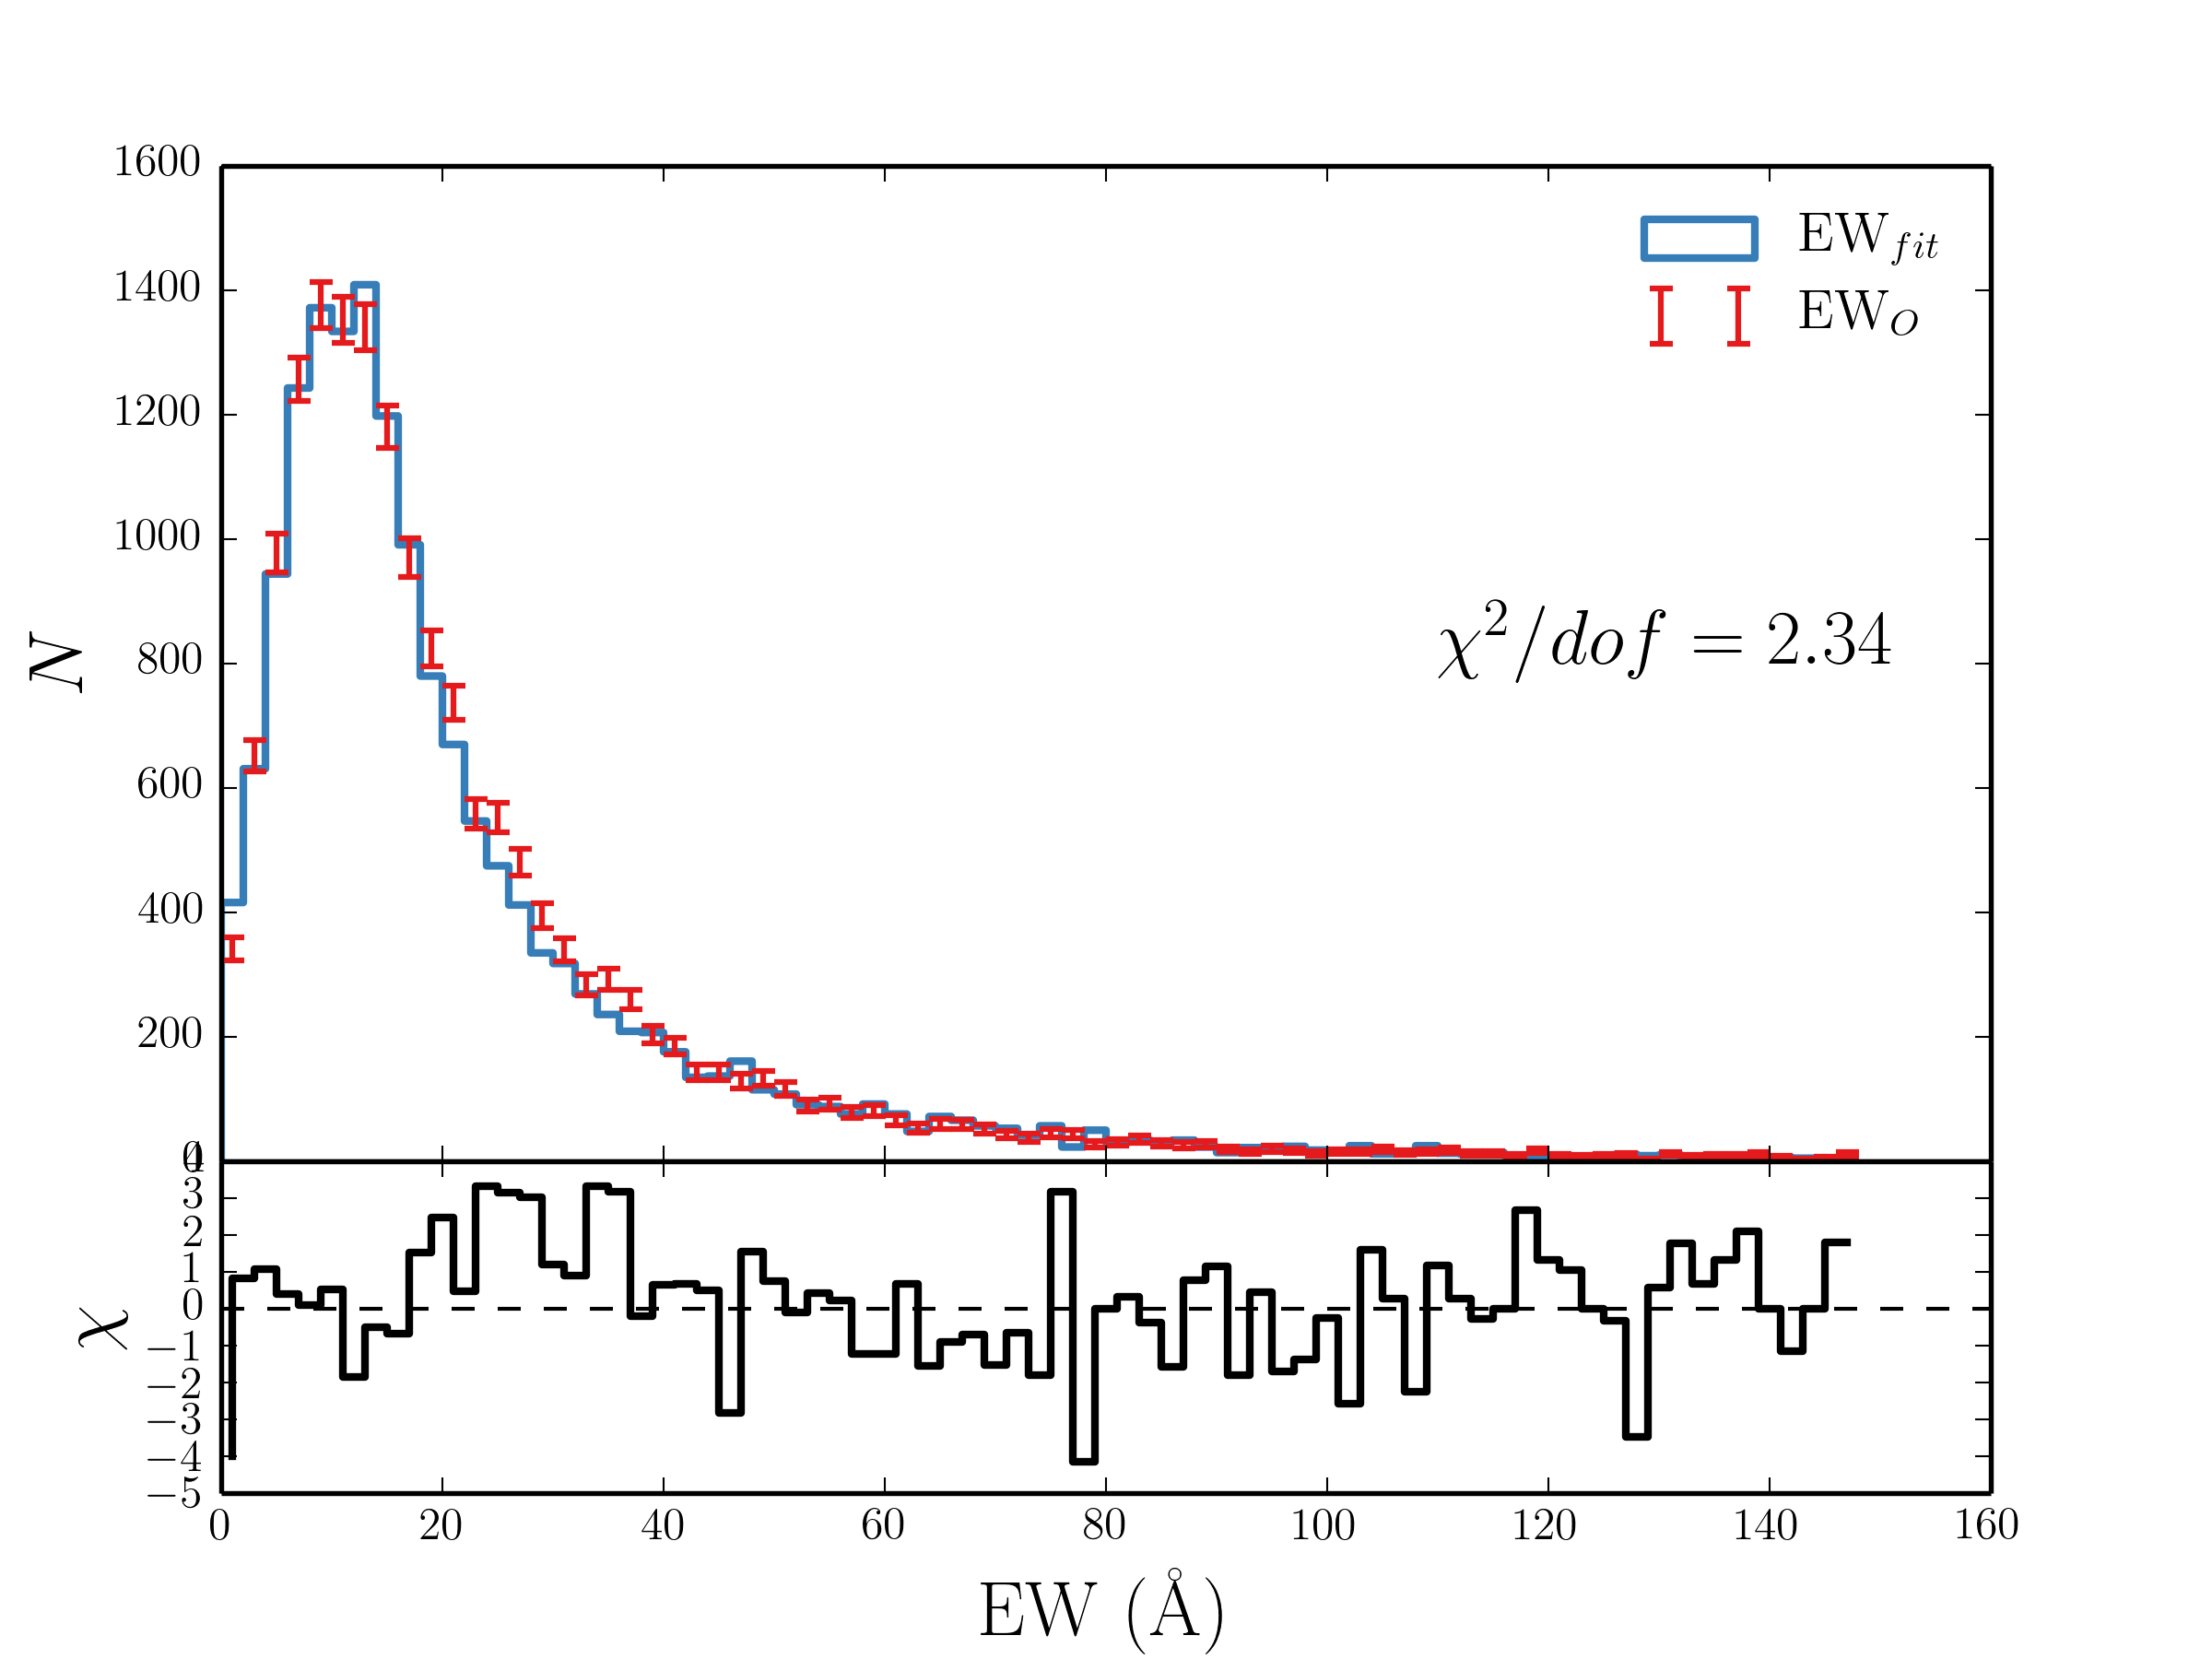
\includegraphics[width=1.0\textwidth]{figures/ewpaper/quasar_fit.png}
\caption
[The \ewo\ distribution of quasars in the R11 sample and the best fit model.]
{
The \ewo\ distribution of quasars in the R11 sample (black points), 
with $\sqrt{N}$ errorbars, and the best fit model with a maximum 
viewing angle of $84^\circ$. The intrinsic Gaussian distribution
is shown with a dashed line. The plotted data is equivalent to the non-BAL histogram 
in the top left panel of Fig.~\ref{fig:ew_hists}, except that it uses linear binning
and adopts the R11 sample criteria rather than using sample A.
}
\label{fig:chi2}
\end{figure}

\begin{figure}
\centering
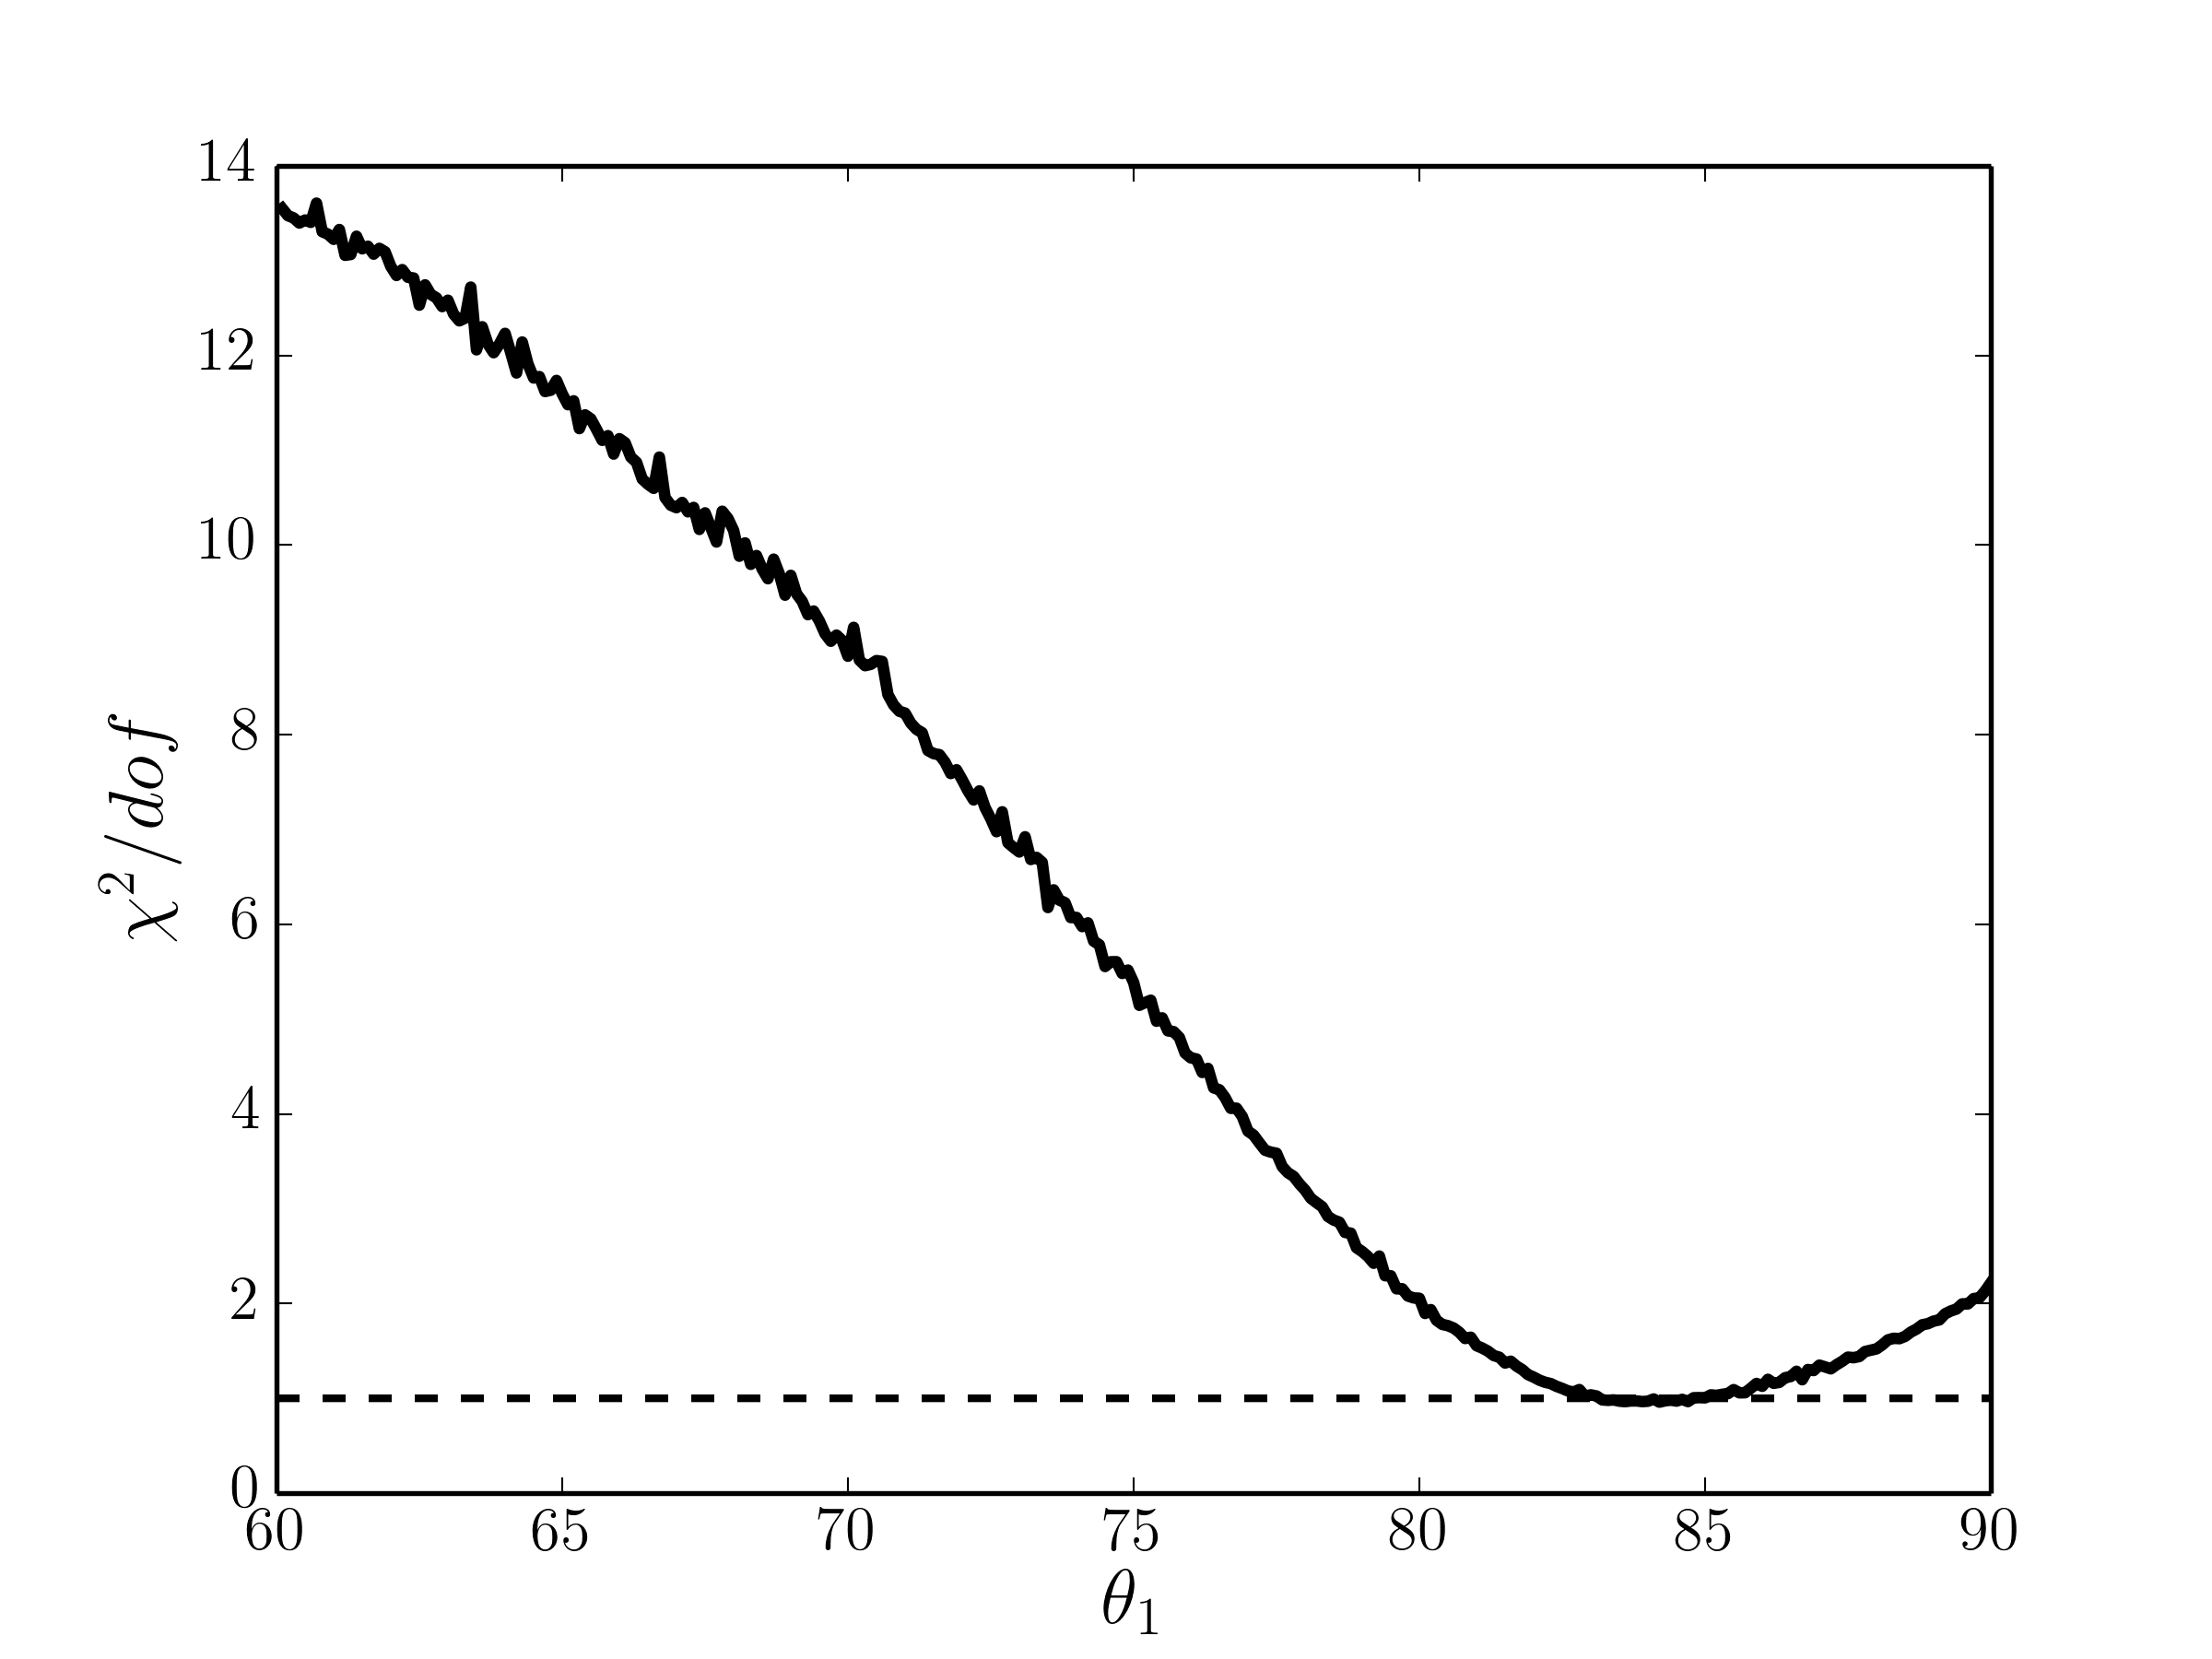
\includegraphics[width=0.8\textwidth]{figures/ewpaper/chi2_o3.png}
\caption
[$\chi^2/dof$ as a function of maximum angle.]
{
$\chi^2/dof$ as a function of maximum angle, $\theta_1$, calculated in
steps of $0.1^\circ$. The choice for $\mu_*$ and $\sigma_*$ is 
left free in each case.
}
\label{fig:chi2_curve}
\end{figure}

\subsection{Comparing non-BAL and LoBAL Distributions: Sample A}
\label{sec:bal_v_nonbal}

\begin{figure}
\centering
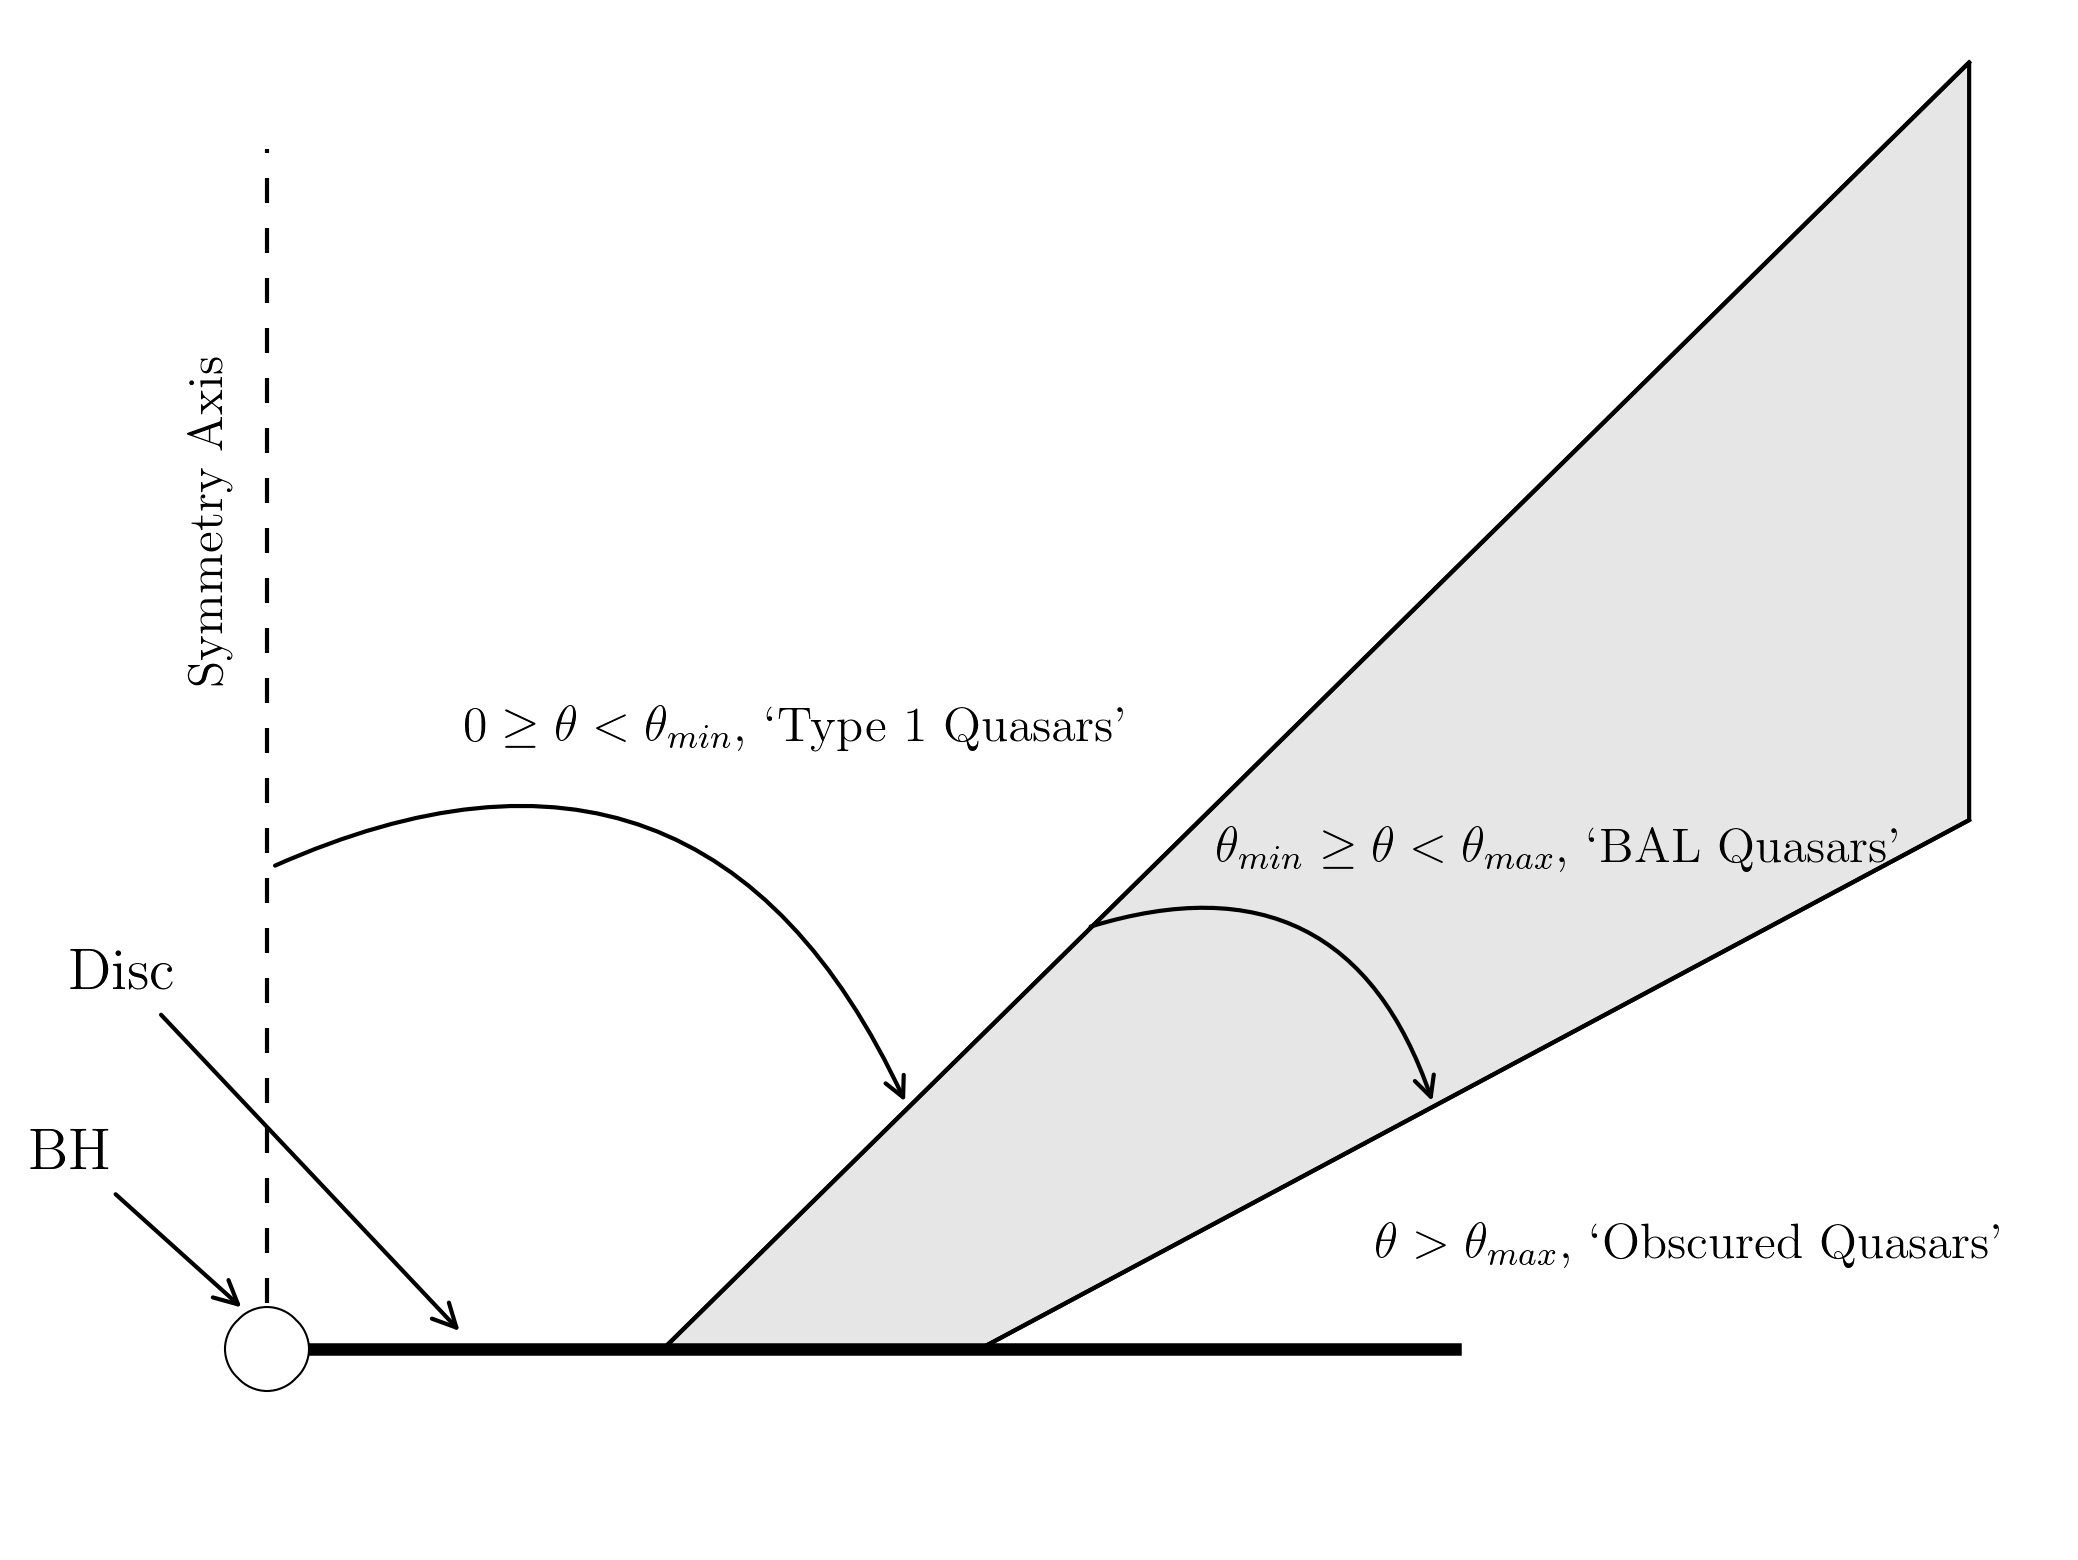
\includegraphics[width=0.8\textwidth]{figures/ewpaper/fig2_cartoon.png}
\caption
{
The geometry of the toy model used to carry out the Monte Carlo simulations.
}
\label{fig:cartoon}
\end{figure}

In order to compare the observed distributions to those expected for LoBALs and
non-BALs I conduct a Monte Carlo simulation similar to
the process described in section~\ref{sec:fitting}, but with a few 
key differences. I once again assume $\epsilon(\theta) = \cos \theta$.
The geometry of the toy model used in this simulation is shown in
Fig.~\ref{fig:cartoon}.

First, A set of isotropic angles is generated.
If $\theta_{\mathrm{min}}<\theta<\theta_{\mathrm{max}}$ then the fake object 
is flagged as a mock BAL. If $\theta<\theta_{\mathrm{min}}$ then the 
fake object is designated a non-BAL, and otherwise
the object is ignored. Once again, the object also has to 
survive a selection test based on a arbitrary flux selection limit.
I then fit the non-BAL distribution using the method described previously.
For each mock sample, a $\ew_*$ is drawn from the intrinsic gaussian,
and a mock EW is estimated such that $\ew = \ew_* / \epsilon(\theta)$.
This process is repeated to build up a mock sample of objects, and 
carried out for a series of pairs of $\theta_{\mathrm{min}}$ and $\theta_{\mathrm{max}}$.
This allows theoretical distributions for BAL and non-BAL quasars
for a series of different outflow geometries to be derived.

The diagnostics recorded from the simulation are the following four
quantities:
\begin{itemize}
	\item The $p$-value associated with a two-tailed Kolgomorov-Smirnov (K-S) 
	test statistic, $p_{KS}$, in which the mock BAL sample is compared
	to the real LoBAL sample. This is not an optimized fit parameter, but rather a measure of
	the difference between the predicted BAL data and the observed BAL data. 
	\item The BAL fraction, $f_{BAL}$, is calculated from the 
	number of objects in the mock sample with $\theta_{\mathrm{min}}<\theta<\theta_{\mathrm{max}}$.
	This is the predicted observed BAL fraction with flux selection effects, so should be compared
	directly to the `intrinsic' values of, e.g., \cite{knigge2008} and \cite{allen2011}.
	\item The $\chi^2/dof$ from the fit to the non-BAL quasar distribution.
	\item $\Delta \mu_{EW}$, the difference between the mean value of the mock BAL
	distribution and the mean value of the mock non-BAL distribution. To mimic observations,
	this should be small.
\end{itemize}
The simulation results are shown in figure~\ref{fig:contour}, in which the 
four diagnostics are plotted as a function of $\theta_{\mathrm{min}}$ 
and $\theta_{\mathrm{max}}$. 

\begin{figure*} %fullpage
\centering
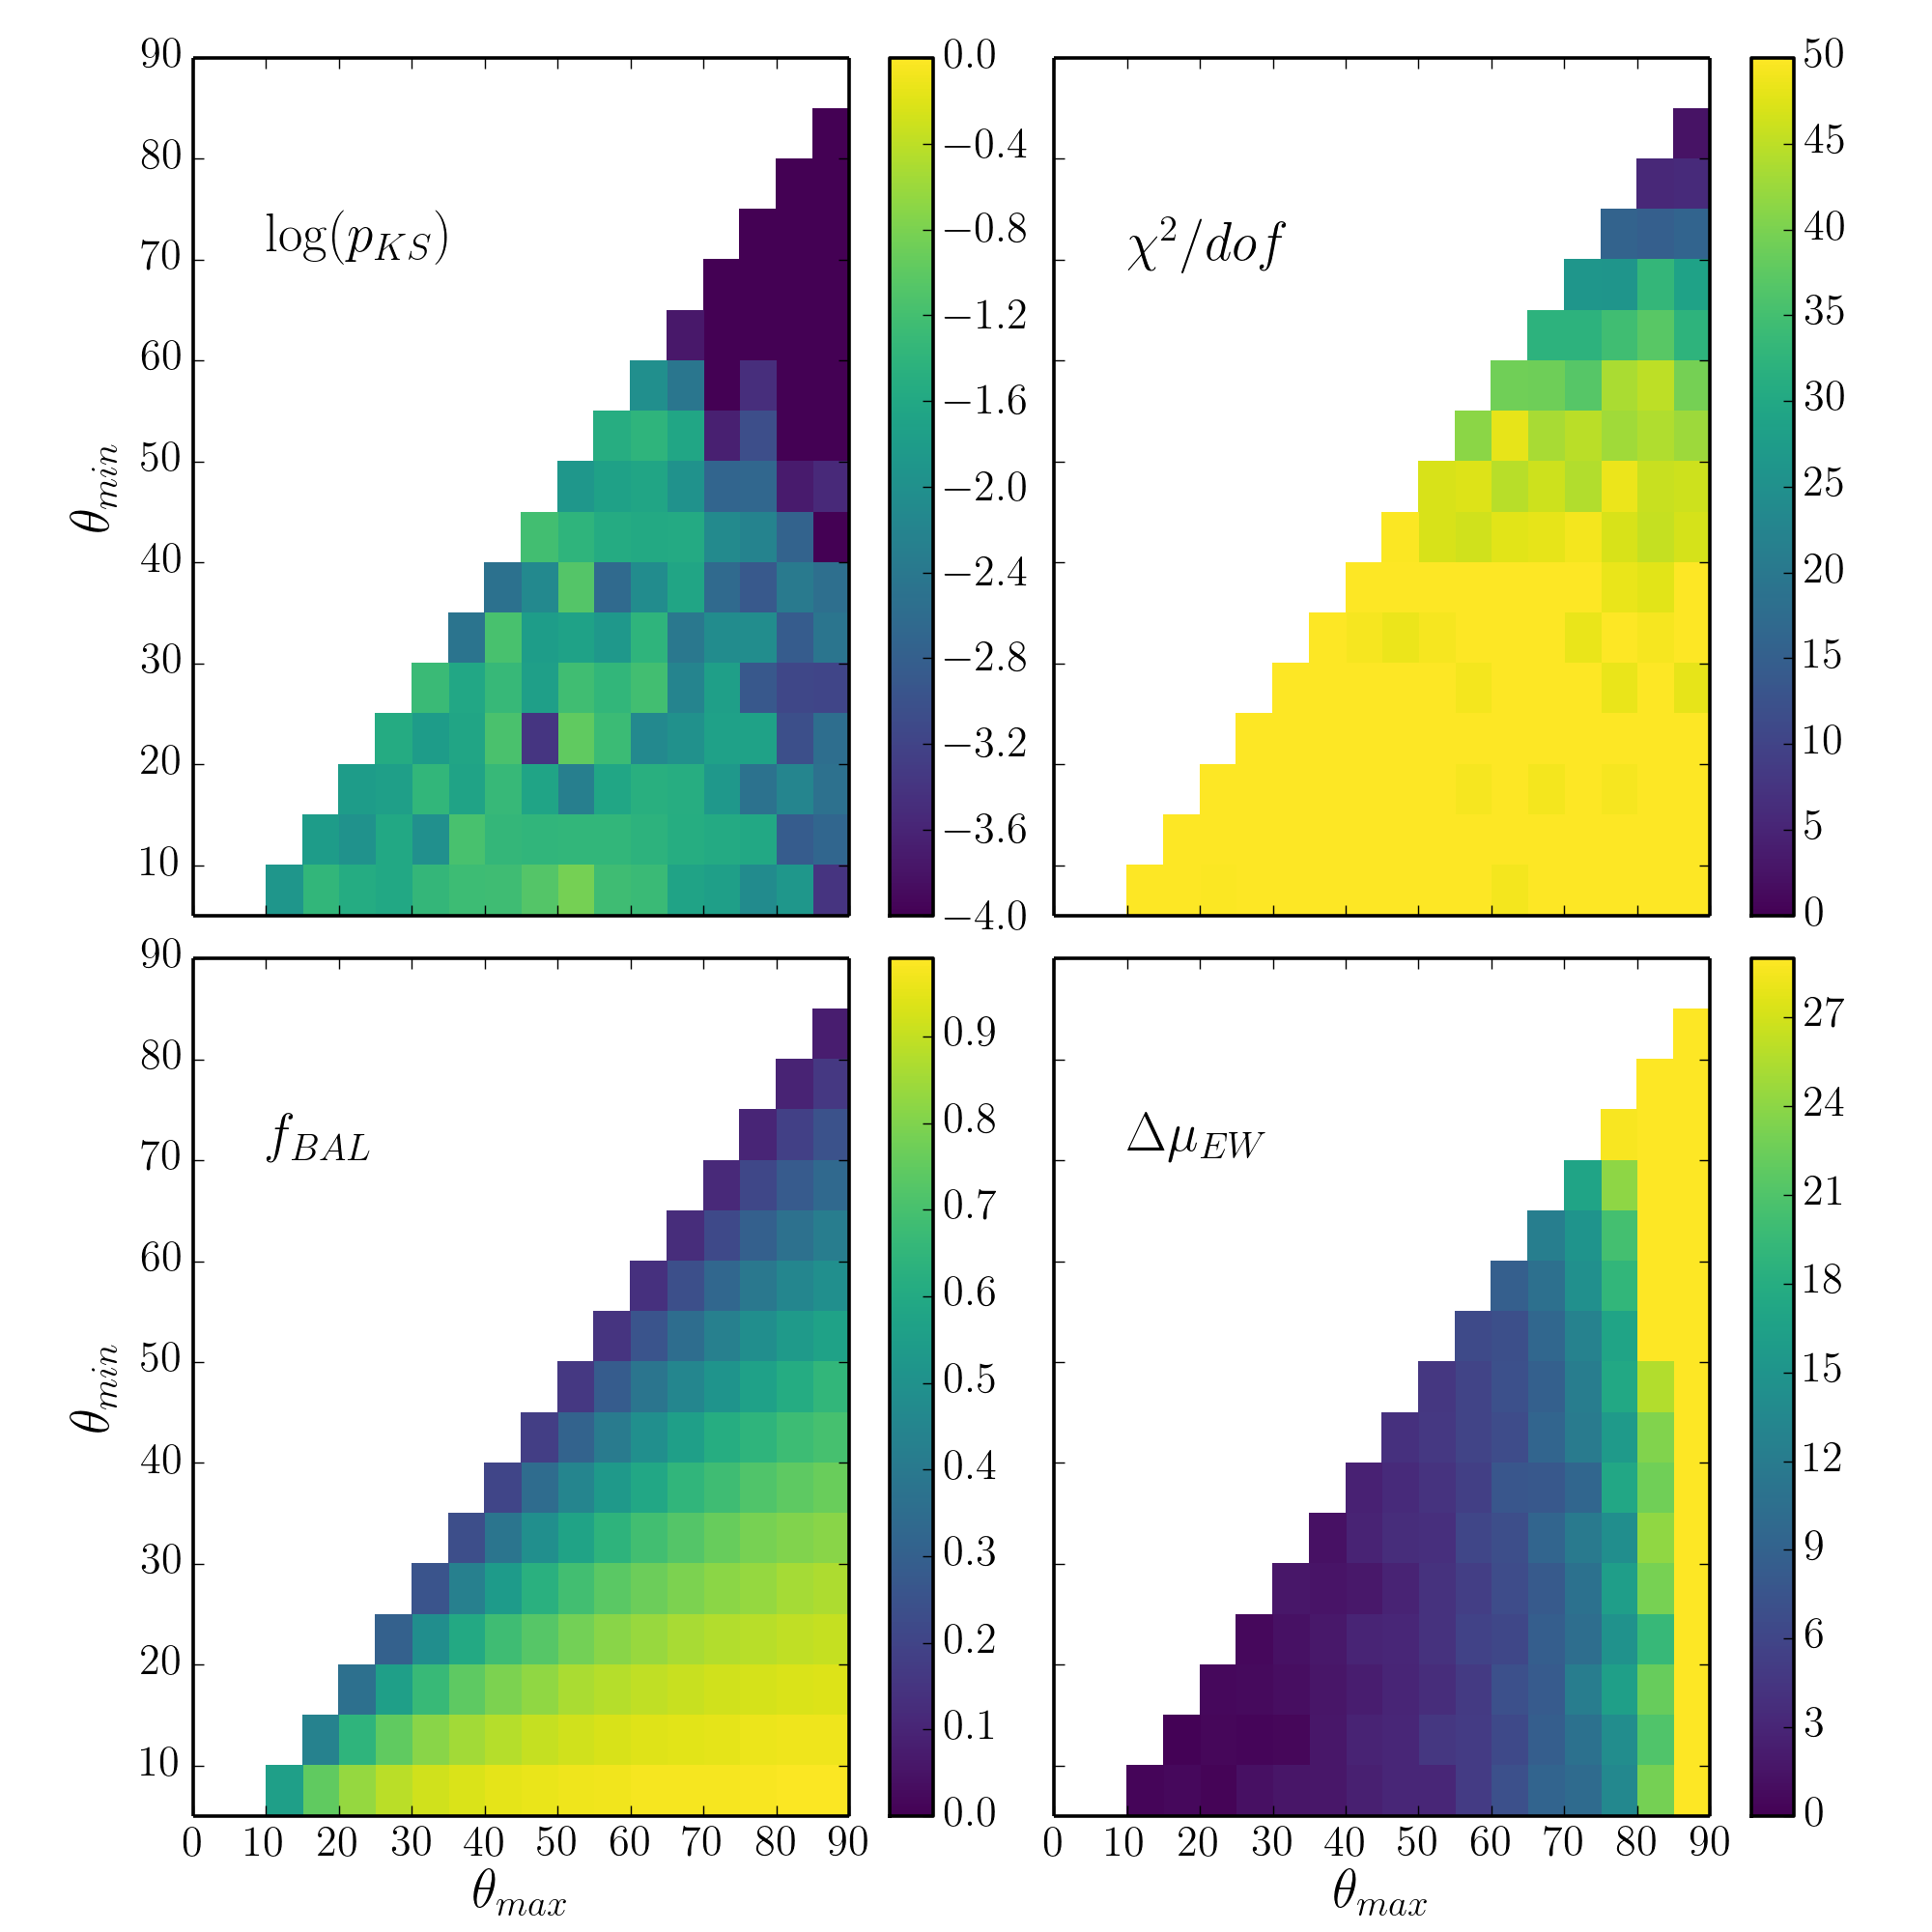
\includegraphics[width=1.0\textwidth]{figures/ewpaper/mesh4_ew_o3_max_sdss.png}
\caption
[Heat map showing the results of the MC simulation described in 
section~\ref{sec:bal_v_nonbal}.]
{
Heat map showing the results of the MC simulation described in 
section~\ref{sec:bal_v_nonbal}. The quantities shown are discussed 
further in the text, but correspond to (clockwise from top left):
the $p_{KS}$ value from a comparison between the mock BAL dataset
and the observed BAL dataset, the reduced $\chi^2$ from the fit to
the non-BAL EW distribution, the difference in mean EW between the 
mock BAL and mock non-BAL datasets, and the BAL fraction expected
for the geometry in question.
}
\label{fig:contour}
\end{figure*} %fullpage

As expected, equatorial viewing angles for LoBAL quasars 
are disfavoured, and furthermore, it is only possible to fit
the tail to the \ewo\ distribution if non-BAL quasars are allowed 
to be viewed from high inclinations. There is no region of parameter
space where a satisfactory fit is obtained to the quasar distribution
without simultaneously obtaining a large value of $\Delta \mu_{EW}$, or similarly,
a very small value of $p_{KS}$. The simulations clearly favour a geometry in which 
BALQSOs are viewed from similar angles to non-BAL quasars.

One concern with the approach used here is that systematic differences between the
non-BAL and LoBAL quasar populations in the {\em luminosity} of the \oiiifull\ line 
and continuum could mask the expected trends in \ewo. I have verified that this is a 
small effect; although \cite{boroson1992} found weak \oiiifull\ emission in LoBALQSOs,
the distributions of $L[\mathrm{\oiii}]$ are very similar in sample A. 
The LoBALQSO sample has continuum luminosities a factor $\approx2$ higher than the
non-BAL quasar sample on average -- this is not enough to
permit high inclination models, although it does moderate the conclusions slightly.

The conclusions here are also limited by the lack of knowledge about the 
intrinsic face-on distribution of \ewo, or equivalently,
the orientations of the quasars themselves. If either of these
quantities were known then the results of the
K-S test and $\chi^2$ minimization could be used
to place more robust constraints on BAL and non-BAL viewing angles 
and the associated covering factor of the outflow.
Furthermore, the distribution of \civ\ quasar EW cannot be fit by 
the same model as the \ewo\ distribution.
Another key limitation is the SDSS wavelength coverage,
which means that only LoBALs can be used when \ewo\ is present (sample A).
I would suggest that future observational programs might 
look to build up a large sample of \ewo\ measurements for HiBAL
quasars. 
% In the mean time, I will turn to the UV broad emission
% lines to examine if the above conclusions also hold
% when examining the properties of the HiBAL quasars in sample B.










\section{Discussion}
\label{sec:discuss_ew}
I have demonstrated that the EW distributions of the 
\oiiifull\ emission line in LoBAL and non-BAL
quasars is not consistent with a 
model in which LoBAL quasars are viewed from equatorial angles 
and the continuum emission originates from
a foreshortened accretion disc. The EW distributions of 
\civline\ suggest that a similar conclusion applies to HiBAL quasars.
This result would only be strengthened were 
I to include limb darkening. I will now explore how the above results compare to other
observations of quasars that might probe system orientation, as 
well as the potential impact of obscuration and line anisotropy
on the results.

\subsection{Eigenvector 1}

Eigenvector 1 (EV1) is a fundamental parameter space for AGN and quasars
\citep{borosongreen,sulentic2000ev1,marziani2001,shenho2014}. 
It relates the FWHM of \hb, the relative iron strength, 
$R_{{\rm Fe \textsc{ii}}}$, and
\ewo. Both \ewo\ and \fwh\ have been used as orientation
indicators, and so comparing the LoBALQSO EV1 distribution to the non-BAL 
quasar EV1 distribution is particularly interesting. Once again,
HiBALs cannot be placed on this space due to the lack of rest-frame 
optical coverage.

Fig.~\ref{fig:bal_ev1} shows the quasar distribution from sample A 
in EV1 parameter space, with LoBAL quasars from sample A overplotted.
\citet[][hereafter SH14]{shenho2014} propose 
that the main inclination driver in this parameter space
is \fwh, and that high inclination sources should thus cluster around
a diagonal line from the lower right to upper left quadrants. In contrast,
R11's analysis predicts that high inclination sources should cluster
around high EW OIII widths. As \ewo\ and \fwh\ are very weakly correlated
(Spearman's rank coefficient of 0.14), this means they should lie to
the left of the parameter space. Inspection of the figure clearly 
shows that BAL quasars are not only found in one region of the 
EV1 parameter space. 

In order to assess this more quantitatively, I also show contours of 
quasar counts overlaid on the scatter plot. The contours correspond
to the number of objects in each bin, where the bins are of size
$\Delta R_{{\rm Fe \textsc{ii}}} = 0.2$ and $\Delta$\fwh$=500$km~s$^{-1}$.
The percentage of quasars falling within the inner contour is 45\%, 
whereas only 18\% of LoBALQSOs fall in the space. Conversely, 24\% 
of LoBALQSOs fall outside the outermost contour compared to 10\% of 
non-BAL quasars. It would therefore appear that BAL 
quasars are preferentially clustered towards the high-mass and 
high-inclination end of EV1 space (under the interpretation of SH14).
This is further illustrated by Fig.~\ref{fig:bal_ev1_bins},
which shows the LoBAL fraction in larger bins, compared to the 
mean LoBAL fraction. This is again suggestive of an overdensity of LoBALQSOs 
towards the upper right of the parameter space.
It is also clear that a unification picture in which BAL 
quasars are viewed exclusively from high inclinations is 
inconsistent both the R11 and SH14 interpretations. 

Larger datasets, preferably including HiBAL quasars with EV1 measurements, 
are needed in order to properly constrain the EV1 behaviour of BAL quasars.
However, overall, the behaviour of EV1 in LoBALQSOs slightly 
strengthens the conclusion that BAL quasars are not always viewed from 
extreme inclinations.

\begin{figure}
\centering
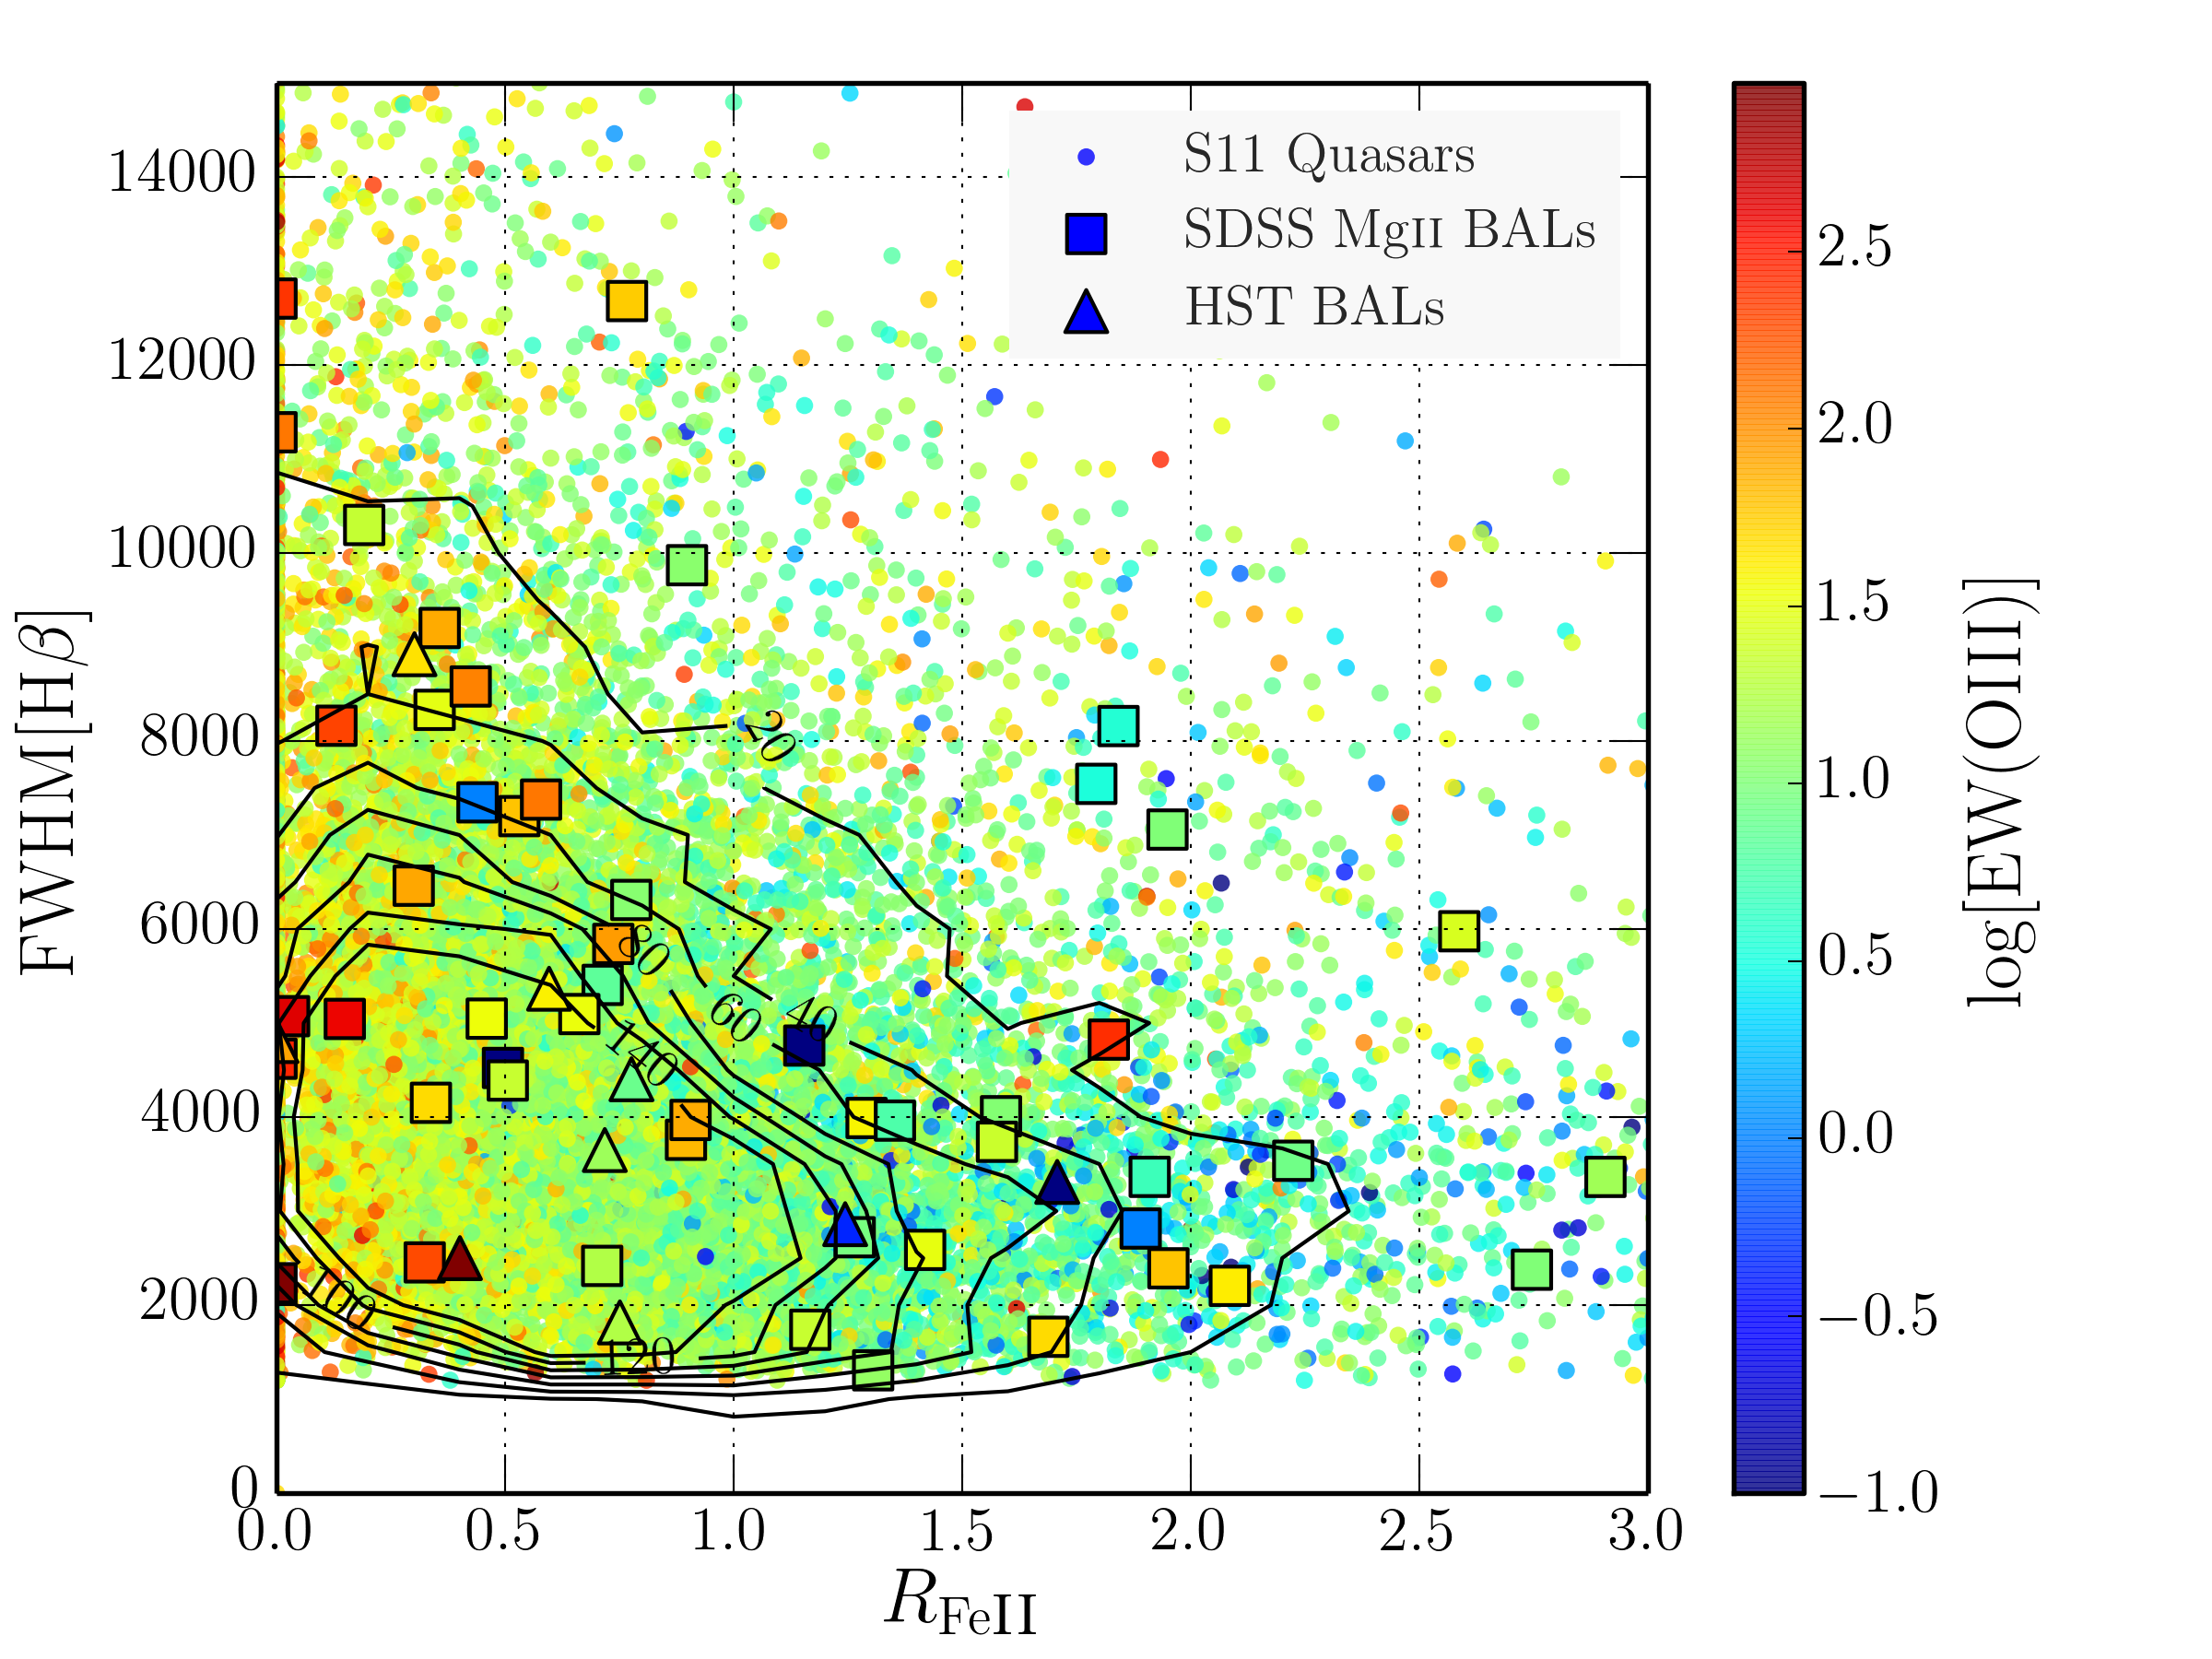
\includegraphics[width=1.0\textwidth]{figures/ewpaper/ev1.png}
\caption
[Eigenvector 1 for LoBAL and non-BAL quasars.]
{
Eigenvector 1 for BAL and non-BAL quasars. 
FWHM of the \hb\ line plotted against the relative
iron strength, $R_{{\rm Fe \textsc{ii}}}$. The colour coding
corresponds to the EW of OIII. The dots mark all quasars from
sample A, while the squares mark those with \mgii\ LoBALs. 
A few of the \mgii\ LoBALs are missing due to their lack of \fwh\ 
measurements. The shaded triangles show the approximate 
direction of the expected inclination
trend under the SH14 and R11 interpretations.
}
\label{fig:bal_ev1}
\end{figure}

\begin{figure}
\centering
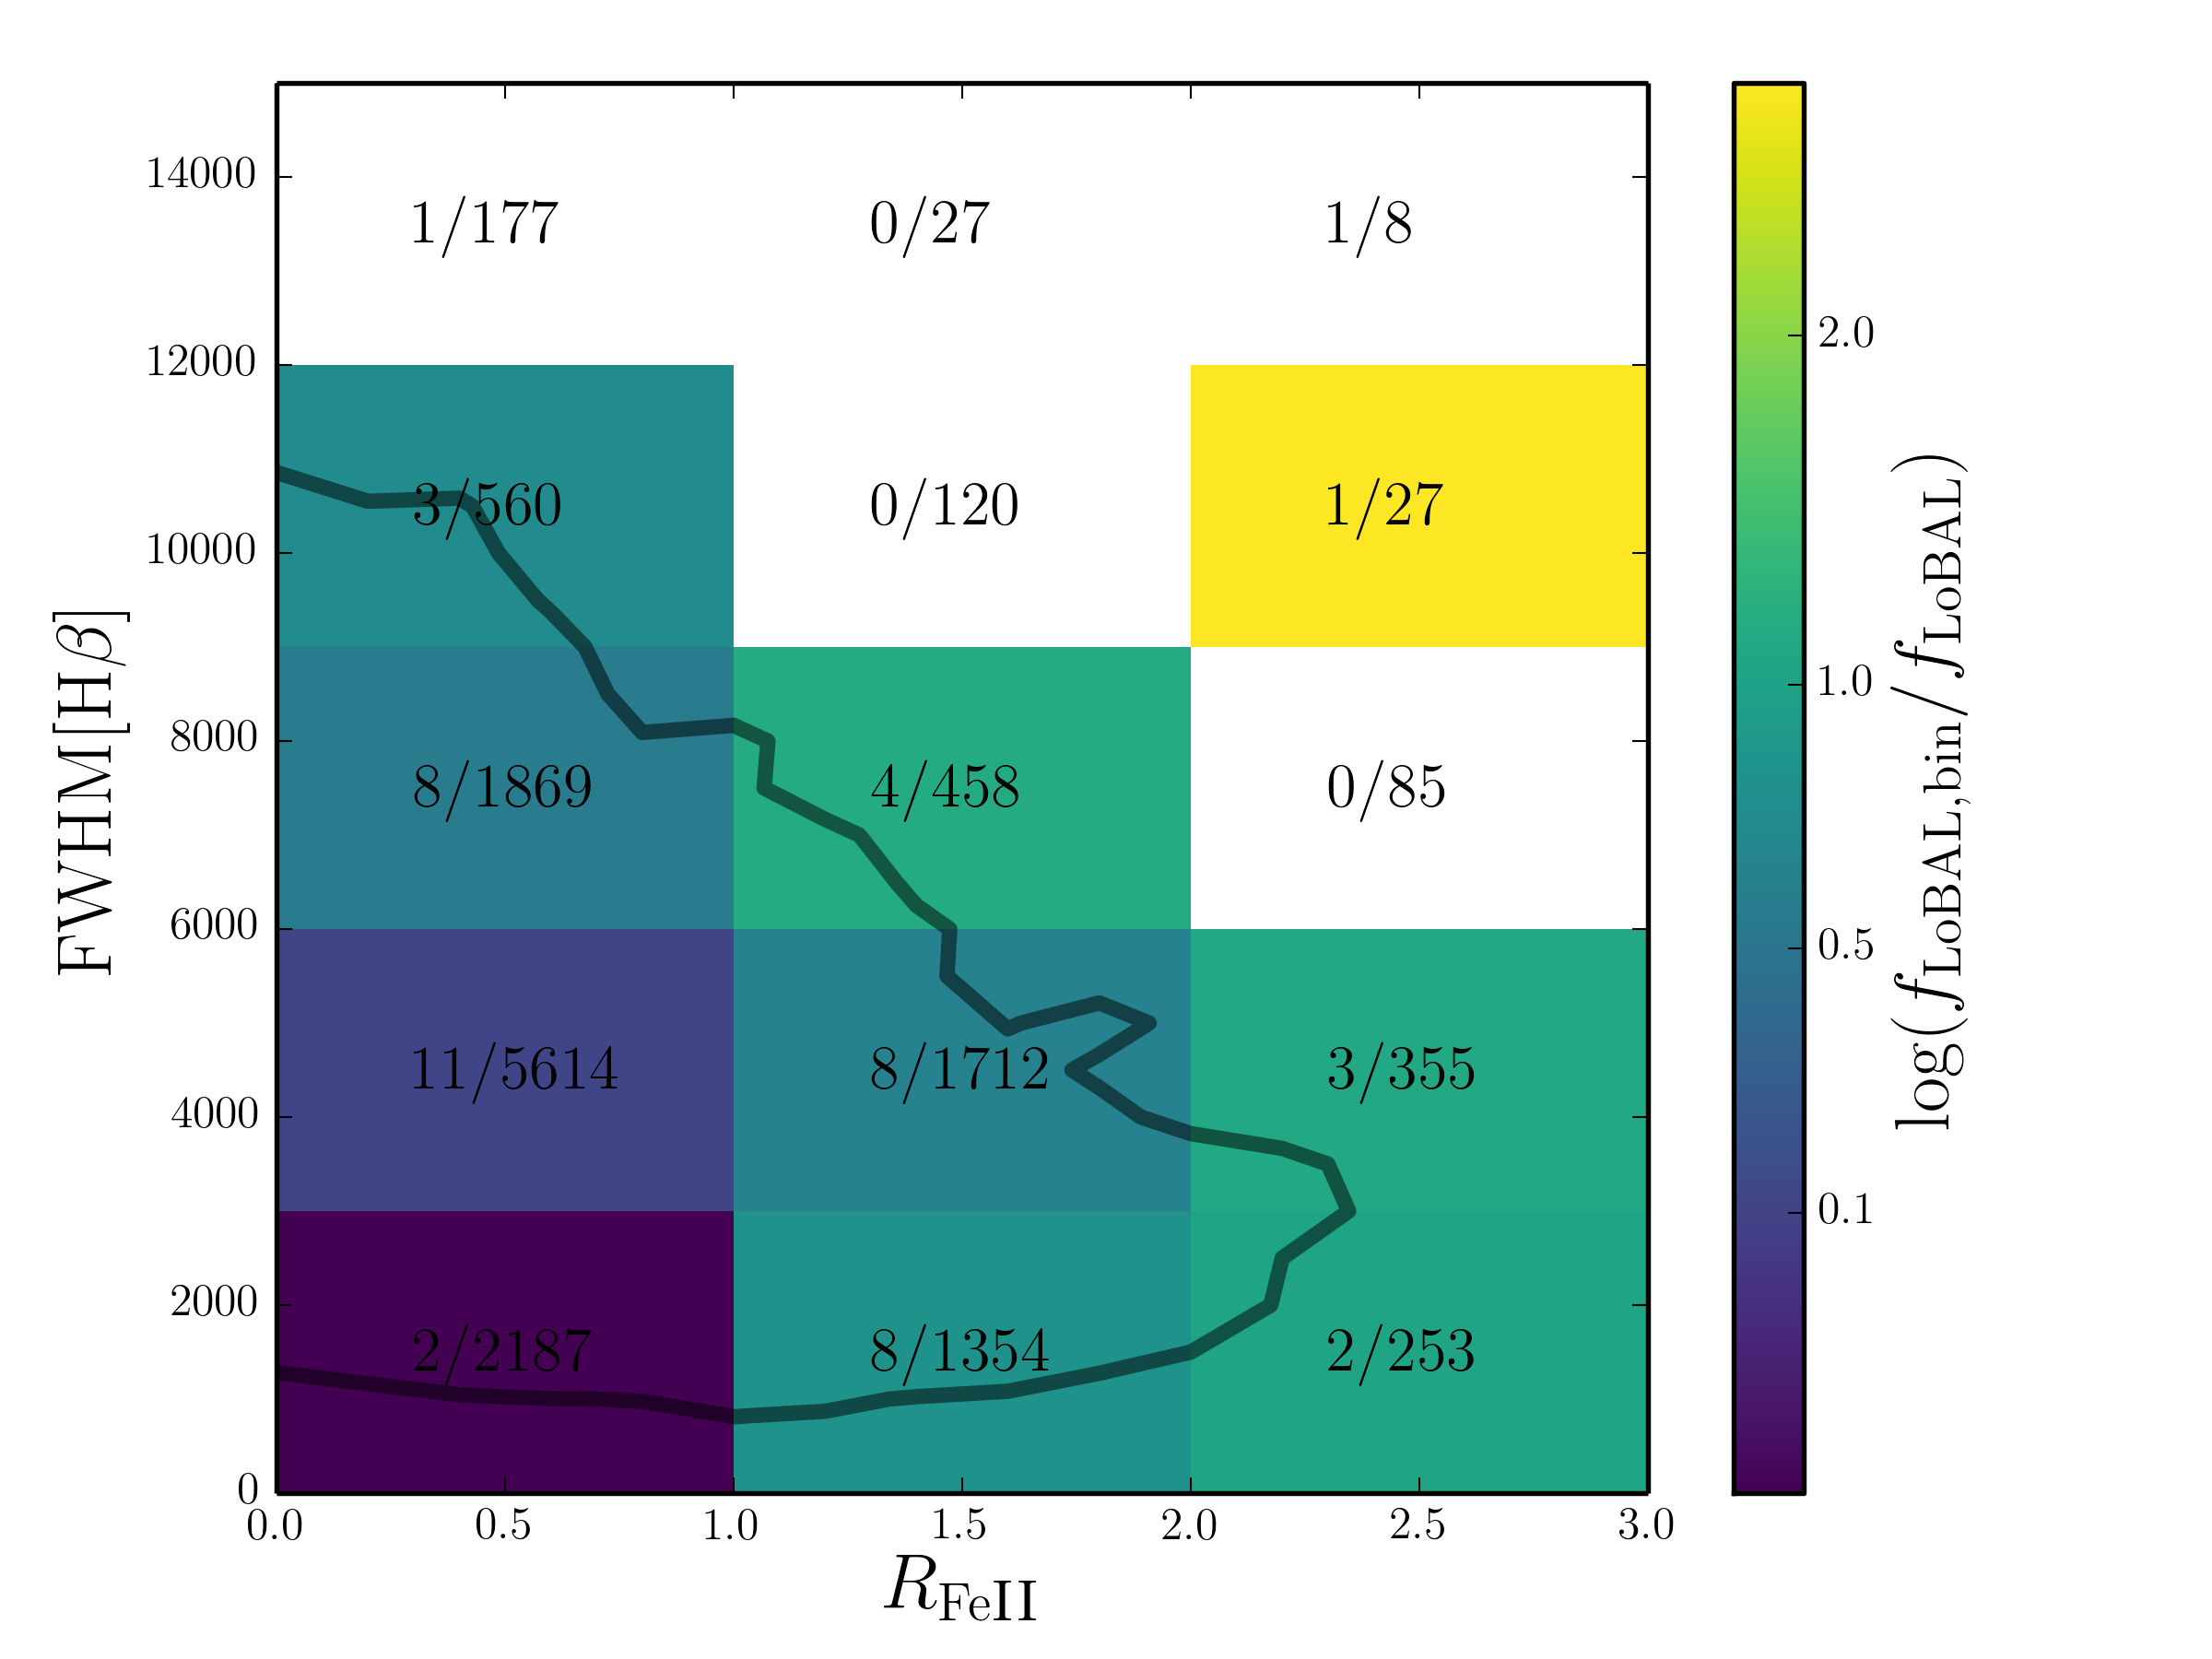
\includegraphics[width=1.0\textwidth]{figures/ewpaper/ev1_bins.png}
\caption
[LoBAL fraction compared to global LoBAL fraction in Eigenvector 1 space.]
{
LoBAL fraction compared to global LoBAL fraction in Eigenvector 1 space, in bins
of $\Delta R_{{\rm Fe \textsc{ii}}} = 1$ and $\Delta$\fwh$=3000$km~s$^{-1}$..
The contour shows the outermost contour from Fig.~\ref{fig:bal_ev1} for
reference. The text shows $N_{\mathrm{LoBAL}}/N_{\mathrm{non-BAL}}$, 
where $N_{\mathrm{LoBAL}}$ is the number of LoBALQSOs in the bin and 
$N_{\mathrm{non-BAL}}$ in the number of non-BAL quasars in the bin.
}
\label{fig:bal_ev1_bins}
\end{figure}

% \begin{figure}
% \centering
% 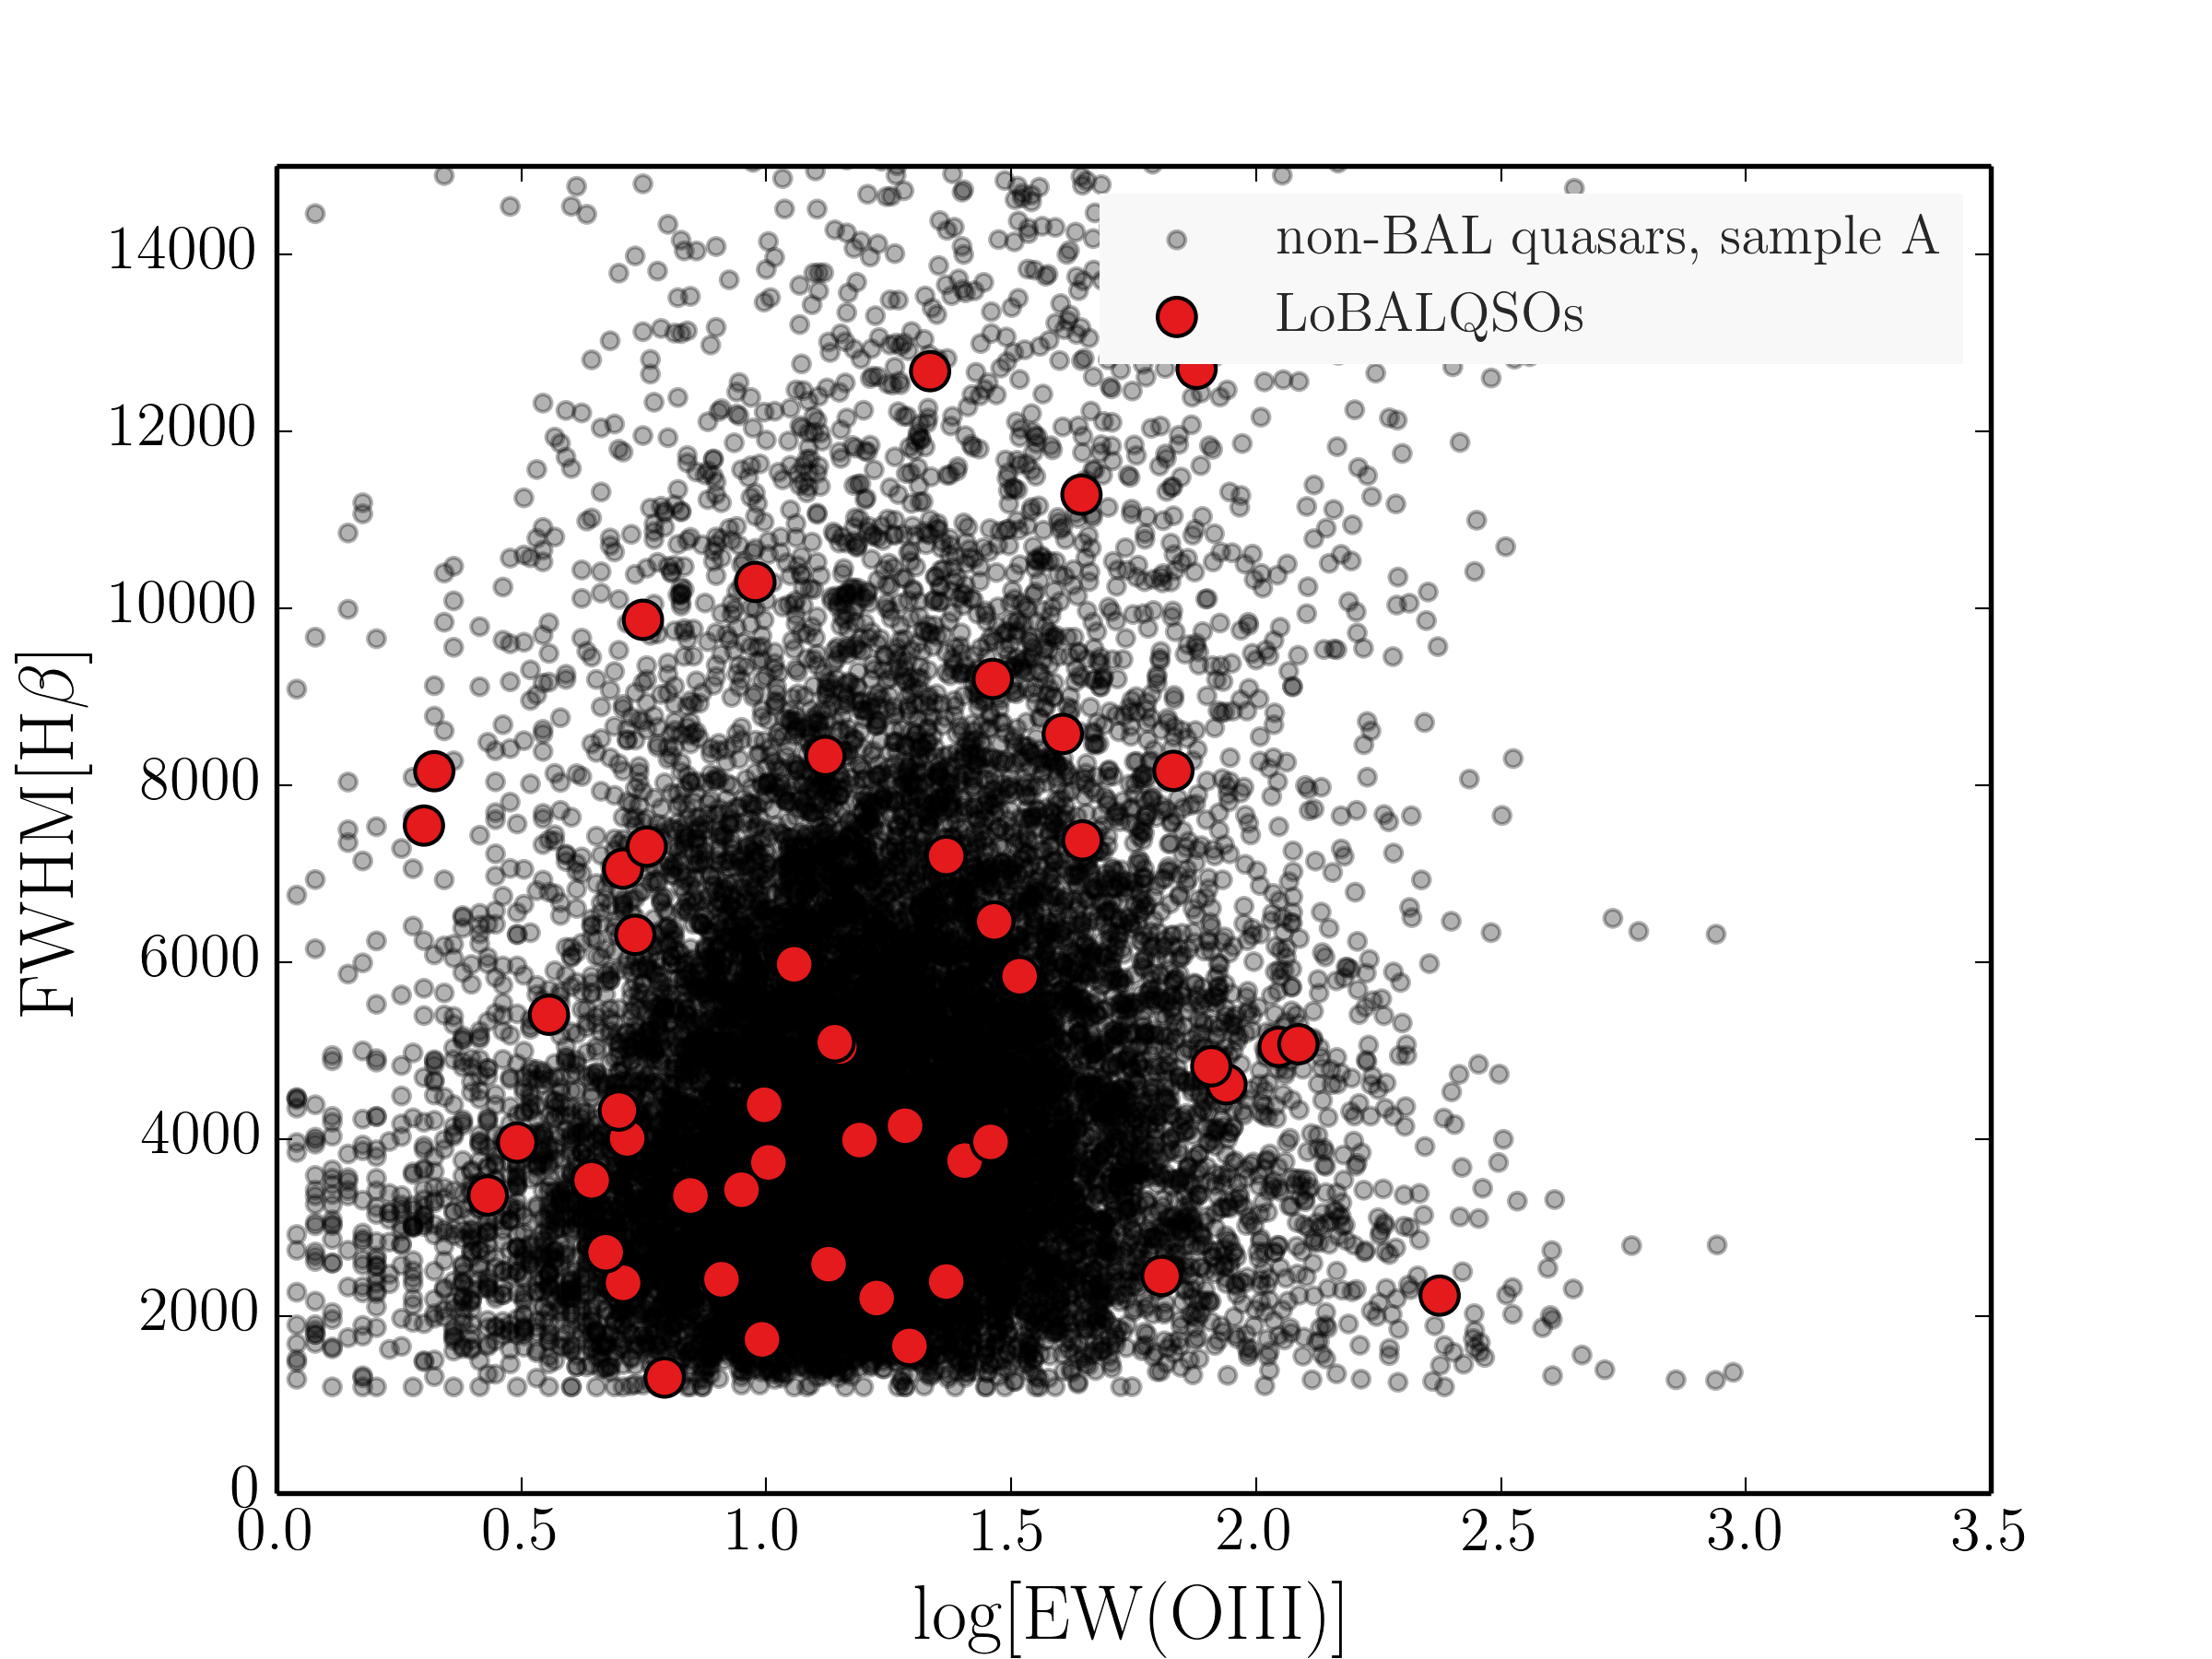
\includegraphics[width=0.8\textwidth]{figures/ewpaper/fw_v_ew.png}
% \caption
% [FWHM BLAH.]
% {
% FWHM BLAH
% }
% \label{fig:bal_ev1_bins}
% \end{figure}


% \begin{figure}
% \centering
% 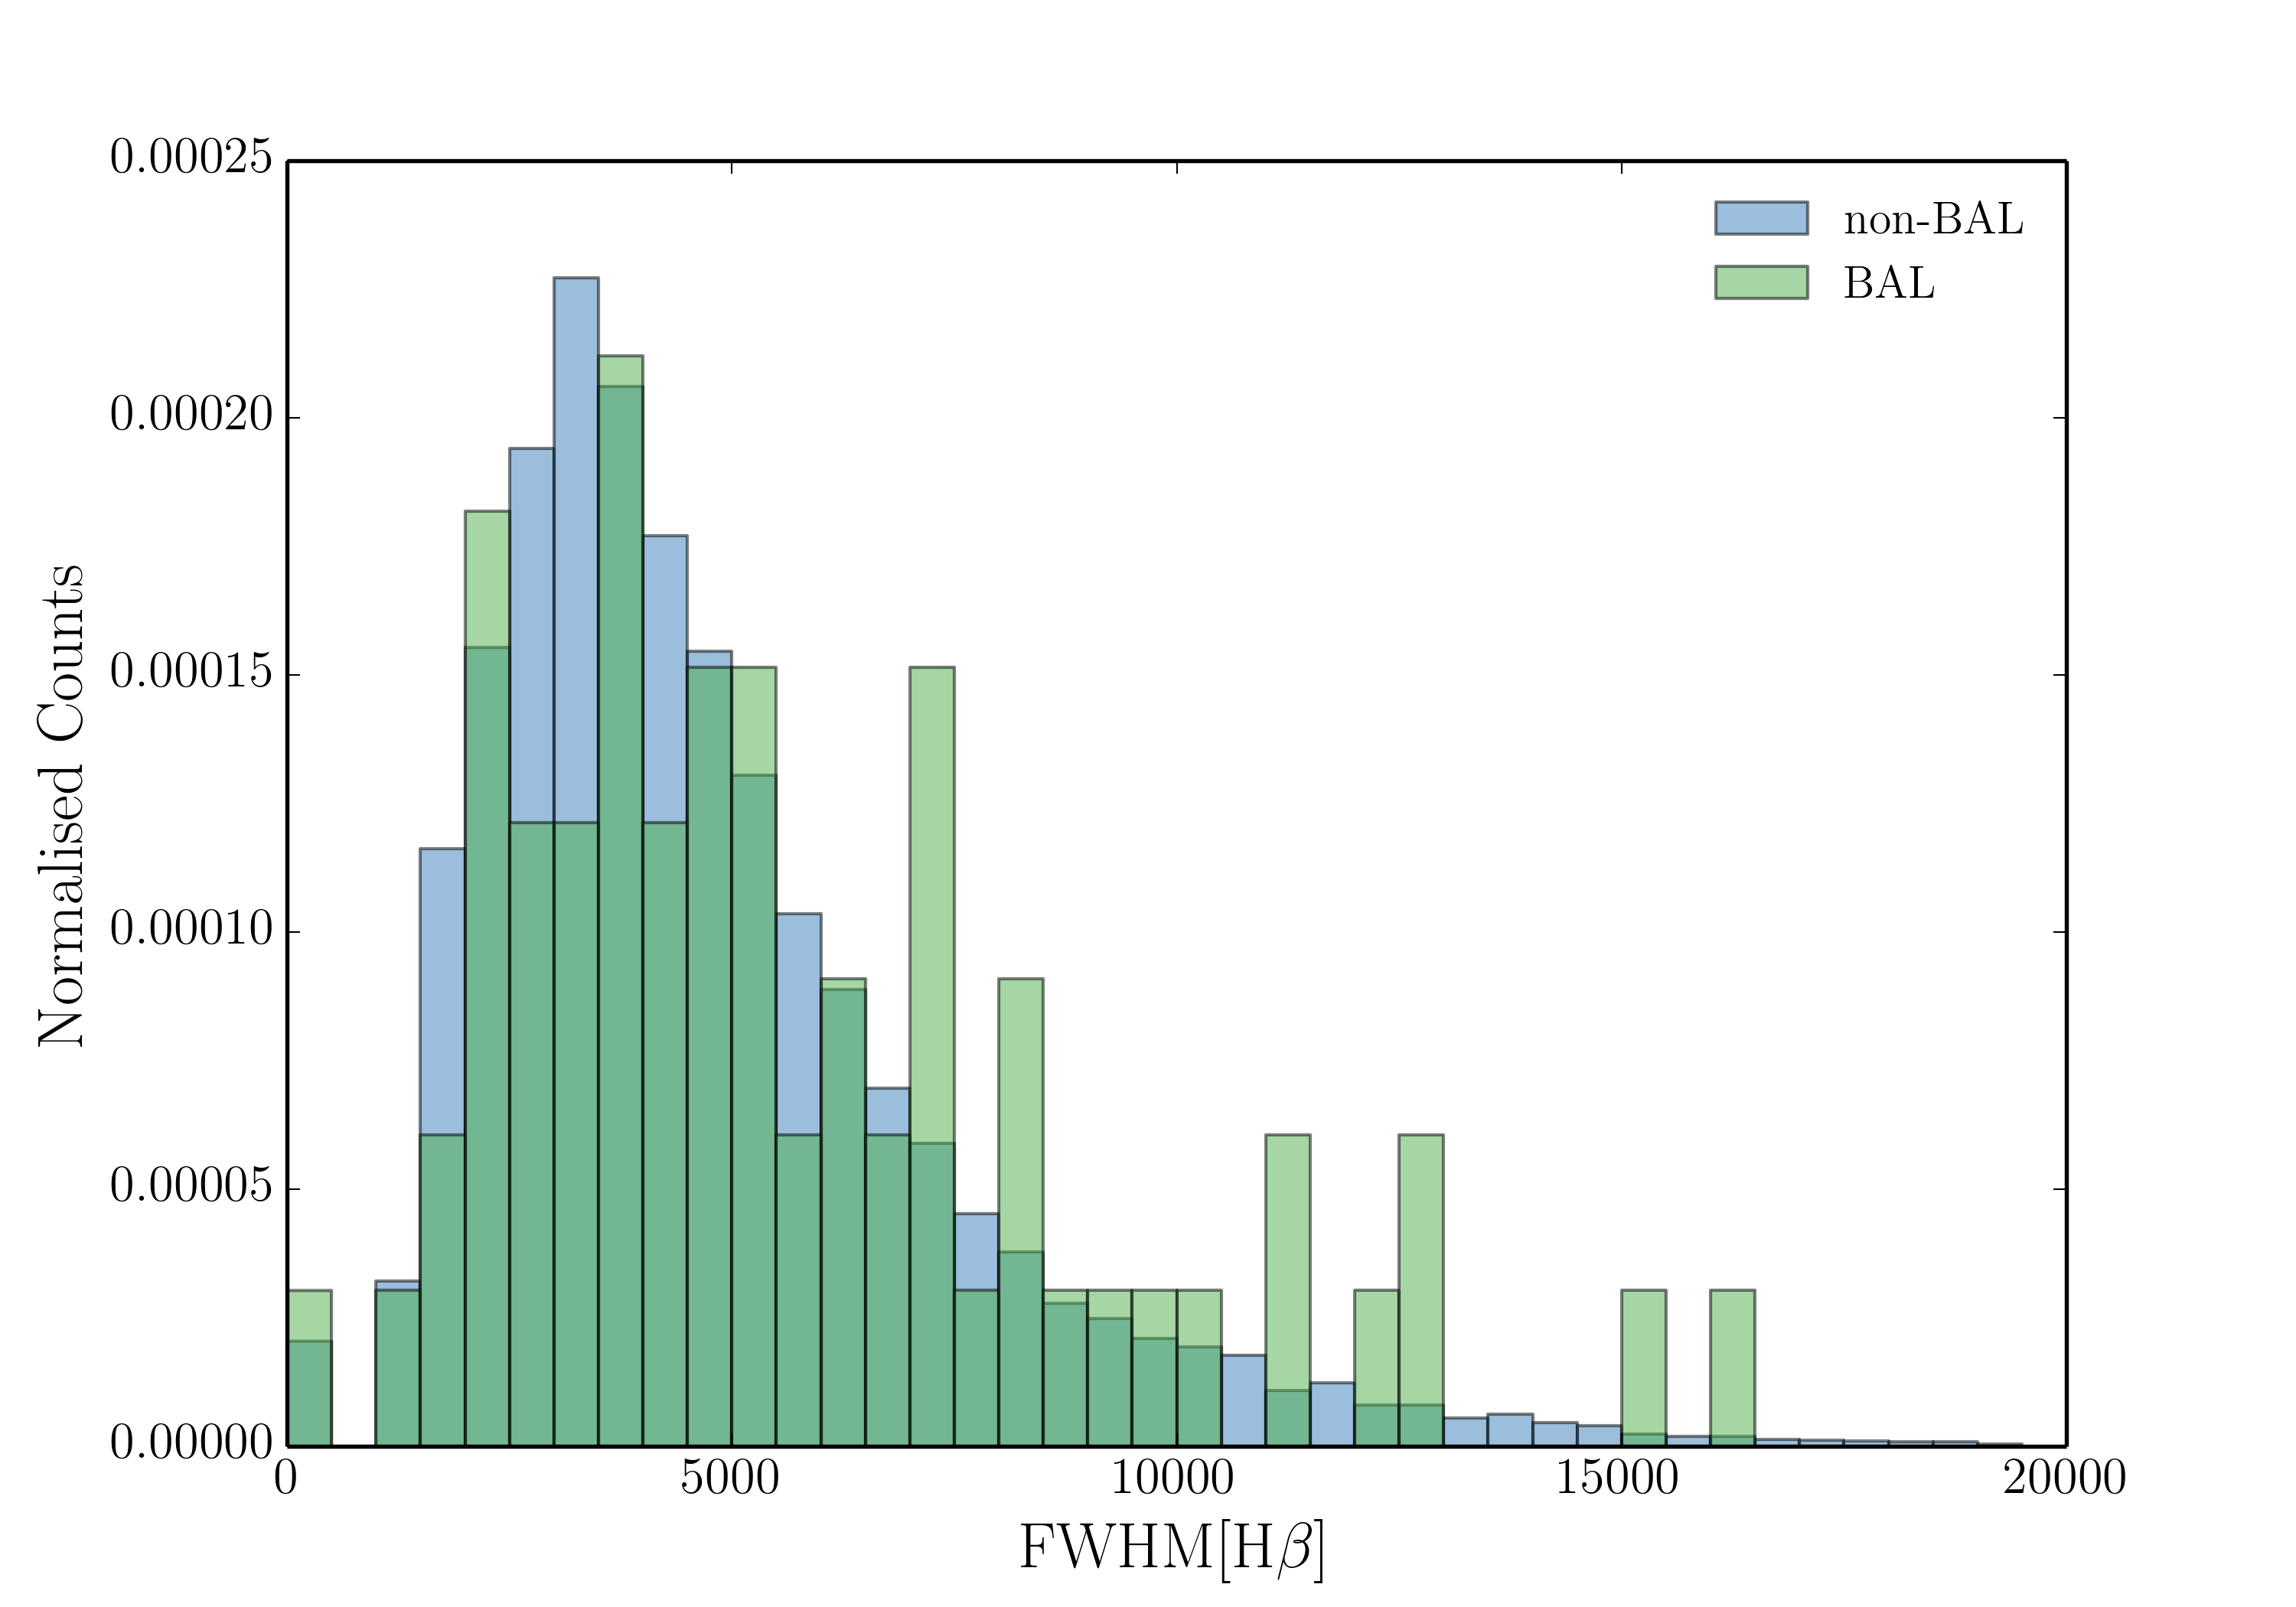
\includegraphics[width=1.0\textwidth]{figures/ewpaper/fwhm_hist.png}
% \caption
% [Distribution of \fwh\ in BAL and non-BAL quasars.]
% {
% Distribution of \fwh\ in BAL and non-BAL quasars.
% }
% \label{fig:fwhm_hb}
% \end{figure}
% \subsection{Radio Observations}
% Fig.~? shows the equivalent width distributions in radio-loud quasars, 
% split into core or lobe dominated. This designation is commonly used
% as an orientation indicator \citep{orr1982,wills1995}. 
% Although th
% In this case, we can see that 
% A full investigation of this is beyond the scope 
% {\color{blue}
% Alternative geometries and polarisation. Are there any problems with
% a more moderate viewing angle for BALs? Do we want to show a cartoon?
% Discuss modelling work. Also discuss compton-thick fraction at high mass end.
% What about PHYSICS. Can we derive lower limits on outflow angles from
% e.g. conservation of angular momentum??
% }


\subsection{Polarisation}

Spectropolarimetry of BAL quasars offers some of
the best insights into the geometries of BAL outflows and 
tends to show a few key properties. The first is enhanced 
polarisation in the BAL troughs themselves \citep{schmidt1999}. 
This is readily explained by a scattering region unobscured by the
BAL trough, with the higher polarisation percentage simply due to the
decreased direct flux. This may also explain the non-black saturation in
BAL troughs (see section~\ref{sec:balqso_angles}).

The second property 
is a continuum polarisation percentage that is around $2.4$ times greater, 
on average, than seen in the non-BAL population \citep{schmidt1999}.
A histogram of the continuum polarisation percentages of a sample of BAL quasars from 
\cite{schmidt1999} are compared to the Type I and Type II AGN 
populations from \cite{marin2014} in Fig.~\ref{fig:bal_polarisation}.
The corresponding cumulative distribution function is shown in Fig.~\ref{fig:cdf_pol}.
These show that BAL polarisation percentages seem to lie between those of type 1
and type 2 AGN. If type 1 and type 2 objects are viewed from low and high 
inclinations, respectively, as expected from unified models and suggested by
\cite{marin2014,marin2016}, this would imply  an intermediate inclination
for BALQSOs. This enhanced polarisation for BALQSOs, relative to non-BAL systems,
is also well reproduced by intermediate
inclination outflows in simple radiative transfer models \citep{marin2013}.

\begin{figure}
\centering
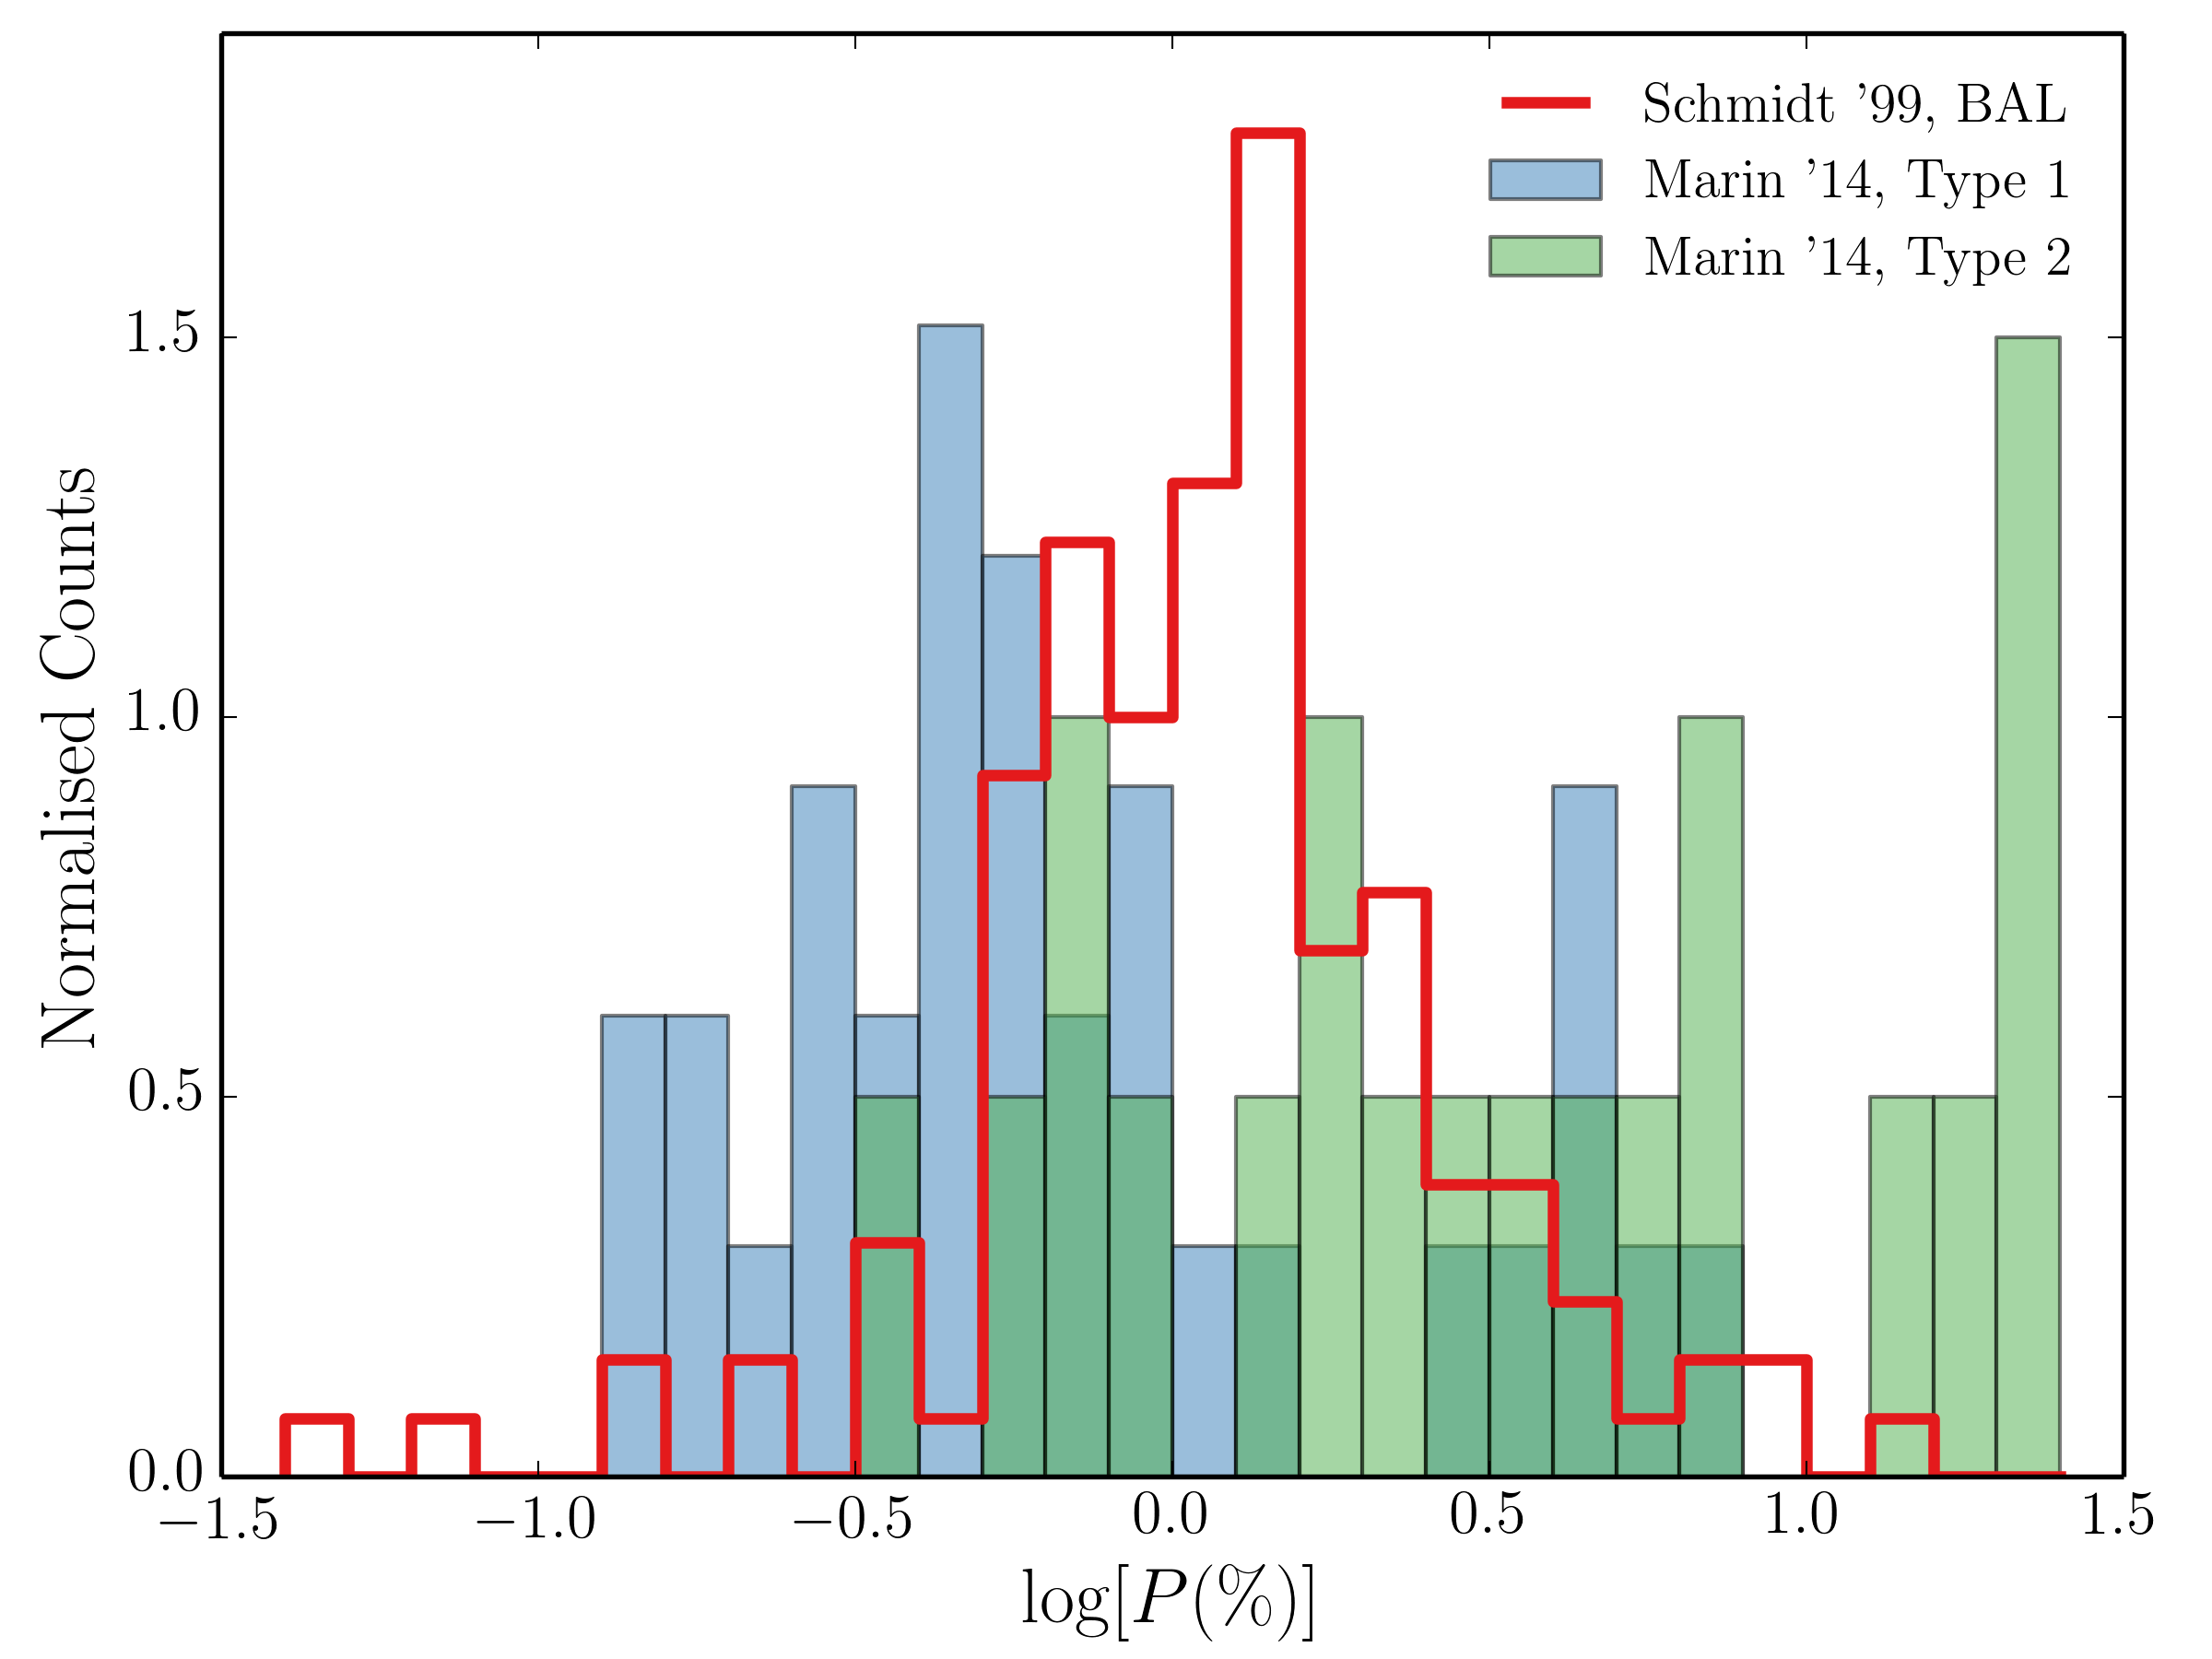
\includegraphics[width=0.8\textwidth]{figures/ewpaper/hist_p.png}
\caption
{
Histograms of polarisation percentages 
for BAL quasars from Schmidt et al. (1999) together with the 
Marin et al. (2014) AGN sample. 
}
\label{fig:bal_polarisation}
\end{figure}

\begin{figure}
\centering
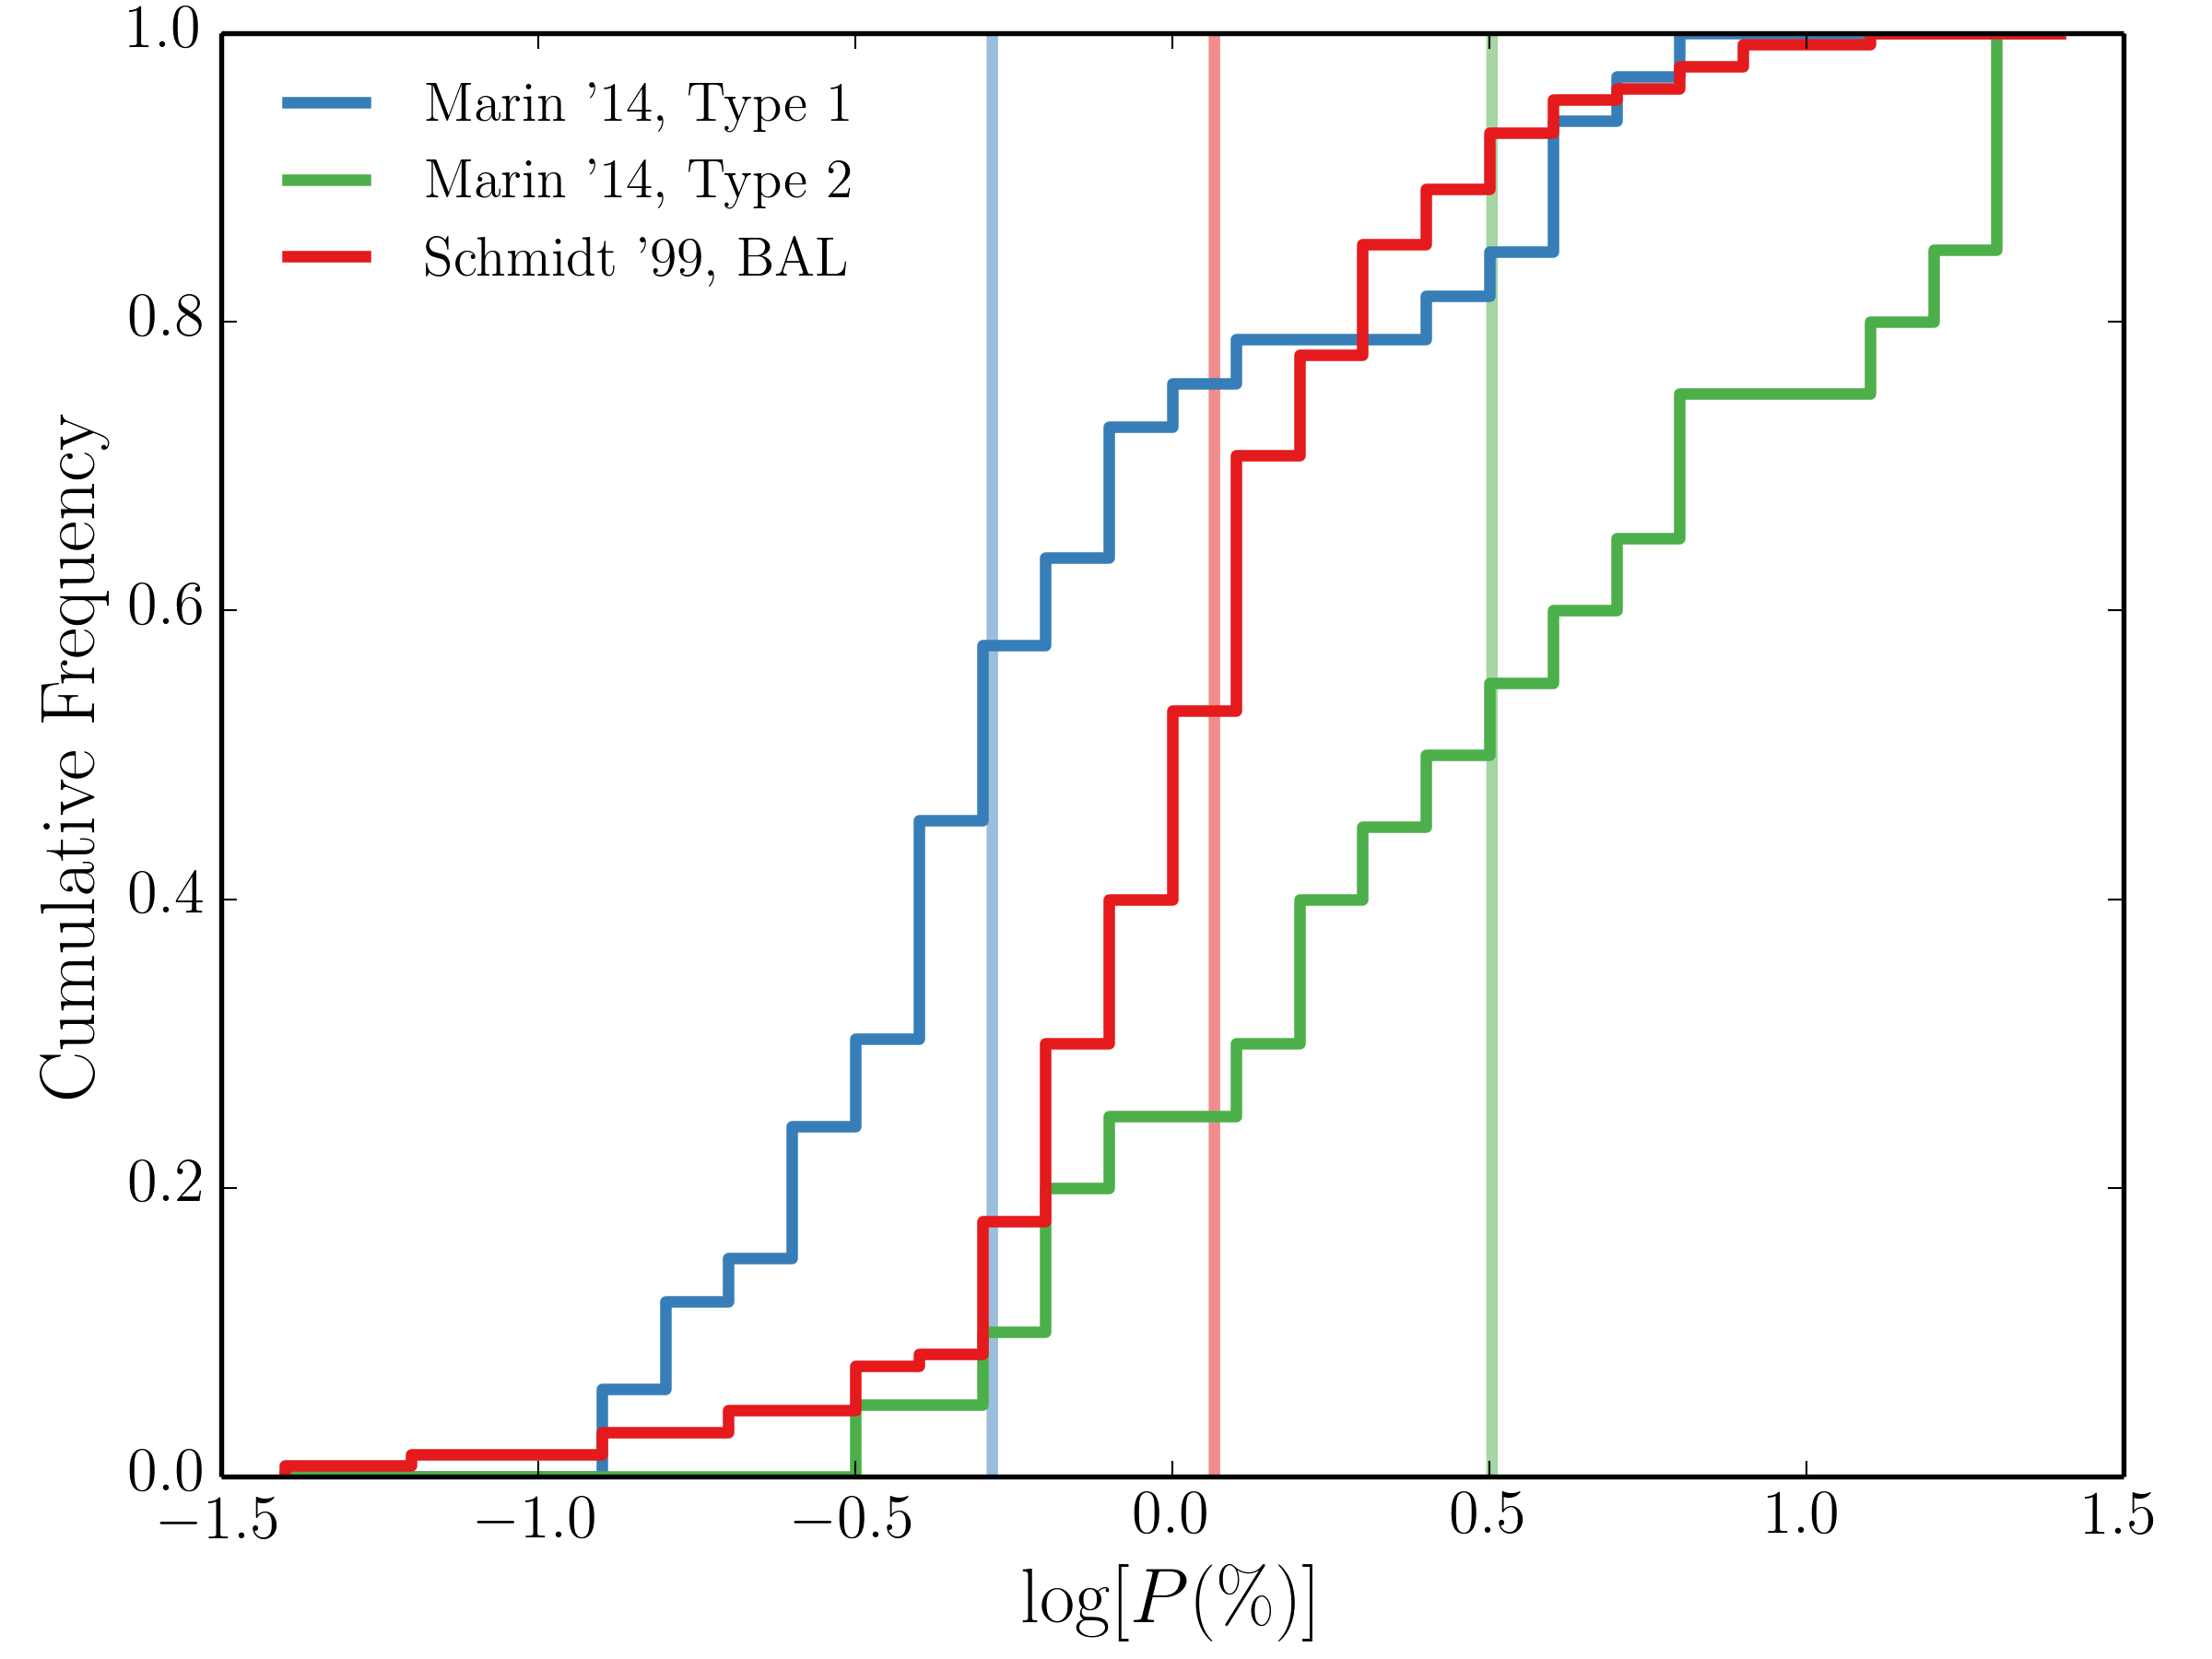
\includegraphics[width=0.8\textwidth]{figures/ewpaper/cdf_p.png}
\caption
{
Cumulative distribution functions of the histograms shown in
Fig.~\ref{fig:bal_polarisation} for BAL quasars from Schmidt et al. (1999) 
together with the Marin et al. (2014) AGN sample. The colour-coding and 
$x$-axis scale are the same as Fig.~\ref{fig:bal_polarisation}. 
The translucent vertical lines mark the median value in each sample.
}
\label{fig:cdf_pol}
\end{figure}

The third characteristic polarisation property of BALQSOs 
is a polarisation angle of $\gtrsim60^\circ$ with respect
to the radio jet axis in RL objects \citep[][and references therein]{brotherton2006}.
This suggests a higher inclination (compared to non-BAL quasars)
viewing angle for BALQSOs under the interpretation of a geometric model. Indeed,
early polarisation studies explained the observations with a polar scattering region,
viewed at an equatorial angle 
\citep[e.g.][]{goodrich1995, cohen1995,lamy2004}. Regardless of
the true geometry, the reason for the difference must be understood.
I would suggest that polarisation predictions are made from wind
models such as the one I presented in chapter 5, using a similar
approach to \cite{marin2013}, but considering BALs in more detail. 
Overall, however, polarisation measurements seem to imply that BALQSOs are viewed
from higher inclinations if geometric unification models are correct and are 
in slight tension with the idea that BAL quasars are viewed from the same range
of angles as non-BAL quasars.

\subsection{The Effect of Obscuration}
\label{sec:obscure}

\citet[][hereafter C11]{caccianiga2011} showed that the distribution of \ewo\
can also be well fitted by an obscuration model. They modelled the 
\ewo\ distribution using an absorption model based on column densities
obtained from the {\sl XMM Newton} Bright Serendipitous Source (XBS)
sample. They use a sample size of 169 objects, and find that AGN with 
column densities of $N_H\gtrsim10^{22}$~cm$^{-2}$ can explain the high
EW powerlaw tail. 

The column density measurements for BAL quasars suggest that obscuration 
cannot explain the distribution of \ewo\ in quasars. 
As briefly discussed in chapter 5, BALs generally show
strong X-ray absorption with column densities of $N_H\gtrsim10^{23}$~cm$^{-2}$
\citep{green1996,mathur2000,green2001,grupemathur2003}. \cite{gallagher1999}
found all BAL quasars in a sample of 7 had $N_H>10^{22}$~cm$^{-2}$, placing
them firmly in the EW tail according to the C11 model. This is broadly
consistent with the mean value of $3.5\times10^{22}$~cm$^{-2}$ from
\cite{morabito2013}, and would imply that BALQSOs should have significantly
higher EWs if obscuration governs the \ewo\ distribution.
Of course, only LoBAL quasars had \ewo\ measurements 
in the sample used here -- this actually strengthens the conclusion, as low ionization 
BALQSOs show even higher column densities, approaching Compton-thick values 
\citep{morabito2011}. This argument regardless of the outflow geometry adopted,
so I suggest that the obscured model of C11 is ruled out on this basis.


\subsection{Line Anisotropy}
\label{sec:line_aniso}

Optically thin lines are isotropic -- the {\em local}
escape probabilities in each direction are equal due to the 
low optical depth. When lines are optically thick, the situation is more
complex, as local velocity gradients then determine the line 
anisotropy. Indeed, Keplerian velocity shear has been shown to modify the
shape of disc-formed emission lines \citep{hornemarsh1986}, and an additional
radial shear from a wind can cause double-peaked lines
to become single-peaked \citep{MC96,MC97,flohic2012}.

R11 suggested that the broad emission lines trace the disc
emission in terms of their anisotropy. 
If this was the case, we would not expect a difference in the BAL and non-BAL
quasar EW distributions. However, an emission line would only be purely 
foreshortened if emitted by a disc with zero velocity shear. 
If the lines came from a region subject to
Keplerian velocity shear then the surface brightness of an optically thick 
line is \citep{hornemarsh1986}
\begin{equation}
J_{\mathrm{thick}}(\theta) \approx \cos \theta~S_L~\Delta \nu~\sqrt{8 \ln \tau_0} \ ,
\end{equation}
where $S_L$ is the line source function (assumed constant) and
$\tau_0$ is the line centre optical depth, given by
\begin{equation}
\tau_0 = \frac{{\cal W}}{\sqrt{2}\pi \Delta \nu \cos \theta}.
\end{equation}
The parameter ${{\cal W}}$ is given by
\begin{equation}
{{\cal W}} = \frac{\pi e^2}{m_e c}f N^\prime,
\end{equation}
where $f$ is the oscillator strength and $N^\prime$ is the number
density integrated along the vertical height of the disc. The linewidth
$\Delta \nu$ is enhanced from the thermal line width by the velocity shear, such
that
\begin{equation}
\Delta \nu = \Delta \nu_{th} \left[1 + 
\left(\frac{3}{4}\frac{v_{k}}{v_{th}}\frac{H}{R}\right)^2
Q(\theta, \phi)
\right]^{1/2},
\end{equation}
where I have defined
\begin{equation}
Q(\theta, \phi) =
\sin^2 \theta \tan^2 \theta \sin^2 2 \phi.
\end{equation}
Here, $\phi$ is the azimuthal angle in the disc, $\nu_{th}$ and $v_{th}$ are the 
thermal line widths in frequency and velocity units respectively, 
$H$ is the scale height of the disc at radius $R$, and $v_k$ is the
Keplerian velocity. The outcome of the \cite{hornemarsh1986} analysis is that optically thick lines 
formed in a Keplerian disc are strongly anisotropic, but they do not follow a simple 
$\cos \theta$ distribution. Instead, the line anisotropy is
a function of the velocity shear in the disc, the atomic physics of
the line in question, the location of the line formation region 
and the vertical disc structure. 

To examine the form of this line anisotropy, 
we can now define the angular emissivity function for a line, $\epsilon_{\mathrm{line}}(\theta)$.
In the optically thick case with no additional velocity shear, 
$\epsilon_{0,\mathrm{line}}(\theta) = \cos \theta$.
In the presence of Keplerian velocity shear, and neglecting the weak $\sqrt{8 \ln \tau_0}$ term, 
we can write
\begin{equation}
\epsilon_{k, \mathrm{line}}(\theta, \phi) = \cos \theta \left[1 + 
\left(\frac{3}{4}\frac{v_{k}}{v_{th}}\frac{H}{R}\right)^2
Q(\theta, \phi)
\right]^{1/2}.
\end{equation}
This quantity is compared to $\cos \theta$ in Fig.~\ref{fig:line_aniso1} 
as a function of for a few values of $\phi$, 
using typical quasar parameters of $v_k=10,000~\mathrm{km~s^{-1}}$ and 
$v_{th}=10~\mathrm{km~s^{-1}}$, and assuming $H/R=0.01$. I also show the 
azimuthally-averaged function, $\bar{\epsilon}_{k,\mathrm{line}}$, 
which determines the integrated emergent flux as a function of $\theta$.
Fig.~\ref{fig:line_aniso2} also shows $\bar{\epsilon}_{k,\mathrm{line}}$ 
for a few different model values of $v_k, v_{th}$
and $H/R$; the models are defined in table~\ref{tab:line_mods}.

\begin{figure}
\centering
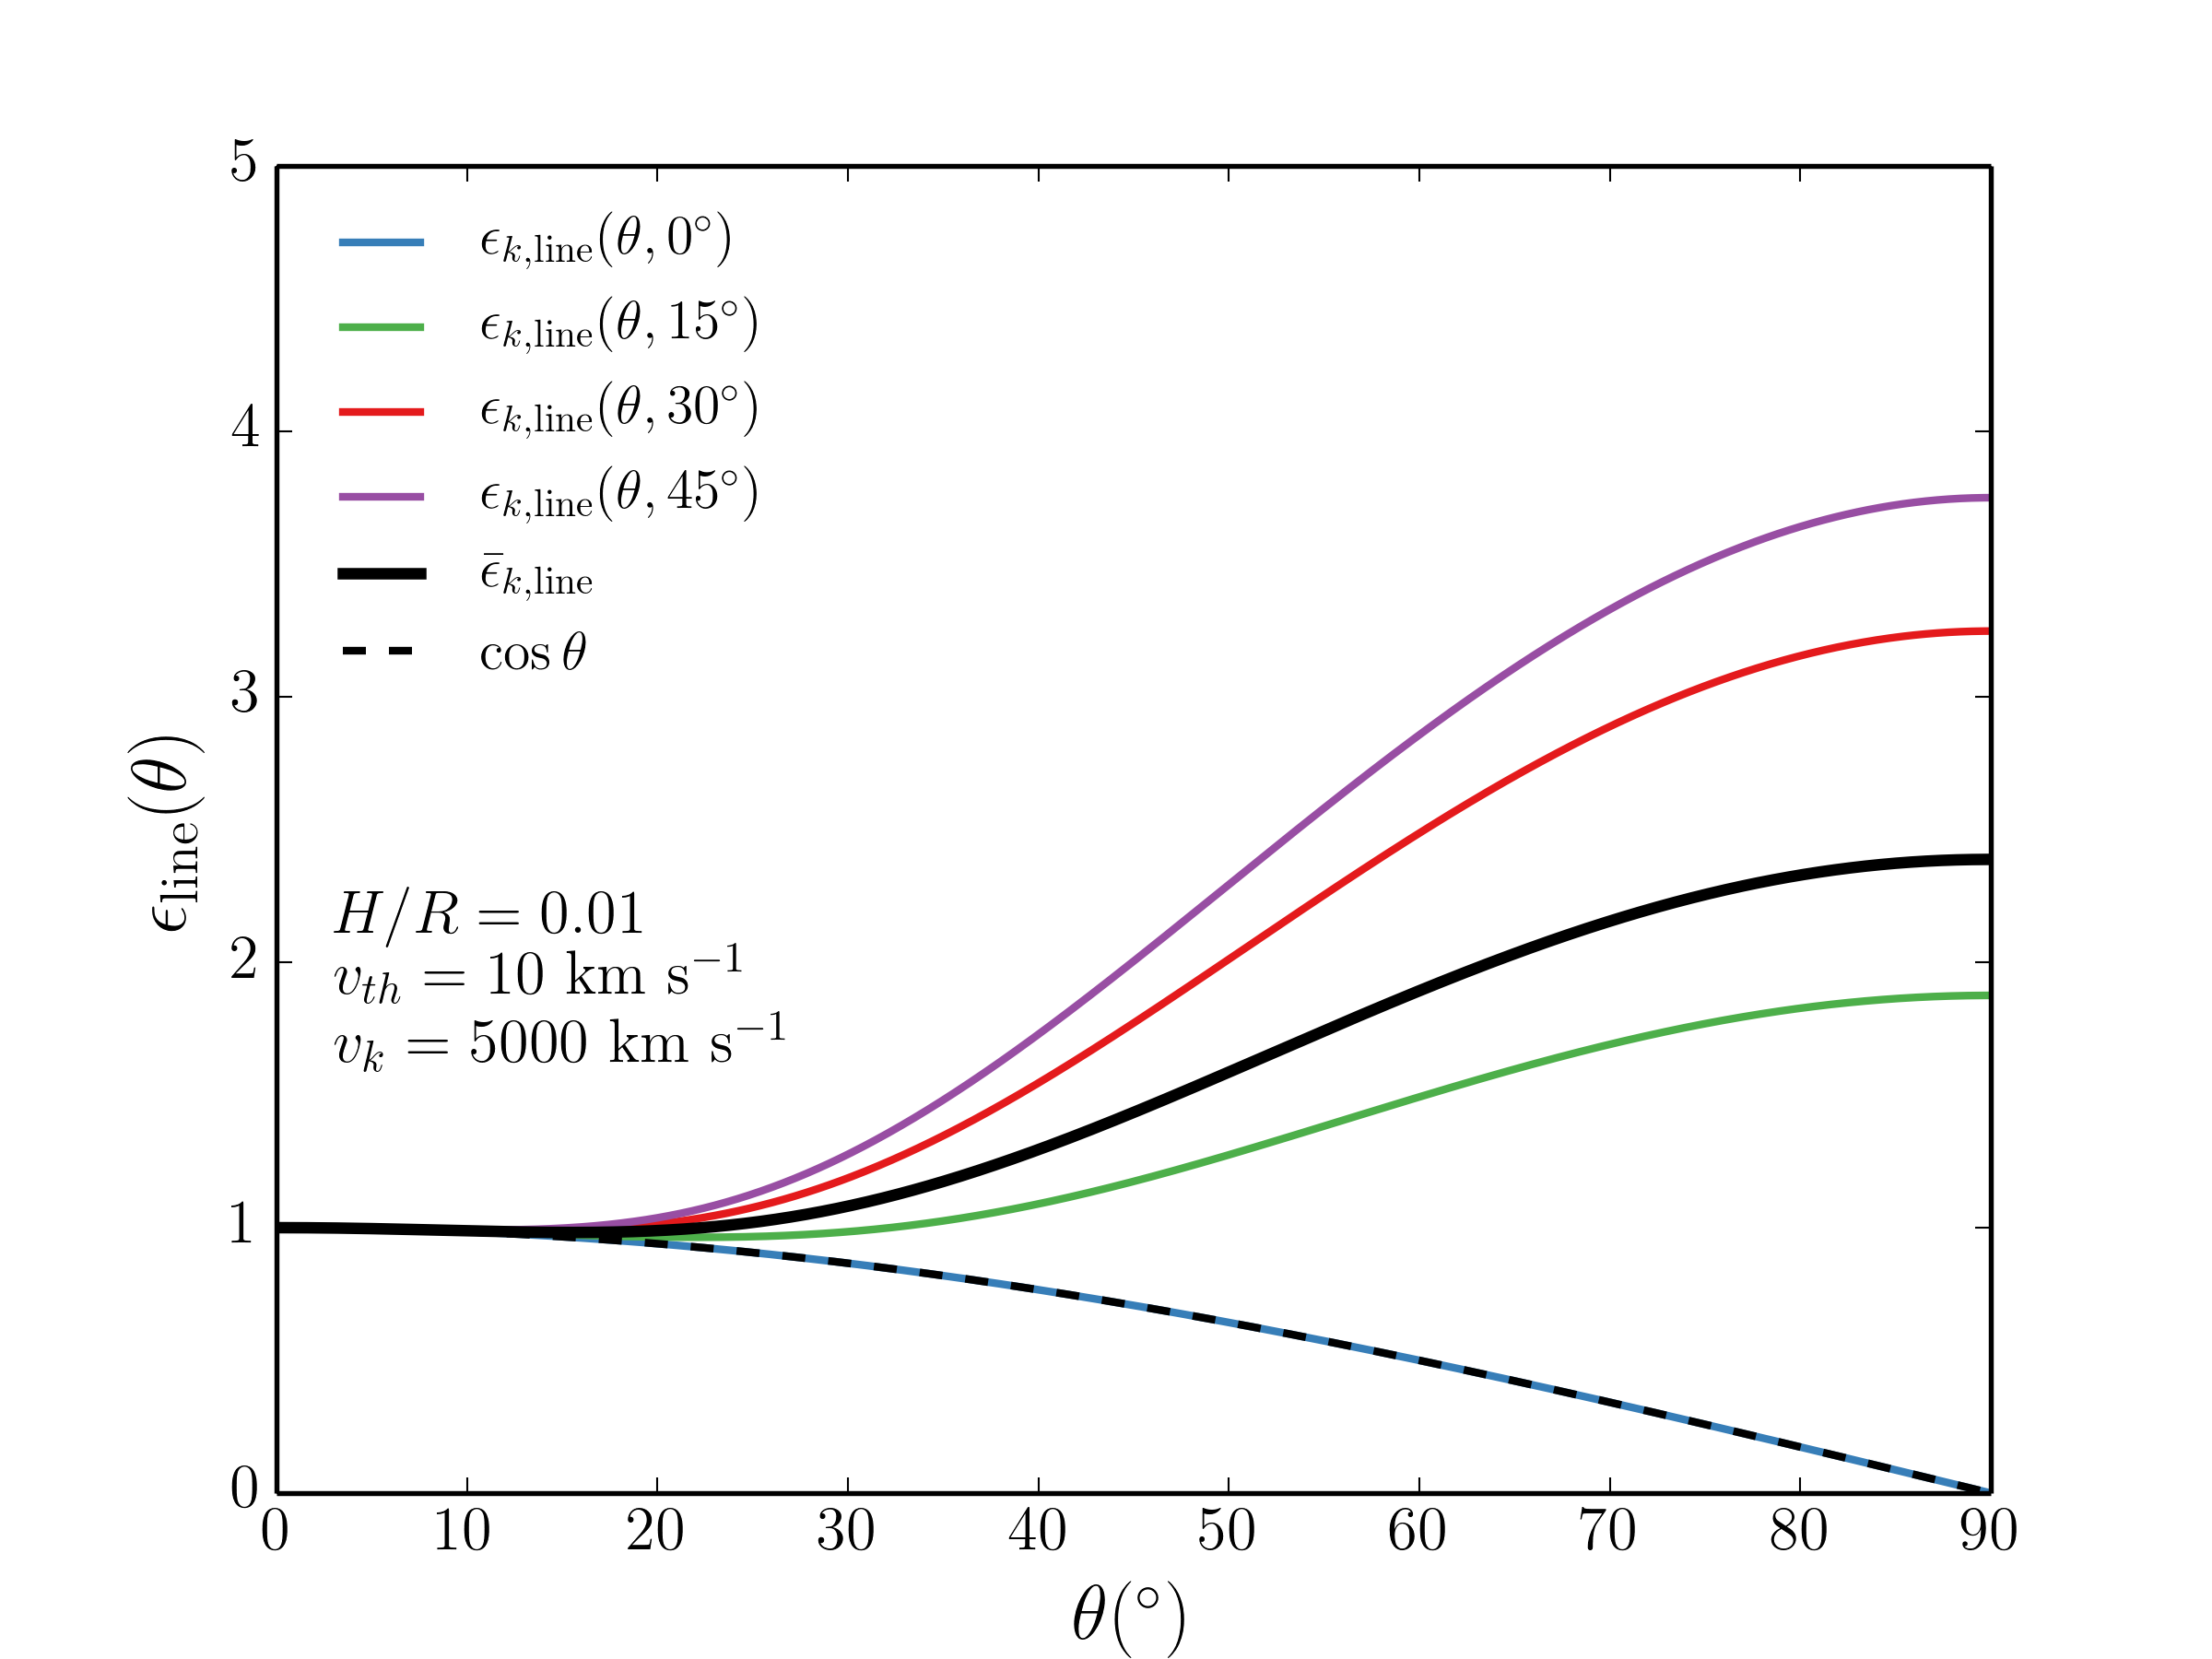
\includegraphics[width=1.0\textwidth]{figures/ewpaper/line_azi.png}
\caption
{
LINE BLAH
}
\label{fig:line_aniso1}
\end{figure}


\begin{figure}
\centering
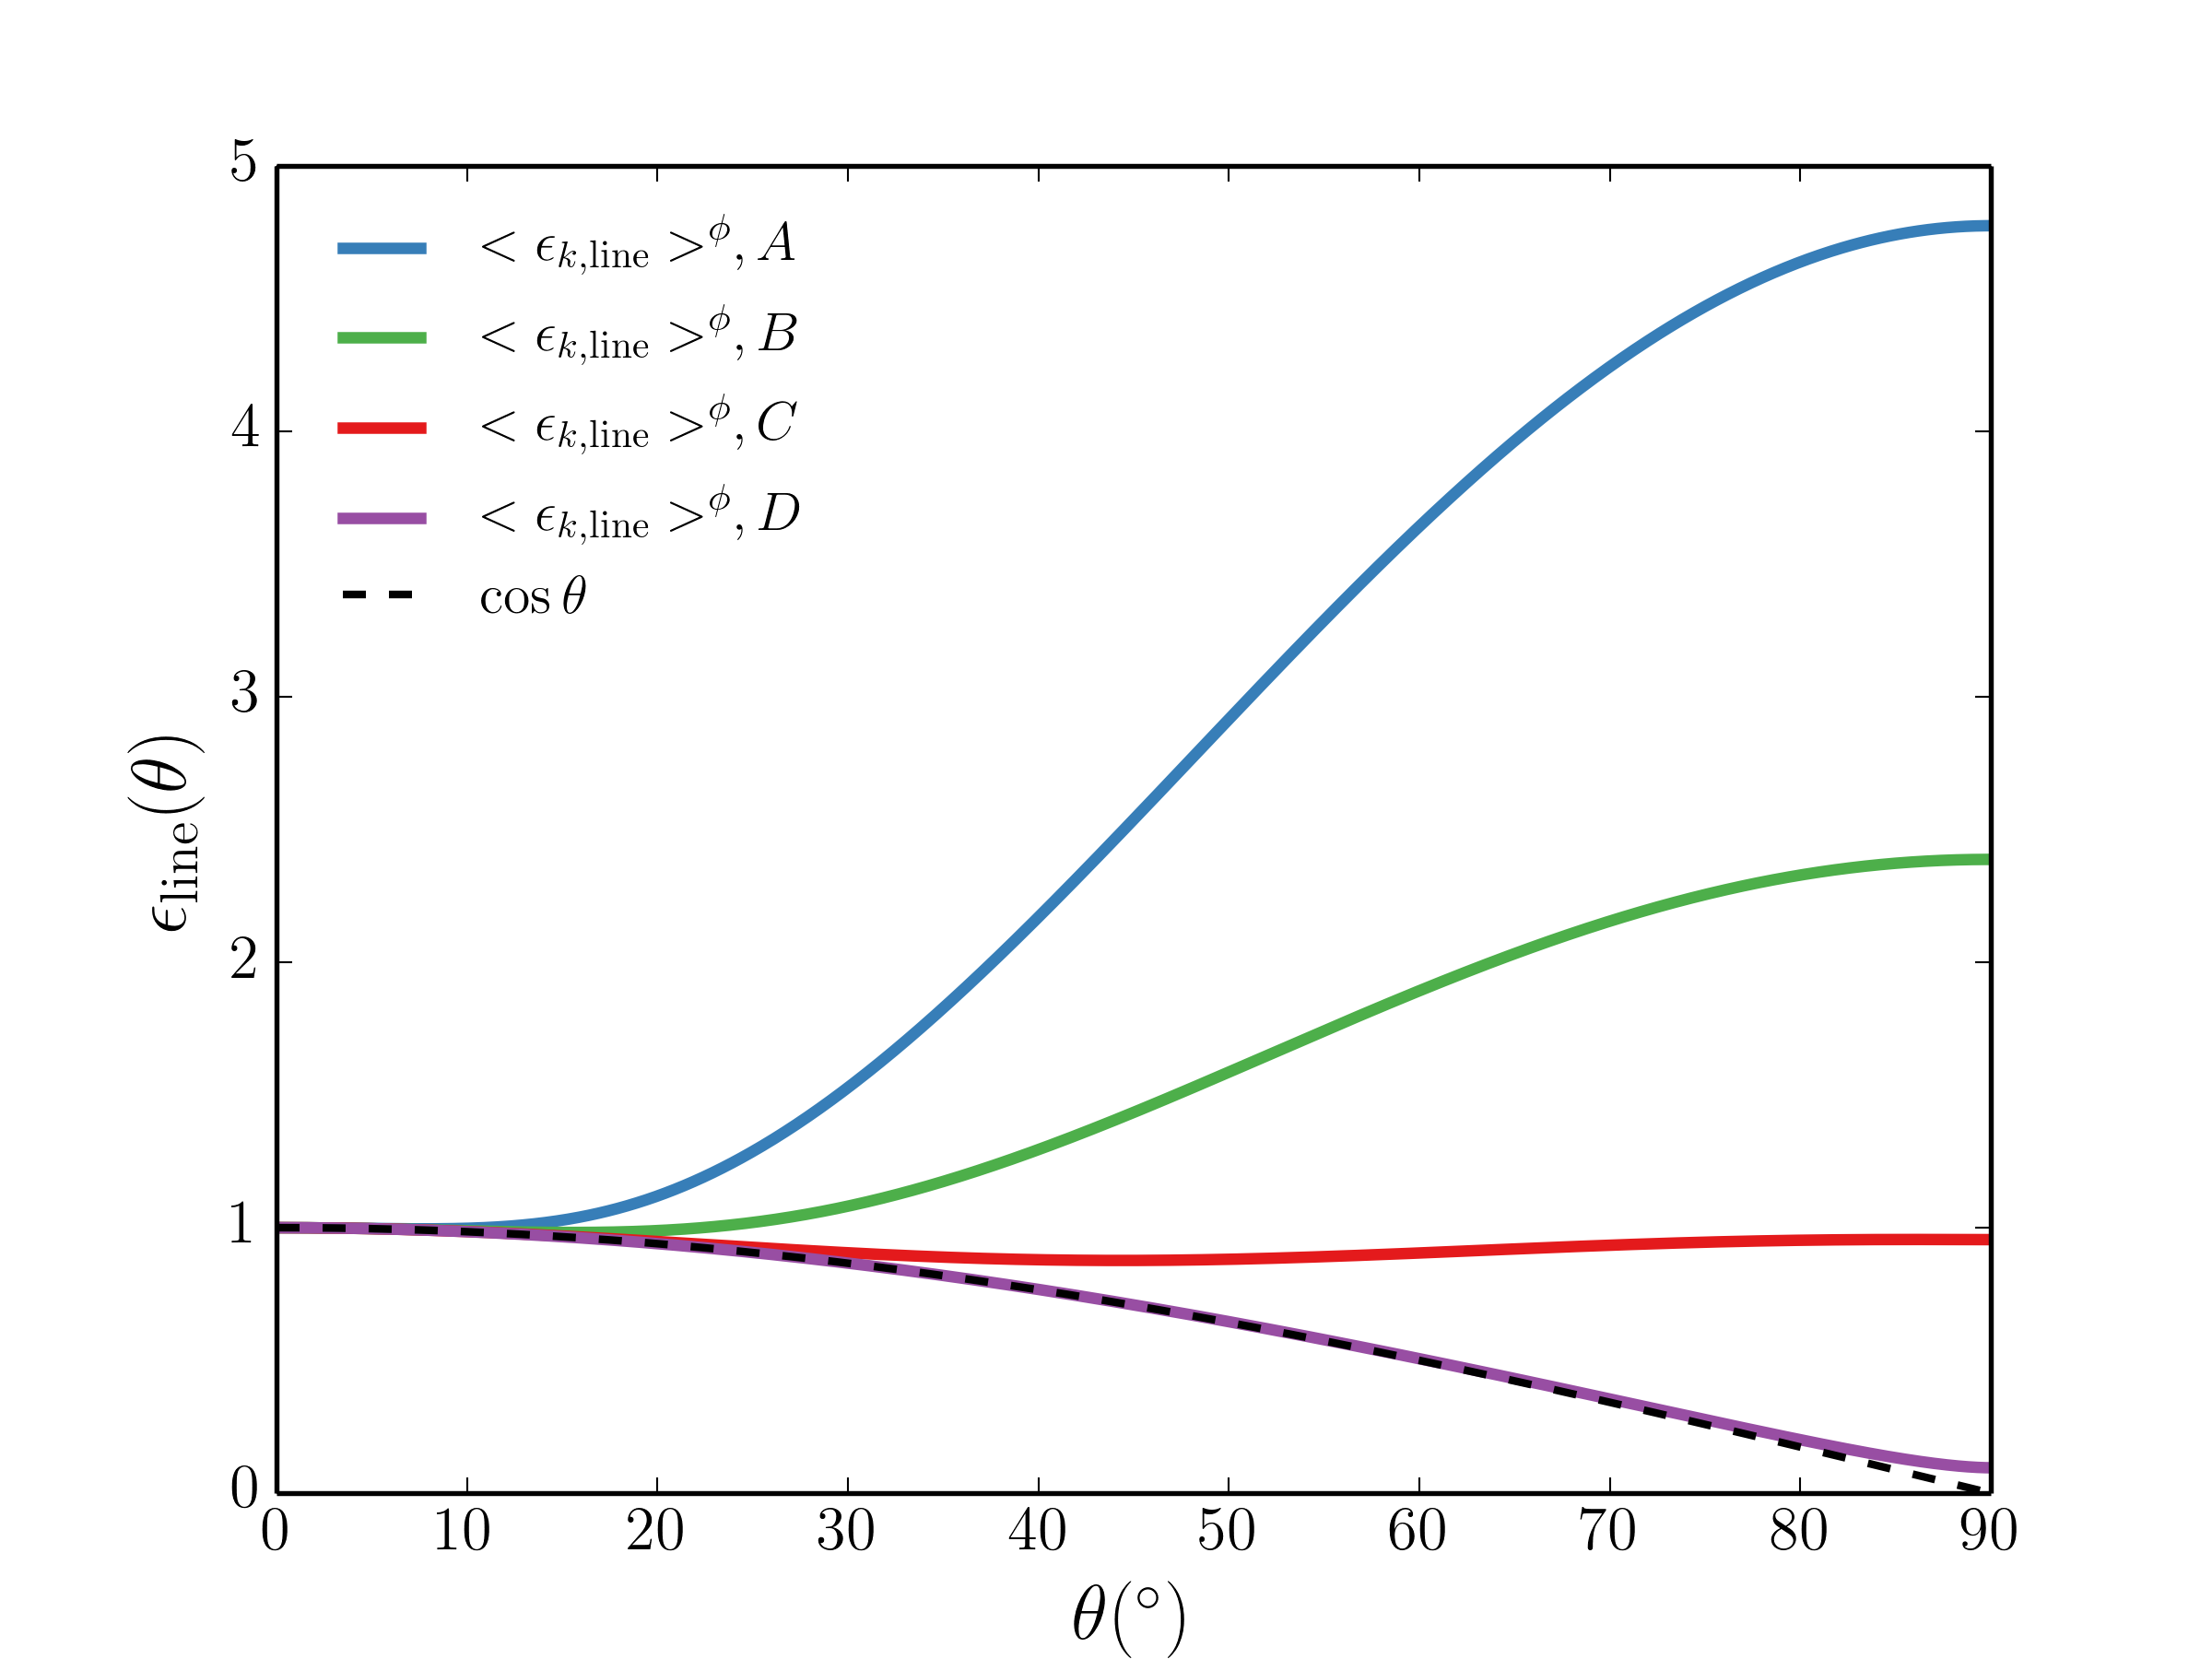
\includegraphics[width=1.0\textwidth]{figures/ewpaper/line_emiss.png}
\caption
{
LINE BLAH
}
\label{fig:line_aniso2}
\end{figure}

\begin{table}
\centering
\begin{tabular}{p{1cm}p{2cm}p{2cm}p{2cm}p{2cm}}
\hline
Model & $H/R$ & $v_k (\mathrm{km~s^{-1}})$ & $v_{th} (\mathrm{km~s^{-1}})$ \\
\hline \hline 
A & $0.01$ & $10,000$ & $10$ \\
B & $0.01$ & $5,000$ & $10$ \\
C & $0.01$ & $5,000$ & $25$ \\
D & $0.001$ & $5,000$ & $25$ \\
\hline 
\end{tabular}
\caption{
The values of the Keplerian velocity, $v_k$, thermal velocity, $v_{th}$,
and ratio of disc scale height to radius, $H/R$, for four models. These values
are used as inputs to calculate $\bar{\epsilon}_{k,\mathrm{line}}$ as shown in 
Fig.~\ref{fig:line_aniso2}, and model B is also used in 
Fig.~\ref{fig:line_aniso1}.
}
\label{tab:line_mods}
\end{table}

The results suggest that optically thick line emission from a
disc-like BLR cannot explain the EW distributions of the broad emission lines,
as proposed by R11, or the similarity of the distributions of \civline\ EW and \mgline\ EW in BAL and non-BAL
quasars. This is because broad emission lines formed in a Keplerian disc do not simply trace 
the disc continuum emission in terms of their angular emissivity function.
The presence of an equatorial wind would only serve to exacerbate the effect,
as it would cause more line emission to escape along the poloidal velocity gradient towards high 
inclinations. I would therefore suggest that future efforts might include fully modelling 
the line emission as a function of inclination to feed into the above analysis.

% , and the presence of radial
% velocity shear from a wind would only complicate matters. 
% I would therefore suggest that future efforts might include fully modelling 
% the line emission as a function of inclination to feed into the above analysis.

% Regardless of the precise angular distribution, 
% line emission should not trace disc emission
% exactly, as we already know large-scale velocity fields are dynamically important
% in the BLR, purely from the line widths. In that case, one would expect systematic
% differences in EW between high inclination and low inclination sources, and these are 
% not seen in the \civline\ and \mgline\ EW distributions.

\section{Conclusions}
\label{sec:ew_conclusions}

I have explored the emission line properties of BAL and non-BAL quasars,
particularly focusing on the EW distributions in two redshift ranges of the SDSS
quasar catalog. My main conclusion is that the EW distributions of BAL and
non-BAL quasars are remarkably similar and that this is {\em not} what one would expect from
a unification model in which an equatorial BAL outflow rises from a foreshortened 
accretion disc. This geometry has been used extensively in 
geometric unification and BAL outflow models in the past 
\citep[e.g.][]{MCGV95,PSK2000,PK04,risalitielvis2010,borguet2010,
higginbottom2013, nomura2013,nomura2016} and was even adopted earlier in this thesis.
I then established that an angular emissivity function of \ept$ =\cos \theta$ 
is a fairly conservative estimate of the anisotropy expected from thin disc models, 
as GR or opacity effects in the disc do not cause the continuum to become more isotropic
in the relevant wavelength regimes. I used this form of \ept\ to conduct a series of simulations 
similar to those described by \cite{risaliti2011}.
As expected, these simulations confirmed the above finding..

There are three basic ways to explain these results (with the caveat that the conclusions
drawn about LoBALQSOs are assumed to apply to BALQSOs in general):
\begin{itemize}
	\item {\sl Scenario 1:} The quasar continuum is much more isotropic than one would
	expect from a geometrically thin, optically thick accretion disc.
    I have demonstrated that general relativistic effects cannot account for this discrepancy in the 
    UV. Reprocessing by surrounding dense plasma with a large covering factor or limb brightening 
    in the disc may provide possible explanations which this analysis cannot yet confirm or refute.
    \smallskip
	\item {\sl Scenario 2:} Quasar discs are strongly anisotropic, as expected from a 
	geometrically thin, optically thick accretion disc. In this case, BAL outflows cannot 
	only emerge at extreme inclinations and should instead be seen from fairly low inclinations. 
	Polarisation measurements need to be reconciled with this hypothesis.
	I recommend that future RT modelling efforts explore different outflow 
	geometries and that detailed polarisation modelling is undertaken to constrain the 
	outflow opening angles.
	\smallskip
	\item  {\sl Scenario 3:} The geometric unification model does not explain the incidence of 
	BALs in quasars, or requires an additional component which is {\em time-dependent}, 
	such as an evolutionary or accretion state origin for BAL outflows. In this scenario, 
	BAL quasars would be seen from very similar angles to non-BAL quasars. If this is the case,
	the covering factors and opening angles of the outflows still need to be constrained so
	that feedback efficiencies can be accurately estimated.
\end{itemize}
I have confirmed that obscuration cannot explain the EW distributions of all quasars
due to the high column density observed in BAL (and particularly LoBAL) quasars. It is
possible that line opacity could explain the observed similarities between the broad emission
line distributions, but this cannot explain the similarities in the LoBAL and non-BAL
quasar \ewo\ distributions, as \oiii\ is a forbidden, optically thin transition.

Regardless of the conclusions about BAL quasars and their outflow geometries,
this analysis allows conclusions to be drawn about the {\em overall} 
quasar population. In scenario 1, the \ewo\ distribution of quasars cannot
be driven by inclination as suggested by \citep{risaliti2011}. This would
imply that \ewo\ is a poor orientation indicator. The lack of correlation 
between \ewo\ and \fwh\ also suggests that it is not possible for them both
to be strongly orientation dependent. Even if scenario 1 holds, the \fwh\ and EV1
measurements of LoBALs imply that they are seen from similar inclinations to type 1 quasars. 
If scenario 2 holds, then this would suggest that all quasars are viewed from fairly low inclinations,
in which case the \ewo\ distribution cannot be dominated by inclination, and the shape must instead
be produced by the intrinsic properties of the NLR.

The above three scenarios each pose a different challenge to the current
understanding of, respectively, accretion physics, outflow models
and our understanding of unification and the BAL fraction. 
This work therefore adds to the growing evidence that our simplest models are not sufficient to
describe quasars and that alternatives need to be sought.


